%% bare_jrnl.tex
%% V1.4b
%% 2015/08/26
%% by Michael Shell
%% see http://www.michaelshell.org/
%% for current contact information.
%%
%% This is a skeleton file demonstrating the use of IEEEtran.cls
%% (requires IEEEtran.cls version 1.8b or later) with an IEEE
%% journal paper.
%%
%% Support sites:
%% http://www.michaelshell.org/tex/ieeetran/
%% http://www.ctan.org/pkg/ieeetran
%% and
%% http://www.ieee.org/

%%*************************************************************************
%% Legal Notice:
%% This code is offered as-is without any warranty either expressed or
%% implied; without even the implied warranty of MERCHANTABILITY or
%% FITNESS FOR A PARTICULAR PURPOSE! 
%% User assumes all risk.
%% In no event shall the IEEE or any contributor to this code be liable for
%% any damages or losses, including, but not limited to, incidental,
%% consequential, or any other damages, resulting from the use or misuse
%% of any information contained here.
%%
%% All comments are the opinions of their respective authors and are not
%% necessarily endorsed by the IEEE.
%%
%% This work is distributed under the LaTeX Project Public License (LPPL)
%% ( http://www.latex-project.org/ ) version 1.3, and may be freely used,
%% distributed and modified. A copy of the LPPL, version 1.3, is included
%% in the base LaTeX documentation of all distributions of LaTeX released
%% 2003/12/01 or later.
%% Retain all contribution notices and credits.
%% ** Modified files should be clearly indicated as such, including  **
%% ** renaming them and changing author support contact information. **
%%*************************************************************************


% *** Authors should verify (and, if needed, correct) their LaTeX system  ***
% *** with the testflow diagnostic prior to trusting their LaTeX platform ***
% *** with production work. The IEEE's font choices and paper sizes can   ***
% *** trigger bugs that do not appear when using other class files.       ***                          ***
% The testflow support page is at:
% http://www.michaelshell.org/tex/testflow/



\documentclass[journal]{IEEEtran}
%
% If IEEEtran.cls has not been installed into the LaTeX system files,
% manually specify the path to it like:
% \documentclass[journal]{../sty/IEEEtran}





% Some very useful LaTeX packages include:
% (uncomment the ones you want to load)


% *** MISC UTILITY PACKAGES ***
%
%\usepackage{ifpdf}
% Heiko Oberdiek's ifpdf.sty is very useful if you need conditional
% compilation based on whether the output is pdf or dvi.
% usage:
% \ifpdf
%   % pdf code
% \else
%   % dvi code
% \fi
% The latest version of ifpdf.sty can be obtained from:
% http://www.ctan.org/pkg/ifpdf
% Also, note that IEEEtran.cls V1.7 and later provides a builtin
% \ifCLASSINFOpdf conditional that works the same way.
% When switching from latex to pdflatex and vice-versa, the compiler may
% have to be run twice to clear warning/error messages.






% *** CITATION PACKAGES ***
%
%\usepackage{cite}
% cite.sty was written by Donald Arseneau
% V1.6 and later of IEEEtran pre-defines the format of the cite.sty package
% \cite{} output to follow that of the IEEE. Loading the cite package will
% result in citation numbers being automatically sorted and properly
% "compressed/ranged". e.g., [1], [9], [2], [7], [5], [6] without using
% cite.sty will become [1], [2], [5]--[7], [9] using cite.sty. cite.sty's
% \cite will automatically add leading space, if needed. Use cite.sty's
% noadjust option (cite.sty V3.8 and later) if you want to turn this off
% such as if a citation ever needs to be enclosed in parenthesis.
% cite.sty is already installed on most LaTeX systems. Be sure and use
% version 5.0 (2009-03-20) and later if using hyperref.sty.
% The latest version can be obtained at:
% http://www.ctan.org/pkg/cite
% The documentation is contained in the cite.sty file itself.






% *** GRAPHICS RELATED PACKAGES ***
%
\ifCLASSINFOpdf
  % \usepackage[pdftex]{graphicx}
  % declare the path(s) where your graphic files are
  % \graphicspath{{../pdf/}{../jpeg/}}
  % and their extensions so you won't have to specify these with
  % every instance of \includegraphics
  % \DeclareGraphicsExtensions{.pdf,.jpeg,.png}
\else
  % or other class option (dvipsone, dvipdf, if not using dvips). graphicx
  % will default to the driver specified in the system graphics.cfg if no
  % driver is specified.
  % \usepackage[dvips]{graphicx}
  % declare the path(s) where your graphic files are
  % \graphicspath{{../eps/}}
  % and their extensions so you won't have to specify these with
  % every instance of \includegraphics
  % \DeclareGraphicsExtensions{.eps}
\fi
% graphicx was written by David Carlisle and Sebastian Rahtz. It is
% required if you want graphics, photos, etc. graphicx.sty is already
% installed on most LaTeX systems. The latest version and documentation
% can be obtained at: 
% http://www.ctan.org/pkg/graphicx
% Another good source of documentation is "Using Imported Graphics in
% LaTeX2e" by Keith Reckdahl which can be found at:
% http://www.ctan.org/pkg/epslatex
%
% latex, and pdflatex in dvi mode, support graphics in encapsulated
% postscript (.eps) format. pdflatex in pdf mode supports graphics
% in .pdf, .jpeg, .png and .mps (metapost) formats. Users should ensure
% that all non-photo figures use a vector format (.eps, .pdf, .mps) and
% not a bitmapped formats (.jpeg, .png). The IEEE frowns on bitmapped formats
% which can result in "jaggedy"/blurry rendering of lines and letters as
% well as large increases in file sizes.
%
% You can find documentation about the pdfTeX application at:
% http://www.tug.org/applications/pdftex





% *** MATH PACKAGES ***
%
\usepackage{amsmath}
\usepackage{graphicx}
\usepackage{listings}
\usepackage{url}
\usepackage{booktabs}
\lstset{
  basicstyle=\ttfamily\scriptsize,
  breaklines=true,
  breakatwhitespace=false,
  columns=fullflexible,
  keepspaces=true,
  showstringspaces=false
}
% A popular package from the American Mathematical Society that provides
% many useful and powerful commands for dealing with mathematics.
%
% Note that the amsmath package sets \interdisplaylinepenalty to 10000
% thus preventing page breaks from occurring within multiline equations. Use:
%\interdisplaylinepenalty=2500
% after loading amsmath to restore such page breaks as IEEEtran.cls normally
% does. amsmath.sty is already installed on most LaTeX systems. The latest
% version and documentation can be obtained at:
% http://www.ctan.org/pkg/amsmath





% *** SPECIALIZED LIST PACKAGES ***
%
%\usepackage{algorithmic}
% algorithmic.sty was written by Peter Williams and Rogerio Brito.
% This package provides an algorithmic environment fo describing algorithms.
% You can use the algorithmic environment in-text or within a figure
% environment to provide for a floating algorithm. Do NOT use the algorithm
% floating environment provided by algorithm.sty (by the same authors) or
% algorithm2e.sty (by Christophe Fiorio) as the IEEE does not use dedicated
% algorithm float types and packages that provide these will not provide
% correct IEEE style captions. The latest version and documentation of
% algorithmic.sty can be obtained at:
% http://www.ctan.org/pkg/algorithms
% Also of interest may be the (relatively newer and more customizable)
% algorithmicx.sty package by Szasz Janos:
% http://www.ctan.org/pkg/algorithmicx




% *** ALIGNMENT PACKAGES ***
%
%\usepackage{array}
% Frank Mittelbach's and David Carlisle's array.sty patches and improves
% the standard LaTeX2e array and tabular environments to provide better
% appearance and additional user controls. As the default LaTeX2e table
% generation code is lacking to the point of almost being broken with
% respect to the quality of the end results, all users are strongly
% advised to use an enhanced (at the very least that provided by array.sty)
% set of table tools. array.sty is already installed on most systems. The
% latest version and documentation can be obtained at:
% http://www.ctan.org/pkg/array


% IEEEtran contains the IEEEeqnarray family of commands that can be used to
% generate multiline equations as well as matrices, tables, etc., of high
% quality.




% *** SUBFIGURE PACKAGES ***
%\ifCLASSOPTIONcompsoc
%  \usepackage[caption=false,font=normalsize,labelfont=sf,textfont=sf]{subfig}
%\else
%  \usepackage[caption=false,font=footnotesize]{subfig}
%\fi
% subfig.sty, written by Steven Douglas Cochran, is the modern replacement
% for subfigure.sty, the latter of which is no longer maintained and is
% incompatible with some LaTeX packages including fixltx2e. However,
% subfig.sty requires and automatically loads Axel Sommerfeldt's caption.sty
% which will override IEEEtran.cls' handling of captions and this will result
% in non-IEEE style figure/table captions. To prevent this problem, be sure
% and invoke subfig.sty's "caption=false" package option (available since
% subfig.sty version 1.3, 2005/06/28) as this is will preserve IEEEtran.cls
% handling of captions.
% Note that the Computer Society format requires a larger sans serif font
% than the serif footnote size font used in traditional IEEE formatting
% and thus the need to invoke different subfig.sty package options depending
% on whether compsoc mode has been enabled.
%
% The latest version and documentation of subfig.sty can be obtained at:
% http://www.ctan.org/pkg/subfig




% *** FLOAT PACKAGES ***
%
%\usepackage{fixltx2e}
\usepackage{tikz}
\usetikzlibrary{positioning,arrows.meta,calc,shapes.geometric}

% fixltx2e, the successor to the earlier fix2col.sty, was written by
% Frank Mittelbach and David Carlisle. This package corrects a few problems
% in the LaTeX2e kernel, the most notable of which is that in current
% LaTeX2e releases, the ordering of single and double column floats is not
% guaranteed to be preserved. Thus, an unpatched LaTeX2e can allow a
% single column figure to be placed prior to an earlier double column
% figure.
% Be aware that LaTeX2e kernels dated 2015 and later have fixltx2e.sty's
% corrections already built into the system in which case a warning will
% be issued if an attempt is made to load fixltx2e.sty as it is no longer
% needed.
% The latest version and documentation can be found at:
% http://www.ctan.org/pkg/fixltx2e


%\usepackage{stfloats}
% stfloats.sty was written by Sigitas Tolusis. This package gives LaTeX2e
% the ability to do double column floats at the bottom of the page as well
% as the top. (e.g., "\begin{figure*}[!b]" is not normally possible in
% LaTeX2e). It also provides a command:
%\fnbelowfloat
% to enable the placement of footnotes below bottom floats (the standard
% LaTeX2e kernel puts them above bottom floats). This is an invasive package
% which rewrites many portions of the LaTeX2e float routines. It may not work
% with other packages that modify the LaTeX2e float routines. The latest
% version and documentation can be obtained at:
% http://www.ctan.org/pkg/stfloats
% Do not use the stfloats baselinefloat ability as the IEEE does not allow
% \baselineskip to stretch. Authors submitting work to the IEEE should note
% that the IEEE rarely uses double column equations and that authors should try
% to avoid such use. Do not be tempted to use the cuted.sty or midfloat.sty
% packages (also by Sigitas Tolusis) as the IEEE does not format its papers in
% such ways.
% Do not attempt to use stfloats with fixltx2e as they are incompatible.
% Instead, use Morten Hogholm'a dblfloatfix which combines the features
% of both fixltx2e and stfloats:
%
% \usepackage{dblfloatfix}
% The latest version can be found at:
% http://www.ctan.org/pkg/dblfloatfix




%\ifCLASSOPTIONcaptionsoff
%  \usepackage[nomarkers]{endfloat}
% \let\MYoriglatexcaption\caption
% \renewcommand{\caption}[2][\relax]{\MYoriglatexcaption[#2]{#2}}
%\fi
% endfloat.sty was written by James Darrell McCauley, Jeff Goldberg and 
% Axel Sommerfeldt. This package may be useful when used in conjunction with 
% IEEEtran.cls'  captionsoff option. Some IEEE journals/societies require that
% submissions have lists of figures/tables at the end of the paper and that
% figures/tables without any captions are placed on a page by themselves at
% the end of the document. If needed, the draftcls IEEEtran class option or
% \CLASSINPUTbaselinestretch interface can be used to increase the line
% spacing as well. Be sure and use the nomarkers option of endfloat to
% prevent endfloat from "marking" where the figures would have been placed
% in the text. The two hack lines of code above are a slight modification of
% that suggested by in the endfloat docs (section 8.4.1) to ensure that
% the full captions always appear in the list of figures/tables - even if
% the user used the short optional argument of \caption[]{}.
% IEEE papers do not typically make use of \caption[]'s optional argument,
% so this should not be an issue. A similar trick can be used to disable
% captions of packages such as subfig.sty that lack options to turn off
% the subcaptions:
% For subfig.sty:
% \let\MYorigsubfloat\subfloat
% \renewcommand{\subfloat}[2][\relax]{\MYorigsubfloat[]{#2}}
% However, the above trick will not work if both optional arguments of
% the \subfloat command are used. Furthermore, there needs to be a
% description of each subfigure *somewhere* and endfloat does not add
% subfigure captions to its list of figures. Thus, the best approach is to
% avoid the use of subfigure captions (many IEEE journals avoid them anyway)
% and instead reference/explain all the subfigures within the main caption.
% The latest version of endfloat.sty and its documentation can obtained at:
% http://www.ctan.org/pkg/endfloat
%
% The IEEEtran \ifCLASSOPTIONcaptionsoff conditional can also be used
% later in the document, say, to conditionally put the References on a 
% page by themselves.




% *** PDF, URL AND HYPERLINK PACKAGES ***
%
%\usepackage{url}
% url.sty was written by Donald Arseneau. It provides better support for
% handling and breaking URLs. url.sty is already installed on most LaTeX
% systems. The latest version and documentation can be obtained at:
% http://www.ctan.org/pkg/url
% Basically, \url{my_url_here}.




% *** Do not adjust lengths that control margins, column widths, etc. ***
% *** Do not use packages that alter fonts (such as pslatex).         ***
% There should be no need to do such things with IEEEtran.cls V1.6 and later.
% (Unless specifically asked to do so by the journal or conference you plan
% to submit to, of course. )


% correct bad hyphenation here
\hyphenation{op-tical net-works semi-conduc-tor}


\begin{document}
%
% paper title
% Titles are generally capitalized except for words such as a, an, and, as,
% at, but, by, for, in, nor, of, on, or, the, to and up, which are usually
% not capitalized unless they are the first or last word of the title.
% Linebreaks \\ can be used within to get better formatting as desired.
% Do not put math or special symbols in the title.
\title{Decentralized Governance of Institutional Knowledge Graph Lifecycles}
%
%
% author names and IEEE memberships
% note positions of commas and nonbreaking spaces ( ~ ) LaTeX will not break
% a structure at a ~ so this keeps an author's name from being broken across
% two lines.
% use \thanks{} to gain access to the first footnote area
% a separate \thanks must be used for each paragraph as LaTeX2e's \thanks
% was not built to handle multiple paragraphs
%

\author{Alex~Norta,~\IEEEmembership{Senior Member,~IEEE,}
        Sowelu~Elios~Avanzo,
        and~Aleksandr~Kormiltsyn%
\thanks{This work was conducted in the context of the MKM-POL21 project,
``A Media-Driven Knowledge Graph Describing Estonia's Economic Development
and Its Governance Solutions,'' funded by the Estonian Ministry of Economic
Affairs and Communications. (Corresponding author: Alex Norta.)}%
\thanks{A. Norta is with the Baltic Film, Media and Arts School, Tallinn
University, Tallinn, Estonia, and is a research affiliate of the Department
of Informatics, University of Pretoria, Pretoria, South Africa (e-mail:
alex.norta.phd@ieee.org).}%
\thanks{S. E. Avanzo is with the Department of Computer Science, University
of Turin, Turin, Italy (e-mail: soweluelios.avanzo@unito.it).}%
\thanks{A. Kormiltsyn is with the Department of Software Science, Tallinn
University of Technology, Tallinn, Estonia (e-mail:
Aleksandr.kormiltson@taltech.ee).}}

% note the % following the last \IEEEmembership and also \thanks - 
% these prevent an unwanted space from occurring between the last author name
% and the end of the author line. i.e., if you had this:
% 
% \author{....lastname \thanks{...} \thanks{...} }
%                     ^------------^------------^----Do not want these spaces!
%
% a space would be appended to the last name and could cause every name on that
% line to be shifted left slightly. This is one of those "LaTeX things". For
% instance, "\textbf{A} \textbf{B}" will typeset as "A B" not "AB". To get
% "AB" then you have to do: "\textbf{A}\textbf{B}"
% \thanks is no different in this regard, so shield the last } of each \thanks
% that ends a line with a % and do not let a space in before the next \thanks.
% Spaces after \IEEEmembership other than the last one are OK (and needed) as
% you are supposed to have spaces between the names. For what it is worth,
% this is a minor point as most people would not even notice if the said evil
% space somehow managed to creep in.



% The paper headers
\markboth{Preprint Submitted for Peer Review}%
{Norta \MakeLowercase{\textit{et al.}}: Decentralized Governance of Institutional Knowledge Graph Lifecycles}
% The only time the second header will appear is for the odd numbered pages
% after the title page when using the twoside option.
% 
% *** Note that you probably will NOT want to include the author's ***
% *** name in the headers of peer review papers.                   ***
% You can use \ifCLASSOPTIONpeerreview for conditional compilation here if
% you desire.




% If you want to put a publisher's ID mark on the page you can do it like
% this:
%\IEEEpubid{0000--0000/00\$00.00~\copyright~2015 IEEE}
% Remember, if you use this you must call \IEEEpubidadjcol in the second
% column for its text to clear the IEEEpubid mark.



% use for special paper notices
%\IEEEspecialpapernotice{(Invited Paper)}




% make the title area

\maketitle

% As a general rule, do not put math, special symbols or citations
% in the abstract or keywords.
\begin{abstract}

Institutional knowledge graphs support analytics, policy, interoperability, and artificial intelligence (AI)-assisted decisions. Their revision creates a governance problem: lifecycle decisions must be authorized, attributable, and auditable. Existing approaches often leave these decisions centralized or external to the governed graph assets, whereas decentralized autonomous organization (DAO) models have not been specialized for regulated knowledge graph lifecycles.

We ask how decentralized governance and authorization can regulate these lifecycles while accommodating domain-specific constraints. Following design science research, we adapt the DAO Modeling Method (DAOMod). DAOMod integrates the DAO Modeling Language (DAO-ML), which represents organizational structures and permissions, with Extending Trusted DApp Modeling (ET-DM), which represents coordination and on-chain/off-chain execution; DApp denotes a decentralized application. We apply the method to AI-based extraction of employment events from institutional media. The resulting design artifact---the constructed model and requirements---binds roles, decision rights, and collective procedures to the state transitions of those assets and adds safeguards for accountability, reversibility, compliance, and resilience.

A post-construction evaluation maps the requirements to an implementation of smart contracts---programs executed by a blockchain network---and its tests. The results establish contract-level feasibility for selected permission-gated actions, quorum and temporal constraints, versioned transitions, and on-chain traceability. A separate local integration episode links an exact committee decision to canonical RDF publication, read-back verification, and an attributable receipt. It does not establish live distributed publication, complete reversal and deprecation, or institutional and legal suitability. The contribution is a traceable institutional specialization of DAO-ML, ET-DM, and DAOMod that distinguishes implemented safeguards from predeployment gaps.

\end{abstract}

% Note that keywords are not normally used for peerreview papers.
\begin{IEEEkeywords}
Knowledge graph governance; Semantic asset lifecycle management; Decentralized autonomous organizations; Governance-aware authorization; Provenance-aware publishing.
\end{IEEEkeywords}

% For peer review papers, you can put extra information on the cover
% page as needed:
% \ifCLASSOPTIONpeerreview
% \begin{center} \bfseries EDICS Category: 3-BBND \end{center}
% \fi
%
% For peerreview papers, this IEEEtran command inserts a page break and
% creates the second title. It will be ignored for other modes.
\IEEEpeerreviewmaketitle



\section{Introduction}
\label{sec:introduction}

%Move 1: Why (logic) is this general problem important and worth scholarly attention?
%\IEEEPARstart{P}ublic-sector organizations increasingly rely on knowledge graphs 
A knowledge graph (KG) represents entities and their relationships in a machine-readable form. Public institutions increasingly publish and maintain such graphs as shared \emph{semantic assets}: identifiable data resources whose meaning and institutional status must be managed over time \cite{serderidis2024d2kg,geisler2021transparency,Hogan2021KnowledgeGraphs}. Unlike static datasets, these graphs evolve through pipelines that continuously produce, enrich, validate, revise, and reinterpret their contents across organizational boundaries \cite{Hogan2021KnowledgeGraphs}. A lifecycle change can therefore alter which claims are treated as \emph{authoritative}---recognized by the responsible institution as the current basis for use---and how downstream systems interpret them. It can also break \emph{provenance}---the recorded origin and transformation history of the data---or make an earlier state impossible to recover. Institutional knowledge graph management is consequently not only a technical problem of semantic correctness, but also an organizational problem of authority, responsibility, and lifecycle control \cite{papadopoulou2023argos,amaral2022prove,Moreau2013PROV,Moreau2015Rationale}.

These lifecycles involve heterogeneous organizational actors and computational components, including data producers, curators, validators, model maintainers, artificial intelligence (AI) and natural language processing (NLP) services, provenance generators, publishers, and auditors \cite{wood2021rtxkg2,seneviratne2025keepingkg}. Decisions about who may create, validate, publish, correct, replace, deprecate, or archive a semantic asset consequently affect institutional accountability and trust. The stakes increase when AI/NLP pipelines generate or modify semantic claims: changes in models, prompts, thresholds, or classification vocabularies may change a published graph state without changing its underlying source material. If such transitions are weakly governed, an institution may be unable to establish who authorized a state, which evidence supported it, or how an earlier authoritative state can be restored. Institutional knowledge graph management therefore requires governance arrangements that connect authority, responsibility, and accountability to individual semantic-asset lifecycle transitions \cite{Schwabe2020KGTrustGovernance,Sandhu1996RBAC}.

%Move 2: State of the art in scholarly peer-reviewed scientificly published research papers. 
Knowledge graph research provides mature techniques for semantic modeling, validation, provenance capture, versioning, and controlled access \cite{Hogan2021KnowledgeGraphs,Knublauch2017SHACL,Moreau2013PROV,Dibowski2024TraceabilityKG}. Recent work increasingly treats knowledge graphs as evolving ecosystems whose life cycles encompass integration, continuous update, querying, and provenance tracking \cite{Geisler2025KGLifecycle}. Knowledge graphs have also been positioned as a backbone for governing data in AI workflows, while trustworthy knowledge graph research emphasizes human oversight, transparency, and accountability in semi-automated construction processes \cite{MeronoPenuela2025KGgov,Zhang2025TrustworthyKG}. These advances make graph evolution more observable and controllable, but typically represent governance through policies, metadata, access controls, or organizational workflows; they do not make collective decisions first-class authorization events that directly govern semantic-asset state transitions \cite{Piscopo2017WikidataProvenance,Schwabe2020KGTrustGovernance}.

Research on decentralized autonomous organizations (DAOs) provides a complementary account of governance as digitally mediated collective decision making. It covers proposal processes, voting rules, role and permission assignment, delegation, incentive alignment, and smart-contract execution \cite{FaqirRhazoui2020DAOOverview,rikken2023governance,augustin2023understanding}. A \emph{blockchain} is a replicated ledger whose participants jointly maintain an ordered record. A \emph{smart contract} is a program executed by that network, while a \emph{quorum} is the minimum participation required for a collective decision to be valid. A recent review confirms the continuing centrality of proposal and voting mechanisms while identifying participation, ownership concentration, and governance vulnerability as unresolved design concerns \cite{Han2025DAOReview}. Research through 2026 further shows that DAO governance commonly spans forum deliberation, off-chain polling, nested organizational structures, and cross-chain execution \cite{Weidener2026Metagovernance}. Here, \emph{on-chain} denotes actions or records processed by the blockchain, whereas \emph{off-chain} denotes deliberation, data processing, or storage outside it. This distribution can obscure the point at which a decision becomes authoritative and creates trade-offs among decentralization, security, and participation. DAO governance therefore supplies mechanisms for collective authorization, but its design problem extends beyond selecting a voting protocol or encoding a decision in a smart contract.

Model-driven DAO engineering addresses this design problem more systematically. The DAO Modeling Language (DAO-ML) specifies the Organization layer through constructs for DAOs, roles, committees, governance areas, permissions, and organizational relations \cite{Avanzo2024DAOML}. A governance area identifies the subject matter over which authority applies. Extending Trusted DApp Modeling (ET-DM), where DApp denotes a decentralized application, covers the complementary Coordination and Execution layers \cite{Avanzo2025ETDM}. Its coordination constructs describe how a decision is formed, including any token economy---the rules governing tokens, incentives, and decision weight. Its execution constructs describe how an \emph{acceptance decision}---a terminal collective outcome permitting a stated action---is carried out. The DAO Modeling Method (DAOMod) integrates these perspectives into an ontology (a formal model of concepts and relations), a graphical language, and a stepwise method for platform-independent DAO design \cite{Avanzo2025DAOMod}. Subsequent work demonstrates model-to-code transformation from DAO-ML to Solidity, a smart-contract programming language, and further develops the specification of token economies and voting protocols \cite{Avanzo2025DAOMLtoSolidity,Avanzo2026DAOModCoordination}.

The knowledge graph and DAO-engineering streams nevertheless stop at complementary boundaries. Current knowledge graph approaches describe lifecycle processes, provenance, and trustworthy automation without specifying how decentralized organizational authority produces enforceable lifecycle decisions. Conversely, DAO-ML, ET-DM, and DAOMod provide reusable organizational, coordination, and execution constructs, but do not specialize them for institutional semantic assets, graph-version provenance, or publication, correction, forward-only restoration, deprecation, and archival under public-sector accountability and compliance constraints. The unresolved state-of-the-art problem is therefore not an absence of DAO modeling constructs, but the absence of a traceable institutional specialization that binds those constructs to knowledge graph lifecycle transitions and their domain-specific safeguards.

Table~\ref{tab:novelty_comparison} compares representative foundations along the capabilities required by this research problem. ``Yes'' denotes explicit treatment in an existing approach, ``Partial'' denotes partial or generic treatment, and ``No'' means that the capability is outside the cited approach's primary scope. For the proposed specialization, ``Specified'' means that the capability is included in the platform-independent design; it does not claim implementation or empirical validation. The classification concerns functional scope rather than overall quality. It shows that the contribution is not any individual mechanism, but their traceable combination around institutional semantic-asset transitions.

\begin{table*}[t]
\centering
\caption{Scope comparison of representative foundations and the proposed specialization.}
\label{tab:novelty_comparison}
\renewcommand{\arraystretch}{1.12}
\setlength{\tabcolsep}{3pt}
\begin{tabular}{p{3.8cm}p{2.35cm}p{2.45cm}p{2.45cm}p{2.65cm}p{2.35cm}}
\toprule
\textbf{Approach} & \textbf{KG lifecycle states} & \textbf{Version/lineage evidence} & \textbf{Collective decision rights} & \textbf{Decision--transition binding} & \textbf{Institutional safeguards} \\
\midrule
KG lifecycle and provenance \cite{Moreau2013PROV,Lebo2013PROVO,Geisler2025KGLifecycle,Dibowski2024TraceabilityKG} & Yes & Yes & No & No & Partial \\
KG governance and trustworthy-KG frameworks \cite{MeronoPenuela2025KGgov,Zhang2025TrustworthyKG,Schwabe2020KGTrustGovernance} & Partial & Partial & No & No & Partial \\
General DAO-governance research \cite{FaqirRhazoui2020DAOOverview,Hassan2021DAO,Han2025DAOReview} & No & No & Yes & Partial & Partial \\
DAO-ML, ET-DM, and DAOMod \cite{Avanzo2024DAOML,Avanzo2025ETDM,Avanzo2025DAOMod,Avanzo2025DAOMLtoSolidity} & No & No & Yes & Yes & Partial \\
Proposed specialization & Specified & Specified & Specified & Specified & Specified \\
\bottomrule
\end{tabular}
\end{table*}

The first stream makes graph evolution and evidence inspectable but does not define collective authorization. The second foregrounds governance concerns but does not bind a collective decision to a particular graph-state transition. The third and fourth provide collective and executable governance constructs, but not knowledge-graph lifecycle semantics or the combined reversibility, compliance, accountability, and capture-resistance constraint set developed here. Thus, the claimed novelty is the specialization and binding across all five columns; the table does not claim that the underlying mechanisms are individually new.

%Move 3: Specify the gap in the state of the art that the paper addresses. Deduce research questions from this gap, i.e., one main research question (rhetoric) and 3 sub-research questions (grammar).
The preceding comparison locates the research problem at the boundary between lifecycle-aware knowledge graph engineering and model-driven DAO engineering, rather than in the absence of either body of knowledge.

The resulting gap is therefore not the absence of DAO governance models. It is the absence of a traceable institutional specialization that maps semantic assets and their lifecycle requirements to DAO organizational constructs, binds collective decisions to executable graph-state transitions, and incorporates safeguards required in regulated or high-trust settings. Addressing this gap requires distinguishing constructs inherited from DAOMod, adaptations that give those constructs knowledge-graph lifecycle semantics, and additional institutional safeguards introduced by this study. One such safeguard concerns \emph{governance capture}: a condition in which one actor or aligned group gains enough control to determine or obstruct collective outcomes. From this gap, we derive one overarching main research question (MRQ): \emph{How can DAOMod be specialized to regulate institutional knowledge graph lifecycles through decentralized governance and authorization while accommodating domain-specific governance constraints?}

The MRQ asks for the complete specialization. To make that design problem answerable and to prevent a list of mechanisms from standing in for an answer, three sub-research questions decompose it by DAOMod layer and institutional constraint.

\emph{Research question 1 (RQ1): What adaptations to the DAO-ML Organization layer are required to represent semantic assets, lifecycle roles, permissions, and decision rights in institutional knowledge graphs?}

\emph{Research question 2 (RQ2): What adaptations to the ET-DM Coordination and Execution layers are required to bind collective governance decisions to knowledge graph lifecycle transitions across on-chain and off-chain components?}

\emph{Research question 3 (RQ3): What institutional safeguards and constraints must extend DAOMod to support accountability, provenance, reversibility, compliance, and resistance to governance capture?}

Answers to RQ1--RQ3 respectively establish the organizational specialization, the coordination-and-execution specialization, and the institutional safeguards. Their synthesis answers the MRQ by explaining how the resulting artifact regulates a knowledge graph lifecycle rather than merely listing its components. The running case provides the institutional problem context and the requirements used to assess the artifact; the evaluation establishes the scope of contract-level feasibility but does not by itself demonstrate general institutional, legal, or production-scale suitability.

%Move 4: Explain the subsequent 6 sections structure of the paper that follow design-science research.
Following design science research \cite{hevner2004design}, the remainder of the paper progresses from the problem environment and knowledge base through artifact construction and demonstration to evaluation and synthesis. Section~\ref{sec:preliminaries} establishes these foundations. The running case in Section~\ref{sec:runningcase} characterizes the institutional environment, semantic assets, actors, and lifecycle concerns from which the governance requirements are derived. Section~\ref{sec:background} develops the knowledge base by relating knowledge graph lifecycle and provenance research to DAO-ML, ET-DM, and their integration in DAOMod.

Sections~\ref{sec:governance_requirements}--\ref{sec:safeguards} construct the artifact through the three sub-research questions. Section~\ref{sec:governance_requirements} addresses RQ1 by specializing the DAO-ML Organization layer for semantic assets, lifecycle roles, permissions, and decision rights. Section~\ref{sec:dao_mechanisms} addresses RQ2 by specializing the ET-DM Coordination and Execution layers to connect collective decisions with knowledge graph lifecycle transitions across on-chain and off-chain components. Section~\ref{sec:safeguards} addresses RQ3 by specifying the accountability, provenance, reversibility, compliance, and capture-resistance safeguards required in an institutional setting. Across these sections, constructs inherited from DAOMod are distinguished from domain adaptations and newly introduced institutional extensions.

Section~\ref{sec:evaluation} performs an ex-post evaluation by mapping the derived requirements to the smart-contract implementation and its executed tests, using situations from the running case to demonstrate selected governance mechanisms. It reports both exercised capabilities and unimplemented requirements, and therefore establishes contract-level feasibility. A separate local integration episode exercises a bounded decision-to-publication chain; neither episode establishes general institutional and legal suitability. Finally, Section~\ref{sec:conclusions} synthesizes the answers to RQ1--RQ3 into the answer to the MRQ and states the limitations and future research required for complete lifecycle implementation and institutional deployment.


\section{Preliminaries}
\label{sec:preliminaries}

%\textit{This section establishes the empirical and conceptual foundations for the proposed decentralized governance approach to knowledge graph publishing. In line with design science research practice, the section clearly separates the problem environment from the theoretical foundations. The running case provides a concrete institutional context that motivates governance requirements and constraints, while the background literature situates the work within existing research on knowledge graph management, blockchain-based governance, and authorization mechanisms. While the running case is situated in a public-sector setting, it is used as a representative high-trust and regulated environment to motivate governance requirements that are applicable across institutional knowledge graph publishing contexts.}

Institutional knowledge graph publishing becomes a governance problem when graph states inform public reporting, policy analysis, or other consequential organizational decisions. A syntactically valid Resource Description Framework (RDF) update \cite{Cyganiak2014RDFConcepts} may still be institutionally unacceptable if its source, generating model, validation result, responsible actors, or authorization decision cannot be established. This problem is intensified in AI-assisted pipelines, where changes to models, prompts, classifications, or source records can alter graph meaning without changing the surrounding publication infrastructure \cite{Moreau2013PROV,Lebo2013PROVO,Dibowski2024TraceabilityKG,Zhang2025TrustworthyKG}. Before a decentralized governance artifact can be designed, the institutional problem environment and the concepts used to represent organization, coordination, execution, and semantic-asset lifecycles must therefore be made explicit.

%This section establishes the foundations necessary to address the governance challenge outlined above. Section~\ref{sec:runningcase} introduces the running case, which concretizes the institutional environment, actors, semantic assets, and lifecycle constraints that motivate the artifact design. The case illustrates how authoritative RDF datasets are published, validated, revised, and potentially deprecated within a multi-stakeholder setting. Section~\ref{sec:background} then situates the work within the relevant knowledge base by synthesizing prior research on knowledge graph governance, provenance-aware publication, blockchain-based authorization, and decentralized decision-making mechanisms. Together, these subsections delineate the problem environment and theoretical grounding required for the subsequent design and evaluation of the proposed decentralized governance framework.

Section~\ref{sec:runningcase} introduces a running case that identifies the actors, semantic assets, lifecycle events, and governance risks from which the artifact requirements are derived. Section~\ref{sec:background} then defines the knowledge base needed to follow Sections~\ref{sec:governance_requirements}--\ref{sec:conclusions}: knowledge graph lifecycles, provenance and validation, institutional authorization, and the complementary DAO-ML, ET-DM, and DAOMod constructs. Section~\ref{sec:derivation_protocol} finally states the reproducible derivation, traceability, and bounded-completeness protocol. The three subsections therefore establish the problem environment, conceptual vocabulary, and construction procedure used to design and evaluate the artifact.


\subsection{Running Case}
\label{sec:runningcase}

%\textit{This subsection introduces the running case, following Example D on Notion, that anchors the paper and serves as a consistent reference throughout the design and evaluation of the proposed artifact. The case describes a setting in which public institutions publish, update, and maintain knowledge graphs as authoritative semantic resources. It outlines the organizational actors involved (e.g., content producers, curators, validators, auditors), the types of semantic assets managed (datasets, named graphs, vocabularies), and the typical lifecycle events that affect these assets, such as publication, revision, correction, and deprecation. Although the case focuses on public institutions, the governance challenges it illustrates—such as authorization, accountability, and collective decision-making—also arise in regulated private and cross-organizational knowledge graph environments.}

%\textit{Particular emphasis is placed on governance challenges that arise in this context, including multi-stakeholder decision-making, cross-organizational trust, legal and reputational accountability, and the need for transparent authorization processes. The running case is not presented as an evaluation or benchmark, but as a motivating scenario that exposes governance requirements and constraints. These requirements inform the design of the decentralized governance mechanisms developed in subsequent sections and provide a realistic context for the later evaluation.}

The running case concerns an institutional media and economic-data pipeline
that detects and publishes employment events from Estonian news articles.
Public-sector actors transform media content into semantically enriched RDF
assets for downstream policy analytics. Employment-related events, such as
job gains and losses, are extracted from Eesti Rahvusringhääling (ERR;
Estonian Public Broadcasting) articles, linked to the Estonian
Classification of Economic Activities (EMTAK), enriched with provenance,
and validated before publication. The case represents the problem
environment: the DAO-based authorization mechanisms shown later are a
proposed intervention, not an already deployed feature of this pipeline.

An illustrative case instance uses an ERR-style article reporting that the
company WoodHive creates 120 new jobs in Pärnu. This hypothetical report
explains the pipeline; it is not empirical evidence of an actual employment
event. The pipeline processes the
article through a structured sequence consisting of comma-separated values
(CSV) ingestion, JavaScript Object Notation (JSON) transformation, NLP-based
lemma (base-form word) and keyword extraction, named-entity recognition (NER), large language
model (LLM)-based employment classification, EMTAK
sector alignment, provenance generation, trajectory recording (a
step-by-step record of the computational stages and their configurations), RDF
mapping, and validation. Estonian-language processing relies on
language-specific transformer models such as EstBERT for contextual
language understanding and entity extraction, while semantic keyword
identification can be supported through embedding-based, or vector-similarity,
techniques such
as KeyBERT \cite{Tanvir2021EstBERT,Grootendorst2020KeyBERT}.
The resulting RDF artifact encodes not only the employment event
(\texttt{job\_gain}, \texttt{jobCount = 120}) but also its semantic
context, entity references, classification links, and a complete
provenance trace.

\begin{figure*}[t]
\centering
\resizebox{\textwidth}{!}{%
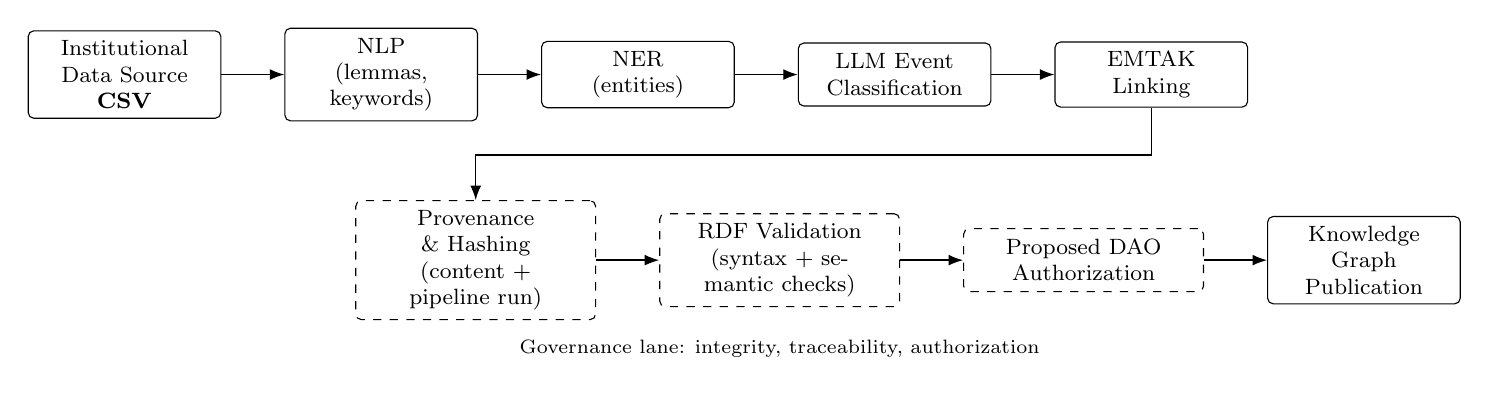
\begin{tikzpicture}[
    font=\footnotesize,
    box/.style={draw, rounded corners=2pt, align=center, inner sep=3.5pt, minimum height=8mm, text width=22mm},
    gbox/.style={draw, dashed, rounded corners=2pt, align=center, inner sep=3.5pt, minimum height=8mm, text width=28mm},
    arrow/.style={-Latex, line width=0.5pt}
]

% --- Top row: processing pipeline ---
\node[box] (csv) {Institutional\\Data Source\\\textbf{CSV}};
\node[box, right=8mm of csv] (nlp) {NLP\\(lemmas,\\keywords)};
\node[box, right=8mm of nlp] (ner) {NER\\(entities)};
\node[box, right=8mm of ner] (llm) {LLM Event\\Classification};
\node[box, right=8mm of llm] (emtak) {EMTAK\\Linking};

\draw[arrow] (csv) -- (nlp);
\draw[arrow] (nlp) -- (ner);
\draw[arrow] (ner) -- (llm);
\draw[arrow] (llm) -- (emtak);

% --- Bottom row: governance lane ---
\node[gbox, below=10mm of nlp, xshift=12mm] (prov) {Provenance \& Hashing\\(content + pipeline run)};
\node[gbox, right=8mm of prov] (val) {RDF Validation\\(syntax + semantic checks)};
\node[gbox, right=8mm of val] (dao) {Proposed DAO\\Authorization};
\node[box, right=8mm of dao, text width=22mm] (pub) {Knowledge Graph\\Publication};

\draw[arrow] (prov) -- (val);
\draw[arrow] (val) -- (dao);
\draw[arrow] (dao) -- (pub);

% --- Fixed clean drop from EMTAK to Provenance (enters prov from the north) ---
\coordinate (emd) at ($(emtak.south)+(0,-6mm)$);
\draw[arrow] (emtak.south) -- (emd) -| (prov.north);

% --- Label under governance lane ---
\node[below=3mm of val, font=\scriptsize] {Governance lane: integrity, traceability, authorization};

\end{tikzpicture}%
}
\caption{Running-case pipeline with the proposed governance intervention: semantic enrichment produces a candidate RDF update; provenance capture and validation establish its technical eligibility, while DAO-mediated authorization determines whether it may become an authoritative graph state.}
\label{fig:runningcase_pipeline}
\end{figure*}

Figure~\ref{fig:runningcase_pipeline} separates two analytically distinct concerns. The upper lane represents the existing semantic-processing problem context: source data are transformed through NLP, NER, LLM classification, and EMTAK linking. In the lower lane, provenance capture and validation are technical preconditions for publication. The proposed DAO authorization step is the design intervention examined in this paper: it should bind an accountable collective decision to the transition from a technically eligible candidate to an authoritative semantic asset. This separation prevents technical validity from being treated as equivalent to institutional authorization.

\paragraph{Institutional Actors and Roles.}
The case assumes a multi-actor institutional environment involving:

\begin{itemize}
    \item \textbf{Content Producers} (e.g., ERR journalists) who generate primary media content;
    \item \textbf{Data Engineers and Curators} who manage ingestion, transformation, and RDF generation;
    \item \textbf{Model Maintainers} responsible for NLP, NER, and LLM configurations and versioning;
    \item \textbf{Validators} who execute syntactic and semantic checks based on the Shapes Constraint Language (SHACL) \cite{Knublauch2017SHACL} and the SPARQL Protocol and RDF Query Language (SPARQL) \cite{Harris2013SPARQL} prior to publication;
    \item \textbf{Institutional Authorities} (e.g., ministries) who rely on the resulting knowledge graph for analytical decision support;
    \item \textbf{Auditors} who may retrospectively inspect provenance chains and authorization decisions.
\end{itemize}

These actors do not operate in isolation. Each modification to the
pipeline, model version, or dataset partition may affect the semantic
interpretation of employment statistics and thereby influence public
reporting or policy evaluation
\cite{Dibowski2024TraceabilityKG,Lebo2013PROVO}. Consequently, governance must extend beyond technical validation and
incorporate explicit authorization and traceability mechanisms
\cite{Schwabe2020KGTrustGovernance,FaqirRhazoui2020DAOOverview}.

\begin{table*}[t]
\caption{Running-case actor model: responsibilities and governance risks across the semantic-asset lifecycle.}
\label{tab:runningcase_actors}
\centering
\renewcommand{\arraystretch}{1.15}
\setlength{\tabcolsep}{3.5pt}
\begin{tabular}{p{5.0cm} p{6cm} p{6cm}}
\hline
\textbf{Actor} & \textbf{Primary responsibility} & \textbf{Governance risk if uncontrolled} \\
\hline
Content producer (publisher) &
Publishes authoritative source text and metadata (e.g., ERR article and date). &
Source authenticity disputes; retroactive edits without traceability; inability to prove who published or changed the source. \\

Data engineer / curator &
Ingests CSV, normalizes records, and triggers RDF generation for the dataset batch. &
Silent dataset mixing (modality/year); inconsistent identifiers; untracked pipeline deviations. \\

NLP/NER model maintainer &
Maintains EstBERT, KeyBERT, and Estonian-language NER configurations and versions used for annotation. &
Model drift and non-reproducible annotations; unannounced version changes; biased or unstable outputs. \\

LLM classification maintainer &
Maintains prompts, parameters, and decision thresholds for employment-event and EMTAK inference. &
Hallucinated or weakly supported claims; threshold gaming; opaque prompt changes affecting results. \\

Validator (technical) &
Runs RDF syntax and semantic checks; executes SPARQL/shape constraints prior to acceptance. &
Acceptance of malformed graphs; missing links in the provenance chain; inconsistent graph structures across versions. \\

Institutional approver (governance authority) &
Authorizes publication/updates of validated semantic assets; decides on corrections and reprocessing. &
Unaccountable approval decisions; delayed corrections; inconsistent policy enforcement across assets. \\

Auditor (internal/external) &
Reviews provenance trails, approvals, and version history for compliance and accountability. &
Non-auditable lifecycle; inability to attribute responsibility; weakened legal and reputational defensibility. \\
\hline
\end{tabular}
\end{table*}

Table~\ref{tab:runningcase_actors} makes the running-case governance problem explicit by mapping institutional roles to their responsibilities and the corresponding failure modes if lifecycle control is absent. The table highlights that technical provenance alone is insufficient: the semantic-asset lifecycle spans multiple human and software actors, including model maintainers and institutional approvers, whose actions can change graph meaning without necessarily violating RDF syntax. This actor–risk decomposition motivates the need for an integrated governance mechanism in which (i) pipeline executions are provenance-bound and reproducible, (ii) validation is enforced prior to state transitions, and (iii) publication and updates are subject to explicit, accountable authorization \cite{Moreau2013PROV,Lebo2013PROVO,Hassan2021DAO}.


\paragraph{Semantic Assets and Graph Structure.}
The assets managed in this case are not monolithic graphs but modular RDF
partitions: separately identifiable graph segments that can be versioned and
governed. The prefixes \texttt{ex:} and \texttt{emp:} below are illustrative
namespace abbreviations used only to keep the example readable. The
illustrative instance demonstrates how a single article results in a
structured semantic artifact comprising:

\begin{itemize}
    \item An \texttt{ex:Article} instance with textual metadata;
    \item Entity nodes (organizations, persons, locations);
    \item Employment classification triples (\texttt{emp:employmentEvent}, \texttt{emp:jobCount});
    \item EMTAK sector links;
    \item Provenance statements using the World Wide Web Consortium (W3C) PROV Ontology (PROV-O), including \texttt{prov:wasGeneratedBy} and time stamps \cite{Lebo2013PROVO};
    \item A processing trajectory that records each computational stage;
    \item Validation queries ensuring structural correctness.
\end{itemize}

The pipeline explicitly records model names, versions, content hashes, and provenance hashes \cite{Moreau2013PROV,Lebo2013PROVO}. A content hash is a compact cryptographic fingerprint: if the graph content changes, its expected hash also changes. These records transform each RDF graph into a verifiable semantic artifact rather than a static representation
\cite{Dibowski2024TraceabilityKG,Carroll2005NamedGraphs}. The knowledge graph thus embodies both domain knowledge and its generation history.

\paragraph{Lifecycle Events.}
The running case reveals that institutional knowledge graphs are subject to recurring lifecycle events:

\begin{itemize}
    \item \textbf{Initial Publication}: New RDF graphs generated from newly ingested articles.
    \item \textbf{Model Update}: Changes in NLP, NER, or LLM versions that may alter semantic outputs.
    \item \textbf{Correction}: Rectification of misclassified employment events or incorrect EMTAK mappings.
    \item \textbf{Reprocessing}: Regeneration of RDF partitions after pipeline improvements.
    \item \textbf{Supersession}: Replacing the active version while retaining its complete history.
    \item \textbf{Deprecation}: Withdrawing a published version from active authoritative use without deleting it.
\end{itemize}

Each of these events affects the semantic state of the graph and may
alter analytical outcomes
\cite{Dibowski2024TraceabilityKG,Moreau2013PROV}. For example, reclassifying an article from neutral reporting to
\texttt{job\_gain} directly influences employment statistics.
Without formal governance, such changes could occur silently,
undermining institutional trust
\cite{Schwabe2020KGTrustGovernance,Hassan2021DAO}.

\paragraph{Governance Requirements Elicited from the Case.}
The running case exposes several governance needs that motivate, but do not yet prescribe, the artifact developed later in the paper.

First, \emph{multi-stakeholder authorization}: decisions about accepting or rejecting RDF outputs involve engineers, data scientists, and institutional authorities \cite{Sandhu1996RBAC,Hassan2021DAO}.

Second, \emph{cross-organizational trust}: EMTAK classifications rely on registry alignment, and employment interpretations rely on LLM outputs with probabilistic confidence values \cite{Schwabe2020KGTrustGovernance,Dibowski2024TraceabilityKG}.

Third, \emph{provenance integrity}: every published semantic asset, and each material claim where claim-level provenance is required, must be traceable to a specific pipeline run, model version, and content hash \cite{Moreau2013PROV,Lebo2013PROVO}.

Fourth, \emph{reproducibility}: trajectory metadata records each transformation step and its configuration, supporting repeatable inspection and qualified re-execution; identical outputs additionally require the relevant models, parameters, dependencies, and sources to be preserved and deterministic \cite{Moreau2013PROV,Dibowski2024TraceabilityKG}.

Fifth, \emph{validation prior to publication}: SPARQL-based tests and structural validation must succeed before the artifact is considered authoritative
\cite{Knublauch2017SHACL,Carroll2005NamedGraphs}.

Collectively, these requirements reveal that governance cannot be reduced to access control lists or editorial approval alone \cite{Schwabe2020KGTrustGovernance,Hassan2021DAO}. Instead, it requires a structured mechanism that binds validation outcomes, provenance records, and authorization decisions into a coherent lifecycle framework \cite{Moreau2013PROV,FaqirRhazoui2020DAOOverview}.

\paragraph{Analytical Scope and Transferability.}
The running case functions as a problem-instantiating scenario, not as an evaluation benchmark or evidence of general effectiveness. It makes visible a set of concerns---verifiable lineage, controlled update authority, multi-actor accountability, and transparent state transitions---that may also arise in regulated private-sector and cross-organizational knowledge graph settings \cite{Hogan2021KnowledgeGraphs,Schwabe2020KGTrustGovernance,Hassan2021DAO}. Whether the resulting design transfers to healthcare, finance, supply chains, or other domains depends on their legal, organizational, and technical constraints and therefore remains a question for subsequent evaluation. In this paper, the case-derived concerns provide requirements against which the DAO-modeling constructs are specialized in Sections~\ref{sec:governance_requirements}--\ref{sec:safeguards}.

\paragraph{Case Selection and Evidential Role.}
The employment-event pipeline was selected purposively because one bounded lifecycle combines the conditions that the artifact must represent: heterogeneous semantic assets, human and software actors, probabilistic extraction, technical validation, cross-organizational reliance, and changes to authoritative status. The unit of analysis is not the hypothetical WoodHive claim itself but the governance of a versioned RDF output from candidate generation through publication, correction, supersession, deprecation, restoration, and archival. The materials available to this study are the pipeline stages, artifact types, actor responsibilities, and failure modes documented in this section and the cited literature; no interviews, observations, or deployed-DAO outcomes are used. A requirement is therefore treated as case-grounded only when it can be traced to a stated actor responsibility or risk in Table~\ref{tab:runningcase_actors}, a listed lifecycle event, or an identified asset/evidence relation. The case supports problem formulation and design demonstration, not claims about how frequently these risks occur, how stakeholders would evaluate the artifact, or whether the design transfers unchanged to another institution.


\subsection{Background Literature}
\label{sec:background}

%\textit{This subsection reviews the scholarly literature relevant to decentralized governance of semantic data infrastructures. It covers prior work on knowledge graph governance and publishing workflows, including centralized authorization models, editorial processes, and provenance-aware publication practices. In addition, it surveys research on blockchain-based governance, with particular attention to decentralized autonomous organizations, smart-contract–based authorization, and collective decision-making mechanisms.}

%\textit{The discussion highlights how existing work in these areas addresses governance and authorization in isolation, but rarely integrates decentralized decision-making directly with the lifecycle of semantic data assets. Rather than providing an exhaustive survey, the subsection synthesizes key concepts, assumptions, and limitations that are directly relevant to the research questions posed in this paper. This synthesis establishes the theoretical grounding for the governance requirements and mechanisms introduced in Sections 3–5.}

The running case combines two objects that are often modeled separately: an evolving semantic asset and the organization that authorizes changes to it. The background therefore proceeds from knowledge graph lifecycle concepts to institutional authorization and then to the model-driven DAO constructs used in the artifact. Its purpose is not to repeat the state-of-the-art gap established in Section~\ref{sec:introduction}, but to define the concepts and relationships on which the subsequent design reasoning depends.

\paragraph{Semantic Assets and Lifecycle Transitions.}
Knowledge graph engineering provides the means to represent, integrate, validate, query, and publish interconnected data \cite{Hogan2021KnowledgeGraphs,Fensel2020KG}. For this study, the relevant unit of governance is a \emph{semantic asset}: a versioned RDF dataset, named graph, ontology, shape set, mapping, or associated processing configuration whose status may change over time. A named graph is an identified group of RDF statements. An ontology or vocabulary defines the concepts and relationships used by the graph; a shape set states constraints used to validate it; and a mapping specifies how source data become graph statements. Lifecycle approaches recognize that these assets undergo recurrent integration, update, validation, and publication activities \cite{Carroll2005NamedGraphs,Cyganiak2014RDFConcepts,Geisler2025KGLifecycle}. A \emph{lifecycle transition} is a governed change in an asset's institutional status---for example, from candidate to validated, published, superseded, deprecated, or archived. Authorization is modeled separately as the governance status of a decision that permits, but does not itself complete, an asset-state transition. Sections~\ref{sec:governance_requirements} and~\ref{sec:dao_mechanisms} use these concepts to specify what is governed and which decisions can change authoritative graph state.

\paragraph{Provenance, Validation, and Authoritativeness.}
Provenance and validation answer different questions. The W3C PROV family represents entities, activities, agents, attribution, and derivation, thereby supporting lineage and retrospective audit \cite{Moreau2013PROV,Lebo2013PROVO}. SHACL or comparable constraints can test whether an RDF candidate satisfies specified structural and semantic conditions \cite{Knublauch2017SHACL}. Cryptographic hashes can bind a governance record to a particular off-chain graph representation or processing result. In the WoodHive example, provenance identifies the article and processing run, validation checks the resulting employment graph, and a hash identifies the exact graph content. None of these mechanisms alone makes the candidate authoritative: authorization is the separate institutional decision to accept the transition. This distinction underpins the separation of evidence, eligibility, and decision rights in Sections~\ref{sec:governance_requirements}--\ref{sec:safeguards}.

\paragraph{Institutional Authority and Collective Authorization.}
Institutional governance allocates responsibility and decision rights among differentiated actors. Role-based access control provides a basis for assigning permissions, but permission to perform an operation does not by itself specify how several actors deliberate, reach a valid collective decision, or remain accountable for its consequences \cite{Sandhu1996RBAC}. DAOs add programmable proposal, voting, quorum, temporal, delegation, and execution mechanisms through which collective decisions can be recorded and, where appropriate, enacted by smart contracts \cite{FaqirRhazoui2020DAOOverview,Hassan2021DAO,Han2025DAOReview}. Their distribution across deliberative forums, off-chain voting, and on-chain execution nevertheless creates a binding problem: a recorded vote does not automatically establish that the correct off-chain graph was validated, published, or reversed \cite{Weidener2026Metagovernance}. In this paper, decentralized authorization therefore denotes a traceable collective decision governed by explicit roles and decision rules; it does not imply that every lifecycle operation occurs on-chain. Nor is a digitally recorded committee decision sufficient by itself to qualify as decentralized. For a critical transition, authority must be distributed across at least two independently accountable principals, no single actor may control proposal, validation, authorization, and confirmation end to end, and any exceptional concentration of authority must be explicitly bounded, visible, and reviewable. The precise number and institutional composition of those principals remain deployment-specific, but the distribution constraint and the evidence used to assess it are part of the artifact specification.

\paragraph{DAO-ML, ET-DM, and DAOMod.}
The artifact uses a model-driven account of DAO governance rather than treating a DAO as an undifferentiated voting contract. DAO-ML supplies the \emph{Organization layer}: constructs for DAOs, roles, committees, governance areas, permissions, and organizational relations \cite{Avanzo2024DAOML}. These constructs provide the basis for representing who may propose, validate, approve, audit, or otherwise participate in a semantic-asset transition. ET-DM supplies complementary \emph{Coordination} and \emph{Execution} layers: decision-making protocols and token-economy elements describe how collective choices are formed, while smart-contract and on-chain/off-chain function constructs describe how accepted choices are operationalized \cite{Avanzo2025ETDM}. DAOMod integrates these layers into an ontology, graphical language, and stepwise method for platform-independent DAO design \cite{Avanzo2025DAOMod}. Model-to-code and subsequent coordination work further illustrate how specified governance constructs can be connected to Solidity implementation and detailed token-economy and voting-protocol models \cite{Avanzo2025DAOMLtoSolidity,Avanzo2026DAOModCoordination}.

These models are foundations rather than completed solutions for the present domain. Section~\ref{sec:governance_requirements} specializes DAO-ML organizational constructs for semantic assets, lifecycle roles, permissions, and decision rights. Section~\ref{sec:dao_mechanisms} specializes ET-DM coordination and execution constructs for proposals over graph-state transitions and for their on-chain/off-chain enactment. Section~\ref{sec:safeguards} adds institutional constraints that are not obtained merely by instantiating generic DAO constructs, including provenance binding, accountable override and reversal, compliance, and resistance to governance capture.

\paragraph{Conceptual Synthesis and Design Boundary.}
The resulting design vocabulary distinguishes four linked but non-equivalent elements: a semantic asset and its lifecycle state; evidence concerning provenance, integrity, and validation; an organizational allocation of roles and permissions; and a coordination-and-execution mechanism that authorizes and enacts a transition. A trustworthy transition requires explicit relations among all four. At the same time, an on-chain authorization record cannot by itself prove legal compliance, semantic correctness, or faithful completion of an off-chain publication action. This boundary guides both the safeguards in Section~\ref{sec:safeguards} and the interpretation of the contract-level evaluation in Section~\ref{sec:evaluation}.

Four record types connect a decision to its consequence and are kept distinct
throughout the paper. An \emph{acceptance decision} is the terminal collective
outcome permitting a stated transition; it is not evidence that execution
occurred. An \emph{authorization record} turns that outcome into a scoped and
possibly expiring permit. A \emph{binding} connects the permit to one exact
operation, input version, and executor. An \emph{execution receipt} is the
executor's attributable report of the observed result, including failure where
applicable. The ordered collection of these records and their provenance forms
the audit path used later.

\paragraph{End-to-End Logical Chain.}
The relations among these concepts are sequential but not substitutable. A
\emph{processing trajectory} records how a candidate graph was produced,
including its stages, inputs, configurations, and outputs; provenance links
that trajectory and the resulting graph to their sources, activities, agents,
and models. Validation then tests whether the identified candidate satisfies
the declared technical and semantic constraints, establishing eligibility for
consideration rather than institutional authority. An acceptance decision
grants or withholds collective approval for the specified transition. If
accepted, an authorization record and binding constrain the approved action to
the exact graph version, operation, and executor. A smart contract can record
and enforce that authorization, but it does not itself perform an off-chain RDF
publication. The publication adapter performs the operation and returns an
attributable execution receipt, which records the observed result without
retroactively proving that the decision was legitimate. In the WoodHive case,
this chain connects extraction of the employment claim to its evidence,
validation, committee decision, scoped publication authority, and confirmed
graph-state change. Each link answers a different assurance question, so
omitting one cannot be compensated for by strengthening another.

Accordingly, the design proceeds through a traceable specialization. Constructs taken unchanged from DAO-ML, ET-DM, and DAOMod are treated as inherited foundations; constructs assigned knowledge-graph meanings are treated as domain adaptations; and safeguards required by the institutional setting are identified as new extensions. The running-case requirements and this layered knowledge base jointly provide the premises for the artifact construction beginning in Section~\ref{sec:governance_requirements}.

\subsection{Requirement Derivation and Traceability Protocol}
\label{sec:derivation_protocol}

Following the design-science distinction between the problem environment, the knowledge base, and the constructed artifact \cite{hevner2004design}, the requirements were derived through a documented five-stage procedure. First, the case description was decomposed into an inventory of governed asset types, lifecycle events, actors, responsibilities, evidence objects, and failure modes. Second, each concern was normalized as a requirement by identifying the governed object, responsible or eligible actor, operation or decision, precondition or constraint, and evidence needed to verify compliance. Third, each normalized requirement was matched to the relevant DAOMod layer: DAO-ML Organization for assets, roles, scopes, and permissions; ET-DM Coordination for proposal and collective-decision rules; ET-DM Execution for authorization binding and observable enactment; or an institutional safeguard when generic constructs did not adequately represent the concern. Fourth, each construct was classified as inherited, adapted, or extended. Finally, forward and backward traceability were checked: every case concern had to map to at least one requirement and design construct, and every requirement had to map back to a stated case concern, an upstream requirement, or a cited knowledge-base premise.

The procedure was applied sequentially across Sections~\ref{sec:governance_requirements}--\ref{sec:safeguards}. The Organization-layer requirements (OLR1--OLR12) are inputs to the Coordination and Execution requirements (CR1--CR6 and ER1--ER6), which in turn expose the risks addressed by the safeguard requirements (SG1--SG12). Within each stage, candidate statements with the same governed object, control, and evidence obligation were merged; a candidate was excluded if it merely repeated an implementation choice, could not be traced to the case or knowledge base, or belonged to a later layer. The consolidated tables report the resulting identifier, requirement, model treatment, and rationale, allowing another analyst to repeat the mapping and challenge individual derivation steps.

Completeness is assessed relative to this analytical frame rather than claimed universally. The derivation is internally complete when every actor, responsibility, and failure mode in Table~\ref{tab:runningcase_actors} is covered; every lifecycle event in Section~\ref{sec:runningcase} has an identifiable authority, decision path, execution consequence, and evidence trail; successful, rejected, failed, stale, challenged, and exceptional paths terminate in an explicit state; and every requirement is traceable in both directions. The authors conducted the analytical walkthrough summarized in Table~\ref{tab:derivation_coverage} as part of artifact construction and found no uncovered element within this bounded frame. No independent requirements panel or inter-rater reliability assessment was used. The result is therefore design completeness for the stated case and model boundary, not empirical saturation, stakeholder acceptance, legal sufficiency, or completeness for other domains.

\begin{table*}[t]
\caption{Coverage dimensions used for the analytical-completeness walkthrough}
\label{tab:derivation_coverage}
\centering
\renewcommand{\arraystretch}{1.10}
\setlength{\tabcolsep}{4pt}
\begin{tabular}{p{3.0cm}p{6.2cm}p{7.4cm}}
\hline
\textbf{Input dimension} & \textbf{Closure question} & \textbf{Requirement families providing coverage}\\
\hline
Assets and lifecycle & Is every governed asset/version and listed transition identifiable, state-bounded, and evidence-linked? & OLR1--OLR3, OLR9; CR1, CR4; ER3--ER6; SG2, SG4, SG7--SG9\\
Actors and authority & Does every stated responsibility or risk have scoped authority, incompatibility, delegation, and accountability controls? & OLR4--OLR8, OLR10--OLR12; CR2, CR6; ER1; SG1, SG5--SG6, SG10--SG11\\
Collective decision & Can admission, participation, policy, outcome, challenge, and governance change be represented without conflation? & OLR5--OLR6, OLR11--OLR12; CR1--CR6; SG3, SG9--SG12\\
Execution and evidence & Can an accepted decision be traced to one exact operation, receipt, result, and failure state? & ER1--ER6; SG2, SG4, SG8, SG12\\
Exceptional and recovery paths & Are correction, restoration, emergency action, appeal, deadlock, timeout, and non-execution explicit and reviewable? & OLR8, OLR10, OLR12; CR5--CR6; ER2, ER5--ER6; SG4--SG12\\
\hline
\end{tabular}
\end{table*}


\section{DAO-ML Organization-Layer Specialization for Institutional Knowledge Graph Lifecycles}
\label{sec:governance_requirements}

Section~\ref{sec:runningcase} established that an institutional knowledge graph is governed through decisions about identifiable semantic assets, responsible roles, and changes in authoritative status. Section~\ref{sec:background} established that DAO-ML provides reusable Organization-layer constructs---including DAOs, roles, committees, governance areas, permissions, and organizational relations---but does not assign them knowledge-graph lifecycle semantics \cite{Avanzo2024DAOML,Avanzo2025DAOMod}. This section develops the organizational specialization required by RQ1. It remains at the platform-independent modeling level: proposal processes, voting rules, and on-chain/off-chain execution are deferred to the ET-DM specialization in Section~\ref{sec:dao_mechanisms}, while institutional safeguards are developed in Section~\ref{sec:safeguards}.

Throughout Sections~\ref{sec:governance_requirements}--\ref{sec:safeguards},
normative verbs such as ``must,'' ``requires,'' and ``prevents'' specify
properties of the platform-independent design; they are not reports that the
pilot implements or empirically verifies those properties. Section~\ref{sec:evaluation}
tests this distinction requirement by requirement: an E status denotes direct
exercised support for every contract-observable clause, P denotes partial
representation or execution, and N denotes no reachable implementation. Thus,
the design propositions in these sections are supported by requirements
derivation and formal specification, whereas only the subset identified by
the E/P/N crosswalk receives implementation evidence.

The requirements are derived by matching the running-case elements to the DAO-ML Organization layer under the protocol in Section~\ref{sec:derivation_protocol}. For each case element, the analysis asks whether an existing DAO-ML construct can be inherited unchanged, requires a domain-specific interpretation, or must be complemented by a knowledge-graph-specific extension. Figure~\ref{fig:org_specialization_taxonomy} summarizes the resulting four-part structure: governed semantic assets and lifecycle scope; specialized organizational roles and bodies; transition-scoped permissions and decision rights; and explicit organizational constraints and evidence associations. The section ends with the design-stage answer to RQ1 and a consolidated specification against which the implementation can later be evaluated.

\begin{figure}[t]
\centering
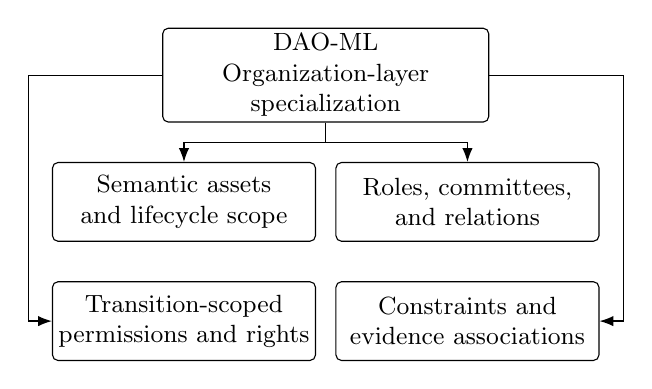
\begin{tikzpicture}[
    font=\small,
    root/.style={draw, rounded corners=2pt, align=center, text width=40mm, minimum height=8mm, inner sep=2pt},
    child/.style={draw, rounded corners=2pt, align=center, text width=32mm, minimum height=10mm, inner sep=2pt},
    arrow/.style={-Latex, line width=0.45pt}
]
\node[root] (root) {DAO-ML Organization-layer\\specialization};
\node[child, below=5mm of root, xshift=-18mm] (assets) {Semantic assets\\and lifecycle scope};
\node[child, below=5mm of root, xshift=18mm] (roles) {Roles, committees,\\and relations};
\node[child, below=5mm of assets] (rights) {Transition-scoped\\permissions and rights};
\node[child, below=5mm of roles] (constraints) {Constraints and\\evidence associations};
\draw[arrow] (root.south) -- ++(0,-2.5mm) -| (assets.north);
\draw[arrow] (root.south) -- ++(0,-2.5mm) -| (roles.north);
\draw[arrow] (root.west) -- ++(-17mm,0) |- (rights.west);
\draw[arrow] (root.east) -- ++(17mm,0) |- (constraints.east);
\end{tikzpicture}
\caption{Organization-layer specialization required to represent institutional knowledge graph governance.}
\label{fig:org_specialization_taxonomy}
\end{figure}

\subsection{Semantic Assets and Lifecycle Scope}
\label{sec:lifecycle}

DAO-ML governance areas identify subjects over which organizational authority is exercised \cite{Avanzo2024DAOML}. For institutional knowledge graph governance, that scope must be made more precise by introducing the domain concept \emph{SemanticAsset}. A semantic asset is a separately identifiable and versioned RDF dataset, named graph, ontology, vocabulary, shape set, mapping, or processing configuration whose institutional status can be governed. In the running case, examples include an employment-event graph partition, an EMTAK mapping, a validation shape set, and a versioned extraction configuration. Provenance records and validation reports are treated as evidence associated with an asset version rather than automatically as independently governed assets; an institution may nevertheless promote them to assets when their own lifecycle requires governance.

Each semantic asset requires a stable identifier, an asset type, a version identifier, and a reference to its off-chain representation. This extension is necessary because a general governance area can state the organizational domain of authority but cannot, without domain specialization, identify the exact graph version affected by a permission or decision. The specialization therefore relates each DAO-ML governance area to one or more semantic assets and lifecycle-transition types.

Let $A$ be the set of semantic assets, $V_a$ the versions of asset $a\in A$, $V=\bigcup_{a\in A}V_a$, $owner:V\rightarrow A$ the version-to-asset function, and $O$ the permitted lifecycle operations. Equation~\ref{eq:lifecycle_states} defines the lifecycle-state vocabulary:
\begin{equation}
\label{eq:lifecycle_states}
\begin{aligned}
S=\{&\mathit{candidate},\mathit{validated},\mathit{published},\\
&\mathit{superseded},\mathit{deprecated},\mathit{archived}\}.
\end{aligned}
\end{equation}
A \emph{tuple} is an ordered collection in
which each position has a defined meaning. An atomic version transition is
$\tau=(v,s_i,o,s_j)\in V\times S\times O\times S$. In ordinary language, this
tuple states that operation $o$ moves version $v$ from source state $s_i$ to
target state $s_j$.

A governed transition plan is a non-empty finite set $g=\{\tau_1,\ldots,\tau_n\}$. It is well formed for asset $a$, written $PlanFor(g,a)$, only if every affected version belongs to $a$, no version is assigned conflicting source or target states, and the operations jointly satisfy the lifecycle invariants, including that at most one version is current after confirmation. All members of a well-formed plan must either be confirmed together or remain unconfirmed. Let $T$ be the set of named plan types and $type(g)\in T$ the type of plan $g$; an elementary plan has $|g|=1$. Replacement and restoration are compound because they change which of two retained versions is authoritative.

For example, suppose the published WoodHive employment graph is $v_{old}$ and reprocessing produces a validated correction $v_{new}$. Replacement couples $(v_{new},\mathit{validated},\mathit{publish},\mathit{published})$ with $(v_{old},\mathit{published},\mathit{supersede},\mathit{superseded})$. Both changes must succeed together; otherwise the institution could expose two current versions or none. A correction therefore creates a new candidate rather than modifying the published version in place. Restoration uses the same forward-only pattern for a retained superseded, deprecated, or archived version, so it never erases the intervening history \cite{Moreau2013PROV,Lebo2013PROVO,Dibowski2024TraceabilityKG}. Authorization remains a separate governance status attached to the decision and execution binding; it is not itself a lifecycle state.

\begin{table}[t]
\caption{Lifecycle scope represented by the Organization-layer specialization}
\label{tab:lifecycle_requirements}
\centering
\begin{tabular}{p{1.9cm}p{2.3cm}p{3.1cm}}
\hline
Operation & State change & Organizational significance\\
\hline
Validate & Candidate $\rightarrow$ Validated & Records technical eligibility; does not confer authority\\
Publish & Validated $\rightarrow$ Published & Requires an accepted decision and scoped authorization record\\
Replace & New validated $\rightarrow$ published; old published $\rightarrow$ superseded & Atomically changes which retained version is authoritative\\
Deprecate & Published $\rightarrow$ Deprecated & Withdraws an asset from active authoritative use\\
Restore & Prior superseded/deprecated/archived $\rightarrow$ published; current published $\rightarrow$ superseded & Re-authorizes a prior version without deleting history\\
Archive & Superseded/deprecated $\rightarrow$ Archived & Retains history outside active use\\
\hline
\end{tabular}
\end{table}

Table~\ref{tab:lifecycle_requirements} translates the formal state vocabulary
into the six lifecycle operations used by the design and explains why each
transition matters organizationally. It is not a repetition of
Eq.~\ref{eq:lifecycle_states}: the equation defines the allowed states, whereas
the table associates state changes with governance consequences. This state
vocabulary is a domain extension rather than a claim that DAO-ML itself
defines a knowledge graph lifecycle. Its organizational purpose is to provide
the scope needed to express which role or committee holds which permission
over which asset and transition. The conditions and sequencing by which a
proposal produces one of these transitions belong to the Coordination and
Execution layers developed in Section~\ref{sec:dao_mechanisms}.

\subsection{Specialized Roles, Committees, and Organizational Relations}
\label{sec:roles}

DAO-ML roles, committees, and organizational relations can be inherited, but their responsibilities must be specialized for the running case \cite{Avanzo2024DAOML}. Roles remain functional assignments rather than job titles: one person may hold several roles, and a role may be occupied by actors from different institutions. Such assignments do not remove the need to express separation-of-duty constraints where a critical transition must not be controlled by one actor.

The running case yields seven role specializations. A \emph{Producer} supplies source content or initiates a candidate asset. A \emph{Curator} prepares, corrects, and versions semantic assets. A \emph{ModelMaintainer} is responsible for the models, prompts, thresholds, or vocabularies used to generate candidate claims. A \emph{Validator} records validation evidence but does not thereby authorize publication. An \emph{Authorizer} participates in the institutional decision over a lifecycle transition. An \emph{Auditor} inspects assets, evidence, role assignments, and decision histories and may initiate a challenge; veto or revocation authority is not implied merely by being an auditor. Finally, an \emph{EmergencyAuthority} is an optional exceptional role or committee whose powers must be expressly assigned and constrained.

Collective authority is represented through a DAO-ML committee rather than by granting identical individual permissions to an unspecified group. For example, a PublicationCommittee may include authorizers from participating institutions, whereas a ValidationCommittee may aggregate domain and technical validators. Committee membership and relations to governance areas make institutional responsibility visible at the organizational layer; quorum, voting weight, decision rules, and temporal windows remain ET-DM coordination concerns.

\begin{table}[t]
\caption{Running-case specialization of DAO-ML organizational constructs}
\label{tab:governance_roles}
\centering
\begin{tabular}{p{2.1cm}p{1.8cm}p{3.4cm}}
\hline
Specialization & DAO-ML basis & Organizational responsibility\\
\hline
Producer & Role & Submit a sourced candidate asset\\
Curator & Role & Prepare and version semantic content\\
ModelMaintainer & Role & Maintain generation configurations and versions\\
Validator & Role/Committee & Produce technical or expert validation evidence\\
Authorizer & Role/Committee & Exercise assigned transition authority\\
Auditor & Role & Inspect records and initiate challenges\\
EmergencyAuthority & Role/Committee & Exercise expressly bounded exceptional powers\\
Semantic domain & GovernanceArea & Scope authority to asset classes and transitions\\
\hline
\end{tabular}
\end{table}

Table~\ref{tab:governance_roles} provides the crosswalk from each running-case
specialization to its DAO-ML basis and responsibility. Its contribution is to
show which concepts are inherited roles or committees and which semantic
domain scope must be added; it is therefore used to derive the permission
assignments that follow. Organizational relations must additionally represent
role membership, committee membership, responsibility for a governance area,
delegation between eligible roles, and incompatibility between assignments.
These relations permit the model to distinguish collaboration from authority
and evidence production from authorization. They also preserve a central
distinction established in Section~\ref{sec:background}: semantic validity is
evidence considered by governance, not a substitute for governance.

\subsection{Transition-Scoped Permissions and Decision Rights}
\label{sec:decision_rights}

Generic read and write privileges are insufficient for authoritative knowledge graph evolution. DAO-ML permissions must be specialized by both semantic-asset scope and lifecycle-transition type. Equation~\ref{eq:permission_vocabulary} defines the relevant permission vocabulary:
\begin{equation}
\label{eq:permission_vocabulary}
\begin{aligned}
P=\{&\mathit{propose},\mathit{prepare},\mathit{validate},\mathit{authorize},\\
&\mathit{execute},\mathit{challenge},\mathit{delegate},\mathit{administer}\}.
\end{aligned}
\end{equation}
The distinction among \emph{validate}, \emph{authorize}, and \emph{execute} is essential. Validation attests that stated technical or semantic conditions have been checked. Authorization records an institutionally valid decision. Execution performs or requests the corresponding on-chain or off-chain operation. Assigning one permission never implies the other two.

Let $R$ and $C$ denote roles and committees. Equation~\ref{eq:decision_rights} represents decision-right assignments:
\begin{equation}
\label{eq:decision_rights}
\delta:(R\cup C)\times A\times T\rightarrow 2^P.
\end{equation}
Thus, the same role may propose a correction to one asset class while lacking authority to approve its publication, and a committee may authorize deprecation without being permitted to execute the off-chain deletion or archival operation. Organizational eligibility for an action can be expressed as
\begin{equation}
\label{eq:organizational_eligibility}
Eligible(x,a,t,p)\iff p\in\delta(x,a,t),
\end{equation}
where $x\in R\cup C$, $a\in A$, $t\in T$, and $p\in P$. Equation~\ref{eq:organizational_eligibility} establishes who is organizationally eligible; it does not assert that a proposal has met quorum, timing, evidence, or execution conditions. Those conditions are added by the later ET-DM and safeguard specializations.

The expression can be read as a four-part permission check: actor construct $x$ may exercise permission $p$ only for asset $a$ and transition type $t$. Thus, a WoodHive curator may be eligible to propose reprocessing but still be ineligible to authorize publication of the resulting version.

\begin{table}[t]
\caption{Illustrative transition-scoped decision-right assignments}
\label{tab:decision_rights}
\centering
\begin{tabular}{p{2.0cm}p{2.1cm}p{3.2cm}}
\hline
Transition & Eligible construct & Permission\\
\hline
Create candidate & Producer/Curator & Propose, prepare\\
Record validation & Validator or ValidationCommittee & Validate\\
Authorize publication & Authorizer or PublicationCommittee & Authorize\\
Execute publication & Assigned executor & Execute\\
Propose reprocessing & ModelMaintainer/Curator & Propose\\
Challenge a decision & Auditor & Challenge\\
Exceptional restoration & EmergencyAuthority & Propose or authorize only as expressly assigned\\
Change an assignment & Governance administrator or committee & Administer\\
\hline
\end{tabular}
\end{table}

Table~\ref{tab:decision_rights} demonstrates how
Eq.~\ref{eq:decision_rights} separates proposing, validating, authorizing,
executing, challenging, and administering. The assignments are illustrative,
not a universal staffing prescription; their analytical contribution is to
make permission separation concrete before delegation and incompatibility
constraints are introduced. Delegation must also be represented as a scoped
relation rather than as an unrestricted transfer of role identity. A
delegation identifies the delegating and receiving roles, affected governance
area, permitted transition types, and validity interval. Whether such a
delegation is approved, activated, or revoked is a coordination question; the
Organization layer must nevertheless contain enough information to prevent a
delegated permission from silently expanding beyond its original asset and
transition scope.

\subsection{Consolidated Organization-Layer Requirements}
\label{sec:constraints}

The KG specialization can be summarized by Eq.~\ref{eq:organization_specialization}:
\begin{equation}
\label{eq:organization_specialization}
\begin{aligned}
\mathcal{O}_{KG}=\langle&D,U,\Pi,R,C,G,A,S,T,P,E,\\
&\rho,\sigma,\delta,\epsilon,\chi\rangle,
\end{aligned}
\end{equation}
This tuple is a compact inventory of the organizational model, not an execution algorithm. $D$ denotes the DAO; $U$ the participating actors; $\Pi$ the accountable principals such as institutions or independently mandated persons; $R$ and $C$ the roles and committees; $G$ the governance areas; $A$, $S$, and $T$ the assets, lifecycle states, and transition types; $P$ the permissions; and $E$ the evidence categories.

The relations connect those sets. Relation $\rho:U\rightarrow 2^{R\cup C}$ assigns actors to roles and committees, while $principal:U\rightarrow\Pi$ resolves technical actors to accountable principals. Relation $\sigma:G\rightarrow 2^{A\times T}$ scopes governance areas to assets and transitions. Relation $\delta$ assigns transition-scoped permissions, $\epsilon:T\rightarrow 2^E$ states which evidence categories a transition requires, and $\chi:T\rightarrow\mathcal{C}_{dist}$ supplies its distribution constraint from the set $\mathcal{C}_{dist}$ of permitted constraint specifications. For the WoodHive graph, these relations identify the responsible curator and publication committee, the permitted publication transition, and its required provenance, content hash, model version, and validation report. The procedures that assess this information are specified later.

The Organization layer must also expose, for each transition type, a reference to the coordination policy that governs decision formation. Such a reference identifies whether review, a voting window, quorum, an execution delay, or escalation is applicable, without specifying the protocol or numerical values at this layer. This handoff prevents organizational eligibility from being mistaken for a completed authorization decision and provides the input needed by the ET-DM Coordination layer.

For critical transitions, the Organization layer additionally records a distribution constraint $\chi(t)$. Equation~\ref{eq:distributed_transition} states the minimum condition:
\begin{equation}
\label{eq:distributed_transition}
\begin{aligned}
Distributed(t)\iff{}& |IndependentPrincipals(t)|\geq 2\\
&{}\land \neg\exists u\in U\;EndToEndControl(u,t).
\end{aligned}
\end{equation}
$IndependentPrincipals(t)\subseteq\Pi$ is derived from current role and committee assignments and their valid mandates; $EndToEndControl(u,t)$ means that actor $u$ controls proposal, validation, authorization, execution, and confirmation for transition type $t$. Independence is therefore established through accountable mandates rather than by counting technical addresses. A stricter deployment may require representation from several institutions or a larger decision body; an exceptional policy may temporarily relax the ordinary composition only under the bounded and reviewable safeguards defined in Section~\ref{sec:safeguards}. This criterion distinguishes decentralized institutional authorization from a conventional single-actor approval recorded on a ledger.

In ordinary language, the predicate requires at least two independently accountable participants and prohibits any one actor from controlling proposal, validation, authorization, and confirmation. Multiple blockchain addresses controlled by the same institution therefore do not satisfy the condition.

Table~\ref{tab:org_requirements} consolidates the organization-layer requirements (OLRs) derived above. The classification column makes the design provenance explicit: \emph{inherited} constructs retain their DAO-ML meaning, \emph{adapted} constructs receive institutional knowledge graph semantics, and \emph{extended} constructs are introduced because the domain information is not represented by the generic Organization layer.

\begin{table*}[t]
\caption{Consolidated requirements for the DAO-ML Organization-layer specialization}
\label{tab:org_requirements}
\centering
\renewcommand{\arraystretch}{1.12}
\setlength{\tabcolsep}{4pt}
\begin{tabular}{p{1.0cm}p{5.1cm}p{4.1cm}p{5.2cm}}
\hline
\textbf{Identifier} & \textbf{Requirement} & \textbf{DAO-ML treatment} & \textbf{Running-case rationale}\\
\hline
OLR1 & Represent each governed semantic asset and immutable version with a stable reference. & Extended: SemanticAsset and version reference & A decision must identify the exact graph, mapping, shape set, or configuration affected.\\
OLR2 & Represent lifecycle states and permitted transition types separately from asset identity. & Extended: LifecycleState and TransitionType & Publication, replacement, deprecation, restoration, and archival have different meanings.\\
OLR3 & Scope organizational authority to asset classes and transition types. & Adapted: GovernanceArea & Authority over employment-event graphs must not imply authority over every institutional asset.\\
OLR4 & Represent functional lifecycle responsibilities independently of local job titles. & Adapted: Role & Producers, curators, model maintainers, validators, authorizers, and auditors contribute differently.\\
OLR5 & Represent multi-actor authority and membership explicitly. & Inherited and adapted: Committee and organizational relations & Collective institutional authorization requires an identifiable responsible body.\\
OLR6 & Distinguish propose, prepare, validate, authorize, execute, challenge, delegate, and administer permissions. & Adapted: Permission & Technical validation, institutional authorization, and publication execution must not be conflated.\\
OLR7 & Assign permissions jointly by role or committee, semantic asset, and transition type. & Extended permission scope $\delta$ & Rights vary with asset criticality and the requested lifecycle change.\\
OLR8 & Express incompatible assignments and bounded delegation. & Adapted organizational relations plus constraints & A creator must not silently become sole authorizer, and delegation must not broaden authority.\\
OLR9 & Associate transition types with required evidence categories without treating evidence as authorization. & Extended evidence association $\epsilon$ & Provenance, validation, hashes, and model versions inform but do not replace a governance decision.\\
OLR10 & Make changes to roles, committees, scopes, and permissions themselves identifiable governance actions. & Adapted organizational administration & Evolution of the governance configuration must remain attributable and subject to authority.\\
OLR11 & Associate each governed transition type with its applicable coordination-policy reference. & Extended Organization-to-Coordination linkage & Eligible roles still require an explicit decision procedure before authority can be exercised.\\
OLR12 & Record and enforce a distribution constraint for critical transitions. & Extended distribution constraint $\chi$ & At least two independently accountable principals participate and no actor controls proposal, validation, authorization, and confirmation end to end.\\
\hline
\end{tabular}
\end{table*}

\subsection{Design-Stage Answer to RQ1}
At the design stage, RQ1 is answered as follows: the DAO-ML Organization layer must be specialized so that governance concerns identifiable, immutable semantic-asset versions and explicit lifecycle-transition types rather than undifferentiated data resources. Its generic roles, committees, governance areas, permissions, and relations must be given lifecycle-specific meanings; authority must be scoped jointly by actor, asset, transition, and permission; validation evidence must remain distinct from authorization; and governance administration, delegation, incompatible assignments, coordination-policy references, and minimum distribution constraints must be represented explicitly. OLR1--OLR12 operationalize this answer for the stated analytical frame. They form the platform-independent organizational input to RQ2, but do not yet select a voting protocol, quorum, review period, contract function, or publication adapter. Whether an implementation covers these requirements is an evaluation question, not part of this design-stage answer.

\section{ET-DM Coordination and Execution Specialization for Knowledge Graph Lifecycles}
\label{sec:dao_mechanisms}

Section~\ref{sec:governance_requirements} produced OLR1--OLR12 as the organizational input to RQ2. Those requirements identify the governed semantic asset and version, the requested lifecycle transition, eligible roles and committees, scoped permissions, evidence categories, the reference to an applicable coordination policy, and the minimum distribution constraint for critical transitions. They do not yet specify how eligible participants form a valid collective decision or how an accepted decision is bound to an on-chain or off-chain operation. This section specializes the ET-DM Coordination and Execution layers for those purposes \cite{Avanzo2025ETDM,Avanzo2025DAOMod,Avanzo2026DAOModCoordination}.

The specialization follows the same design-provenance distinction used in Section~\ref{sec:governance_requirements}. ET-DM decision-making protocols, token-economy elements, smart-contract primitives, and on-chain/off-chain functions are inherited as modeling foundations. They are adapted by assigning them semantic-asset, lifecycle-transition, and institutional-role meanings. Additional binding and receipt constructs are introduced where a generic DAO decision is insufficient to demonstrate that the authorized graph operation was faithfully executed. Figure~\ref{fig:dao_process} shows the resulting handoff across the artifact layers.

\begin{figure*}[t]
\centering
\resizebox{\textwidth}{!}{%
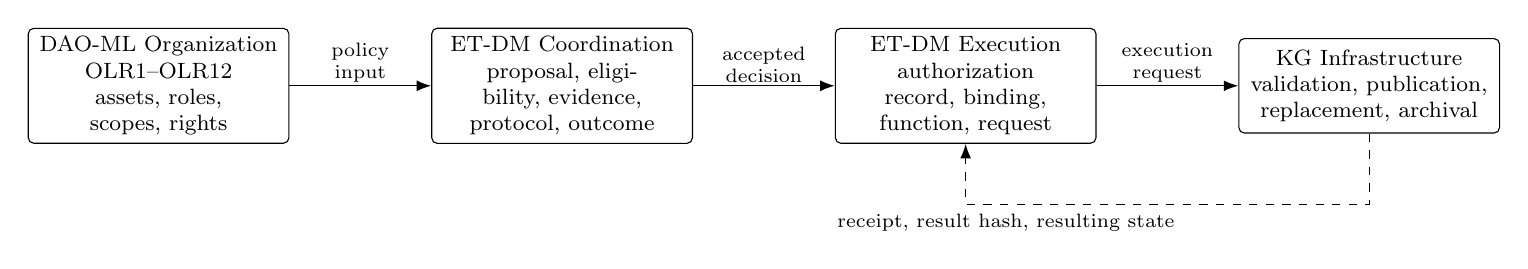
\begin{tikzpicture}[
    font=\footnotesize,
    box/.style={draw, rounded corners=2pt, align=center, text width=31mm, minimum height=12mm, inner sep=3pt},
    arrow/.style={-Latex, line width=0.5pt},
    feedback/.style={-Latex, dashed, line width=0.5pt}
]
\node[box] (org) {DAO-ML Organization\\OLR1--OLR12\\assets, roles, scopes, rights};
\node[box, right=18mm of org] (coord) {ET-DM Coordination\\proposal, eligibility, evidence, protocol, outcome};
\node[box, right=18mm of coord] (exec) {ET-DM Execution\\authorization record, binding, function, request};
\node[box, right=18mm of exec] (kg) {KG Infrastructure\\validation, publication, replacement, archival};
\draw[arrow] (org) -- node[midway,above,align=center,fill=white,inner sep=1pt,font=\scriptsize]{policy\\input} (coord);
\draw[arrow] (coord) -- node[midway,above,align=center,fill=white,inner sep=1pt,font=\scriptsize]{accepted\\decision} (exec);
\draw[arrow] (exec) -- node[midway,above,align=center,fill=white,inner sep=1pt,font=\scriptsize]{execution\\request} (kg);
\draw[feedback] (kg.south) -- ++(0,-9mm) -| node[below,pos=0.45,font=\scriptsize]{receipt, result hash, resulting state} (exec.south);
\end{tikzpicture}%
}
\caption{Layered specialization from DAO-ML organizational eligibility through ET-DM coordination and execution to a technically confirmed knowledge graph lifecycle operation; Section~\ref{sec:safeguards} adds the institutional confirmation gate.}
\label{fig:dao_process}
\end{figure*}

Table~\ref{tab:olr_etdm_mapping} makes the input from Section~\ref{sec:governance_requirements} explicit. The mapping is many-to-many: an organizational requirement may constrain both decision formation and execution, while one ET-DM construct may operationalize several organizational requirements.

\begin{table*}[t]
\caption{Traceability from the organization-layer requirements to the ET-DM specialization}
\label{tab:olr_etdm_mapping}
\centering
\renewcommand{\arraystretch}{1.12}
\setlength{\tabcolsep}{4pt}
\begin{tabular}{p{1.8cm}p{4.1cm}p{3.3cm}p{7.0cm}}
\hline
\textbf{Input} & \textbf{Organizational information} & \textbf{ET-DM layer} & \textbf{Specialization produced in this section}\\
\hline
OLR1--OLR3 & Asset, immutable version, lifecycle transition, governance scope & Coordination and Execution & Proposal and execution binding identify the exact asset version, source state, target state, and operation.\\
OLR4--OLR5 & Functional roles, committees, and memberships & Coordination & Participant eligibility and decision body are derived from current organizational assignments.\\
OLR6--OLR8 & Scoped permissions, incompatible assignments, bounded delegation & Coordination & Protocol admission and vote or approval eligibility are checked against role-, asset-, and transition-scoped rights.\\
OLR9 & Evidence categories & Coordination and Execution & Proposal contains an evidence manifest; execution verifies the referenced asset and evidence hashes.\\
OLR10 & Governable organizational change & Coordination and Execution & Role, committee, scope, and permission changes are represented as proposal and execution types rather than administrative side effects.\\
OLR11 & Coordination-policy reference & Coordination & The transition selects its decision mechanism, eligibility rule, quorum, threshold, timing, and delegation conditions.\\
OLR12 & Distribution constraint & Coordination and safeguards & Admission and acceptance verify independent principals and prohibit unilateral end-to-end control of critical transitions.\\
\hline
\end{tabular}
\end{table*}

\subsection{ET-DM Coordination-Layer Specialization}
\label{sec:dao_decisions}

The Coordination layer transforms organizational eligibility into a decision outcome. Its central artifact is a transition proposal rather than an unrestricted request to edit an RDF store. Each proposal contains an \emph{evidence manifest}: an enumerated list of supporting records, such as provenance, validation results, model versions, and content hashes, together with stable references to them. Equation~\ref{eq:transition_proposal} defines a proposal:
\begin{equation}
\label{eq:transition_proposal}
p=\langle id,a,g,e,i,\kappa\rangle,
\end{equation}
where $id$ is the proposal identifier; $a$ identifies the semantic asset; $g$ is the complete governed transition plan defined in Section~\ref{sec:lifecycle}; $e$ is the evidence manifest; $i\in U$ is the initiating actor, whose organizational role is recovered through $\rho(i)$; and $\kappa$ is the referenced coordination policy. The proposal is admissible only if $PlanFor(g,a)$. The affected versions, their expected source and target states, and the requested operations are recoverable from $g$. In the running case, a proposal to publish the WoodHive employment event fixes the candidate graph version, validation report, source-article provenance, model version, and content hash before collective authorization begins. A replacement or restoration proposal also fixes both coupled version-state changes. Altering any member of $g$ requires a new proposal or an explicitly recorded amendment procedure, because otherwise participants could vote on one operation while another is executed.

The applicable coordination policy is represented by Eq.~\ref{eq:coordination_policy}:
\begin{equation}
\label{eq:coordination_policy}
\begin{aligned}
\kappa_t=\langle& Elig_t,M_t,Q_t,\Theta_t,W_t,Del_t,\\
& I_t,N_t,C_t\rangle,
\end{aligned}
\end{equation}
where $Elig_t$ selects eligible roles or committees from the Organization layer, $M_t$ identifies the decision mechanism, $Q_t$ is the quorum rule, $\Theta_t$ is the acceptance rule, $W_t$ defines review and decision windows, and $Del_t$ defines whether and how participation may be delegated. For critical transitions, $I_t$ declares whether independence is assessed by actor, role, or institution; $N_t>1$ is the required minimum number of independently accountable principals; and $C_t<1$ is the maximum effective decision-authority share of one principal. ET-DM supplies reusable decision-protocol and token-economy concepts; the specialization binds those concepts to lifecycle transitions and organizational mandates \cite{Avanzo2025ETDM,Avanzo2026DAOModCoordination}.

Thus, $\kappa_t$ is a checklist for how transition type $t$ is decided. For publication of the WoodHive graph, it states who may participate, whether the committee votes, how many members must participate, what support is sufficient, how long review remains open, and whether delegation is allowed. The final three elements ensure that formally distinct voters also represent the required independent principals.

Let $a(p)$ denote the asset named by proposal $p$, $g(p)$ its plan, and $t(p)=type(g(p))$. For compactness, let $P_p=CountedParticipants(p)$ and $I_p=I_{t(p)}$. The realized-decision distribution condition is given by Eq.~\ref{eq:decentralized_decision}:
\begin{equation}
\label{eq:decentralized_decision}
\begin{aligned}
&DecentralizedDecision(p,\kappa_{t(p)})\\
&\quad\iff IndependentCount(P_p,I_p)\geq N_{t(p)}\\
&\qquad\land MaxAuthorityShare(P_p,I_p)\leq C_{t(p)}\\
&\qquad\land \neg\exists u\in U\;EndToEndControl(u,t(p)).
\end{aligned}
\end{equation}
$CountedParticipants(p)$ is the set of admitted actors whose participation contributes to proposal $p$; $MaxAuthorityShare$ is the largest share of counted decision weight under the selected policy and, for an unweighted body, is the reciprocal of the applicable independent-principal count. The condition is evaluated against current assignments and valid delegations. It makes decentralization inspectable under the declared policy, but does not by itself establish legitimacy, legal compliance, or resistance to informal influence.

Read plainly, the condition succeeds only when enough independent principals actually participate, none exceeds the permitted share of decision power, and no actor controls the transition from beginning to end. It therefore rules out calling a WoodHive publication decision decentralized merely because one organization uses several accounts.

$Distributed(t)$ is an Organization-layer structural prerequisite: current assignments make distributed control possible. $DecentralizedDecision(p,\kappa_t)$ is a Coordination-layer property of the participation actually counted for proposal $p$. For a critical transition, acceptance requires both. The realized property implies the structural prerequisite under consistent assignments, but the structural prerequisite alone does not establish that a particular decision was decentralized.

Not every transition requires a token-weighted ballot. Institutional authority may derive from a legal mandate, committee membership, professional responsibility, or explicitly delegated competence. The default specialization therefore treats DAO-ML role and committee assignments as the source of eligibility. ET-DM token-economy constructs are used only when a deployment intentionally represents non-transferable credentials, reputation, or another justified form of governance weight. A transferable financial token is not assumed to confer authority over institutional semantic assets.

Coordination records process status separately from terminal decision outcome. A draft becomes \emph{submitted} only if the proposer has the OLR6/OLR7 permission and supplies the evidence categories required by OLR9. It then enters review and, where required, a decision window. An attributable challenge may place the process in \emph{suspended}; resolving it either returns the proposal to review or closes it with a terminal outcome. Acceptance records that eligibility, quorum, threshold, timing, delegation, distribution, and resolved-challenge conditions have been satisfied. It does not record that an off-chain graph operation has occurred.

Formally, Eq.~\ref{eq:decision_process_status} distinguishes terminal decision outcomes from process status:
\begin{equation}
\label{eq:decision_process_status}
\begin{aligned}
Decide(p,\kappa_{t(p)})\in\{&\mathit{accepted},\mathit{rejected},\\
&\mathit{expired},\mathit{cancelled}\},\\
ProcessStatus(p)\in\{&\mathit{draft},\mathit{submitted},\mathit{review},\\
&\mathit{suspended},\mathit{closed}\}.
\end{aligned}
\end{equation}
For an accepted result, every counted participation event must satisfy the organizational predicate from Section~\ref{sec:decision_rights}:
\begin{equation}
\label{eq:counted_participation}
\begin{aligned}
Counted(u,p)\Rightarrow{}&\exists x\in\rho(u):\\
&Eligible\bigl(x,a(p),t(p),\mathit{authorize}\bigr)\\
&\land\bigl(\neg Delegated(u,p)\\
&\qquad\lor DelegationValid(u,p,\kappa_{t(p)})\bigr).
\end{aligned}
\end{equation}
In Eq.~\ref{eq:counted_participation}, $DelegationValid$ evaluates the scope, validity interval, and other conditions represented by the policy's $Del_t$ component. Separation-of-duty restrictions are evaluated before participation is counted; the stronger institutional safeguards governing conflicts, capture, and emergency authority are added in Section~\ref{sec:safeguards}.

The first expression keeps the decision result separate from the proposal's current workflow status. The second says that a person's participation counts only if at least one of that person's assigned roles is authorized for the asset and transition. Consequently, a submitted WoodHive proposal can be under review without being accepted, and a vote from an ineligible role cannot contribute to acceptance.

\begin{table*}[t]
\caption{Transition-specific coordination-policy classes}
\label{tab:dao_mechanisms}
\centering
\renewcommand{\arraystretch}{1.10}
\setlength{\tabcolsep}{4pt}
\begin{tabular}{p{2.4cm}p{2.6cm}p{3.0cm}p{3.0cm}p{5.0cm}}
\hline
\textbf{Transition} & \textbf{Eligible proposer} & \textbf{Decision body} & \textbf{Required evidence class} & \textbf{Coordination-policy implication}\\
\hline
Publish candidate & Producer or Curator & PublicationCommittee & Asset hash, provenance, successful validation & Collective authorization after evidence-complete review\\
Replace version & Curator or ModelMaintainer & PublicationCommittee & New version, change rationale, validation, lineage & New candidate path; current version remains authoritative until execution succeeds\\
Deprecate asset & Curator or Authorizer & Assigned authorizing body & Dependency and impact record & Transition-specific review and explicit withdrawal decision\\
Restore version & Curator or EmergencyAuthority & Assigned ordinary or exceptional body & Retained version, incident rationale, validation status & Re-authorization of a prior immutable version; no deletion of history\\
Archive asset & Curator & Assigned stewardship body & Retention and supersession record & Authorization may be delegated if institutional policy permits\\
Change organization & Eligible administrator or committee & Constitutional governance body & Proposed role, scope, or permission delta & Governed configuration change under a dedicated protocol\\
\hline
\end{tabular}
\end{table*}

Table~\ref{tab:dao_mechanisms} defines policy classes rather than universal numerical thresholds. Quorum percentages, review durations, and voting weights are deployment parameters that require institutional justification. This prevents an illustrative case from being presented as evidence that one protocol is suitable for every public or regulated organization.

\subsection{ET-DM Execution-Layer Specialization}
\label{sec:smart_contracts}

The Execution layer converts an accepted coordination outcome into a verifiable authorization record and an executable function binding. ET-DM smart-contract primitives and on-chain/off-chain function concepts provide the basis for this step \cite{Avanzo2025ETDM,Avanzo2025DAOMod}. The domain specialization must preserve the distinction among decision acceptance, authorization issuance, operation execution, and transition confirmation.

For an accepted proposal $p$, the governance component creates the authorization record in Eq.~\ref{eq:authorization_record}:
\begin{equation}
\label{eq:authorization_record}
\begin{aligned}
z=\langle&decisionId,policyId,assetId,g,\\
&eHash,eHashMethod,expiresAt\rangle.
\end{aligned}
\end{equation}
The record identifies the decision and policy, fixes the asset and complete transition plan, binds the evidence manifest by a recorded hashing method, and may limit the authorization's validity. In ordinary language, $z$ is a narrowly scoped permit: it says which accepted decision authorizes which operation on which graph version, using which evidence, and until when. For the running case, it can authorize publication of the validated WoodHive graph without authorizing changes to other employment graphs. A change to any version, operation, or expected state in $g$, or execution after expiry, requires a separate authorization.

Execution functions are classified as on-chain, off-chain, or hybrid. On-chain functions can record proposals, participation, outcomes, authorization records, and status events. Off-chain functions validate or publish RDF, update a graph catalogue, preserve provenance, or archive an asset. A hybrid binding links the two without claiming that a blockchain transaction directly changes an RDF repository. The function model must identify the responsible executor, input schema, preconditions, expected result, timeout behavior, and receipt schema. This hybrid choice is necessary because the blockchain can record authorization reliably, whereas the comparatively large semantic content and its specialist processing remain in the graph infrastructure.

The execution precondition for authorization record $z$ is defined by Eq.~\ref{eq:execution_enabled}:
\begin{equation}
\label{eq:execution_enabled}
\begin{aligned}
&ExecEnabled(z)\\
&\quad\iff Accepted(z.decisionId)\\
&\qquad\land Unexpired(z)\\
&\qquad\land SourceStatesMatch(z.g)\\
&\qquad\land H_{z.eHashMethod}\!\bigl(\\[-1mm]
&\qquad\quad CurrentEvidenceManifest(z)\bigr)\\[-1mm]
&\hspace{33mm}{}=z.eHash\\
&\qquad\land\neg Consumed(z).
\end{aligned}
\end{equation}
Here $Accepted$ maps decision identifiers to truth values, while $Unexpired$ and $Consumed$ are predicates over authorization records. $CurrentEvidenceManifest$ returns the deterministically encoded evidence manifest addressed by $z$, and $SourceStatesMatch(z.g)$ requires every version named in the authorized plan to remain in its recorded source state. This predicate combines the coordination outcome with execution-specific freshness, integrity, and replay checks. It does not assert semantic correctness beyond the evidence actually supplied, nor does it establish legal compliance. Those limits are material to the evaluation in Section~\ref{sec:evaluation}.

Operationally, the predicate is a five-item gate: the decision must be accepted, the authorization unexpired, the source graph still in the expected state, the current evidence manifest identical to the authorized one, and the authorization not previously consumed. If the WoodHive graph or its evidence changes after approval, execution is disabled and a new decision is required.

The Execution layer must model failure as a first-class outcome. An authorized request may remain pending, time out, encounter a stale source state, fail validation, produce a hash mismatch, or fail in the publication service. Recording only successful execution would make an accepted decision indistinguishable from a completed lifecycle transition. Accordingly, authorization and execution states are maintained separately.

\subsection{Binding Decisions to Technically Confirmed Lifecycle Transitions}
\label{sec:lifecycle_binding}

Lifecycle binding connects an authorization record to one precise semantic operation and its observable result. It records a \emph{canonicalization method}, which converts equivalent RDF graphs to a deterministic representation before hashing. For authorization record $z$, Eq.~\ref{eq:execution_binding} defines the binding:
\begin{equation}
\label{eq:execution_binding}
\begin{aligned}
b=\langle&bindingId,z,adapterId,operation,\\
&inputManifest,canonMethod,hashMethod\rangle,
\end{aligned}
\end{equation}
where $adapterId$ identifies the responsible execution service, $operation$ is the off-chain lifecycle function, and $inputManifest$ maps every content-bearing input version in $z.g$ to its expected canonical hash. Define, for such a version $v$,
\begin{equation}
\label{eq:expected_content_hash}
\begin{aligned}
ExpectedHash_b(v)={}&H_{b.hashMethod}\!\bigl(\\[-1mm]
&Canon_{b.canonMethod}(Content(v))\bigr).
\end{aligned}
\end{equation}
Equation~\ref{eq:expected_content_hash} makes the graph-identity rule explicit.
The binding is well formed only if $PlanFor(b.z.g,b.z.assetId)$, the domain of $b.inputManifest$ is exactly the set of content-bearing input versions required by $b.z.g$, and $b.inputManifest(v)=ExpectedHash_b(v)$ for every such version. In plain terms, every supplied graph version must be one that the authorization names, and each fingerprint must match the value calculated with the declared canonicalization and hashing methods. Canonicalization is necessary because semantically equivalent RDF datasets may order or serialize their statements differently; an unspecified byte hash is therefore insufficient to establish graph identity.

When $ExecEnabled(b.z)$ evaluates to true, execution creates a durable admission record and atomically reserves the authorization for the binding. Let $Admitted(b,q)$ mean that admission record $q$ exists for $b$. Duplicate requests with the same $bindingId$ return or resume the existing admission or receipt; a different binding cannot reuse the reservation. This admission-time record preserves the successful precondition check without incorrectly re-evaluating $\neg Consumed(z)$ after execution.

After attempting the operation, the adapter returns the signed or otherwise attributable execution receipt in Eq.~\ref{eq:execution_receipt}:
\begin{equation}
\label{eq:execution_receipt}
\begin{aligned}
r=\langle&bindingId,admissionId,status,\\
&resultManifest,time,\\
&executorId,errorCode\rangle.
\end{aligned}
\end{equation}
The status vocabulary includes at least \emph{succeeded}, \emph{failed}, \emph{timed-out}, \emph{hash-mismatch}, and \emph{stale-source}. For every member $(v,s_i,o,s_j)$ of the authorized plan, $resultManifest$ records the observed post-state of $v$ and, where the operation exposes or changes content, its canonical output hash. Define $ResultMatches(b,r)$ to hold exactly when the receipt covers every and only transition in $b.z.g$, every observed post-state equals its authorized target state, and every applicable output hash equals the committed hash in $b.inputManifest$. The receipt and its observation are linked to the decision, authorization record, semantic asset, and provenance record.

A lifecycle operation is technically confirmed only when Eq.~\ref{eq:technical_confirmation} holds:
\begin{equation}
\label{eq:technical_confirmation}
\begin{aligned}
&TechnicalConfirmed(b,r)\\
&\quad\iff Admitted(b,r.admissionId)\\
&\qquad\land r.bindingId=b.bindingId\\
&\qquad\land r.status=\mathit{succeeded}\\
&\qquad\land ResultMatches(b,r).
\end{aligned}
\end{equation}
A compound plan is confirmed only from one attributable observation of the
authoritative state endpoint or registry showing all target states under a
common commit identifier. The adapter must use a transactional update, a
staged prepare/commit protocol that makes all changes visible together, or an
atomic switch of the single pointer identifying the current authoritative
version. If the infrastructure provides none of these mechanisms, the design
may report partial execution and recovery but must not claim atomic
confirmation. Retrying is \emph{idempotent}: repeating the same binding returns
or resumes the same attempt without producing a second lifecycle effect,
whereas a materially changed attempt requires a new binding and authorization.

The formula therefore means that technical confirmation requires a recorded successful admission, the same binding, a successful execution status, and authoritative evidence that the complete observed result matches the authorized plan. In the WoodHive example, an on-chain approval alone is insufficient; the publication service must return evidence that it published the approved graph content and applied every expected lifecycle change. Section~\ref{sec:safeguards} adds the institutional gate required before this technical result becomes an authoritative institutional state.

\begin{figure*}[t]
\centering
\resizebox{\textwidth}{!}{%
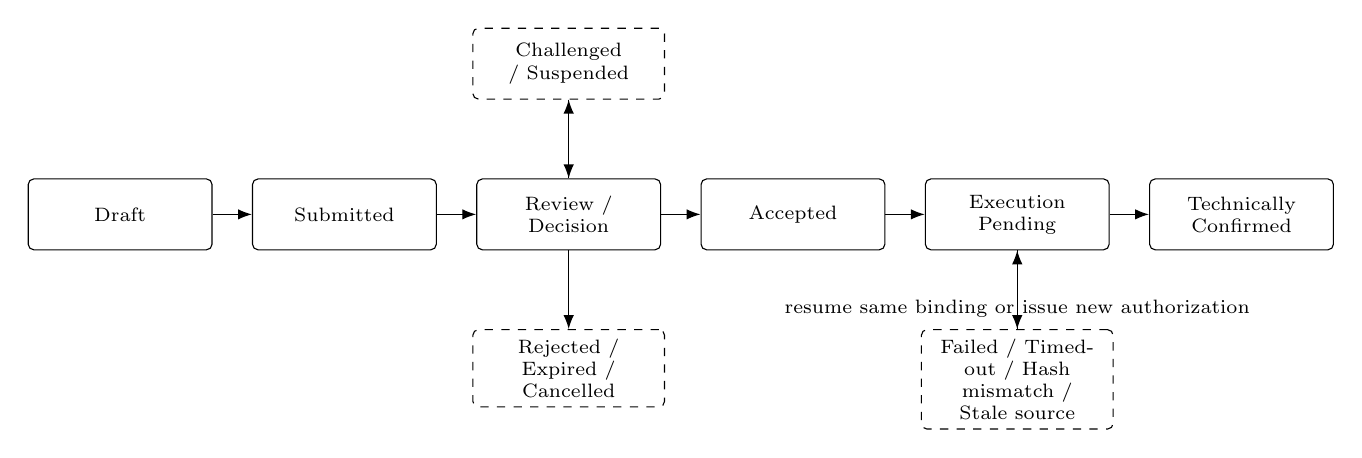
\begin{tikzpicture}[
    font=\scriptsize,
    state/.style={draw, rounded corners=2pt, align=center, text width=21mm, minimum height=9mm},
    failure/.style={draw, dashed, rounded corners=2pt, align=center, text width=22mm, minimum height=9mm},
    arrow/.style={-Latex, line width=0.45pt}
]
\node[state] (draft) {Draft};
\node[state, right=5mm of draft] (submitted) {Submitted};
\node[state, right=5mm of submitted] (review) {Review / Decision};
\node[state, right=5mm of review] (accepted) {Accepted};
\node[state, right=5mm of accepted] (pending) {Execution Pending};
\node[state, right=5mm of pending] (confirmed) {Technically Confirmed};
\node[failure, below=10mm of review] (closed) {Rejected / Expired / Cancelled};
\node[failure, below=10mm of pending] (failed) {Failed / Timed-out / Hash mismatch / Stale source};
\node[failure, above=10mm of review] (suspended) {Challenged / Suspended};
\draw[arrow] (draft) -- (submitted);
\draw[arrow] (submitted) -- (review);
\draw[arrow] (review) -- (accepted);
\draw[arrow] (accepted) -- (pending);
\draw[arrow] (pending) -- (confirmed);
\draw[arrow] (review) -- (closed);
\draw[arrow] (review) -- (suspended);
\draw[arrow] (suspended) -- (review);
\draw[arrow] (pending) -- (failed);
\draw[arrow] (failed) -- node[below,font=\scriptsize]{resume same binding or issue new authorization} (pending);
\end{tikzpicture}%
}
\caption{Coordination and execution states for a governance-bound semantic-asset lifecycle transition. Challenge and suspension are process statuses rather than terminal outcomes; acceptance and execution are distinct, and a verified receipt establishes technical confirmation.}
\label{fig:lifecycle_binding}
\end{figure*}

Figure~\ref{fig:lifecycle_binding} corrects a potentially misleading one-step interpretation of DAO governance. A proposal outcome can be final for the coordination process while the requested graph operation remains pending or fails. Conversely, an off-chain graph modification without the corresponding accepted decision and binding cannot become technically confirmed and therefore cannot pass onward to institutional confirmation.

Algorithm~\ref{lst:lifecycle_binding} summarizes the platform-independent control logic. It is a design specification, not a claim that the complete adapter and receipt protocol is implemented in the evaluated contract.

\begin{lstlisting}[
caption={Platform-independent authorization, execution, and confirmation logic},
label={lst:lifecycle_binding},
numbers=left,
numberstyle=\tiny,
stepnumber=1,
numbersep=5pt
]
process(proposal, decision):
    require decision.accepted
    require participant_eligibility_verified
    require distribution_constraint_satisfied
    require evidence_manifest_complete

    authorization = issue_scoped_authorization(proposal)
    binding = bind_exact_version_and_transition(authorization)

    if source_state_changed(binding):
        record_failure("stale-source")
        return

    receipt = request_offchain_execution(binding)

    if receipt.succeeded and
       authoritative_result_manifest_matches(receipt, binding):
        record_technical_confirmation_once(binding, receipt)
    else:
        record_failure(receipt.status)
\end{lstlisting}

The algorithm preserves four boundaries: organizational permission does not equal collective acceptance; collective acceptance does not equal execution; execution does not equal technical confirmation without result verification; and technical confirmation does not erase earlier versions or decision history. Section~\ref{sec:safeguards} supplies the additional conditions for institutional confirmation.

\subsection{Hybrid Architecture and Consolidated Requirements}
\label{sec:onchain_offchain}

The resulting architecture is hybrid because semantic data management remains off-chain while selected coordination and authorization records may be maintained on-chain. The on-chain boundary may include proposal identifiers, policy references, participation records, outcomes, authorization records, content hashes, and status events. The off-chain boundary contains RDF content, validation engines, provenance stores, canonicalization services, publication endpoints, and archival systems \cite{Hogan2021KnowledgeGraphs,Moreau2013PROV,Knublauch2017SHACL}. An execution adapter mediates between these boundaries and returns receipts; it is therefore part of the trusted and auditable system boundary rather than an invisible implementation detail.

This architecture does not require every deliberation step to occur on-chain. Institutional discussion, evidence review, and even voting may be off-chain if the selected ET-DM configuration binds their outputs to an attributable decision record. Conversely, putting a vote on-chain does not prove that the off-chain graph was validated or published. The assurance claim is therefore limited to the links and controls actually represented and implemented.

Table~\ref{tab:coord_exec_requirements} consolidates the output of this section. Coordination requirements (CRs) specialize the ET-DM Coordination layer; execution requirements (ERs) specialize its Execution layer and knowledge-graph binding. CR3 inherits ET-DM protocol parameters and adapts them per transition. CR1, CR2, CR4, CR5, and CR6 adapt coordination and Organization-to-Coordination extension points by adding semantic-asset scope, distribution, validation separation, process status, and governable administration. ER3 adapts execution guards and on-chain/off-chain function binding. ER1, ER2, ER4, ER5, and ER6 add constructs absent from the generic model: scoped authorization, separate execution states, canonicalization, attributable receipts, atomic technical confirmation, and lineage. Together these requirements provide the design specification that Section~\ref{sec:safeguards} qualifies and Section~\ref{sec:evaluation} evaluates.

\begin{table*}[t]
\caption{Consolidated ET-DM Coordination and Execution requirements}
\label{tab:coord_exec_requirements}
\centering
\renewcommand{\arraystretch}{1.12}
\setlength{\tabcolsep}{4pt}
\begin{tabular}{p{1.0cm}p{6.2cm}p{2.1cm}p{6.9cm}}
\hline
\textbf{Identifier} & \textbf{Requirement} & \textbf{Input} & \textbf{Design implication}\\
\hline
CR1 & A proposal must identify the exact asset, complete elementary or compound transition plan, expected source and target states, and evidence manifest. & OLR1--3, OLR9 & Coordination operates on versioned lifecycle transitions rather than generic RDF writes.\\
CR2 & Proposal admission and participation must derive from current role-, committee-, asset-, transition-, and distribution-scoped eligibility. & OLR4--8, OLR12 & DAO-ML organization assignments constrain ET-DM participation.\\
CR3 & Each transition must select an explicit coordination policy covering mechanism, quorum, threshold, timing, and delegation. & OLR11 & Decision semantics are transition-specific and inspectable.\\
CR4 & Validation evidence must be evaluated as a prerequisite without being treated as institutional authorization. & OLR6, OLR9 & Validation and authorization remain distinct states and permissions.\\
CR5 & Coordination must record terminal outcomes separately from attributable challenges and any resulting suspended process status. & OLR6, OLR8 & Challenges and non-success paths remain visible without being conflated with decision outcomes.\\
CR6 & Changes to roles, committees, scopes, and permissions must use governable proposal types. & OLR10 & The governance configuration cannot be changed through an unrecorded administrative bypass.\\
ER1 & An accepted decision must produce a scoped authorization record bound to one complete transition plan. & CR1--CR4 & Acceptance becomes executable authority without becoming an unrestricted write permission.\\
ER2 & The model must distinguish authorization, execution pending, execution failure, and confirmed transition states. & CR5 & A vote cannot be mistaken for completed publication.\\
ER3 & Execution must verify authorization validity, evidence integrity, expected source state, and replay protection. & OLR7--9 & Stale, altered, expired, or duplicate requests cannot confirm a transition.\\
ER4 & RDF integrity comparison must identify the canonicalization and hashing method. & OLR1, OLR9 & Graph identity does not depend on an unspecified serialization.\\
ER5 & Every off-chain attempt must return an attributable receipt containing status, an authoritative result manifest, a common commit identifier for compound plans, and failure information. & ER1--ER4 & On-chain authorization is connected to an observable semantic consequence.\\
ER6 & Technical confirmation must be atomic, idempotent, and bidirectionally traceable among asset versions, evidence, decision, binding, and receipt. & OLR1, OLR9 & Each technically confirmed state has a reconstructible governance lineage without duplicate execution.\\
\hline
\end{tabular}
\end{table*}

\subsection{Design-Stage Answer to RQ2}
At the design stage, RQ2 is answered as follows: ET-DM Coordination must bind each proposal to an exact asset, complete transition plan, evidence manifest, eligible participants, and explicit decision policy, while recording challenges and non-success outcomes separately from acceptance. ET-DM Execution must translate an accepted outcome into a scoped and expiring authorization; verify source state, evidence integrity, and replay protection; bind the authorization to the exact on-chain or off-chain operation; and require an attributable receipt whose authoritative result manifest supports atomic, idempotent, bidirectional confirmation. CR1--CR6 and ER1--ER6 operationalize this answer without asserting that every mechanism is implemented. They also expose the institutional boundary conditions---accountable identity, exceptional intervention, lawful authority, reversibility, and resistance to capture---that RQ3 must address.

\section{Institutional Extensions and Safeguards for DAOMod}
\label{sec:safeguards}

The mechanisms in Section~\ref{sec:dao_mechanisms} establish how organizationally eligible actors can form decisions and bind accepted outcomes to technically confirmed knowledge graph lifecycle transitions. Functional correctness of that chain is not sufficient for institutional acceptability. RQ3 therefore asks which safeguards and constraints must extend DAOMod to support accountability, provenance, reversibility, compliance, and resistance to governance capture. The inputs are CR1--CR6 and ER1--ER6. The output is a set of institutional safeguard requirements that qualify those mechanisms without claiming that blockchain infrastructure itself supplies institutional legitimacy.

The safeguard derivation follows three principles. First, safeguards are
attached to identifiable artifacts and transitions rather than stated as
general aspirations. Second, technical properties such as append-only
recording (adding new records without overwriting earlier ones), access
control, or hash verification are distinguished from institutional properties
such as accountable mandate, lawful authority, contestability, and independent
oversight. Third, the running case provides a demanding public-sector context,
but cross-domain transfer remains conditional on the legal, organizational,
and technical environment of each deployment. Figure~\ref{fig:accountability}
shows the safeguard overlay applied to the coordination-and-execution chain
from Section~\ref{sec:dao_mechanisms}.

\begin{figure*}[t]
\centering
\resizebox{\textwidth}{!}{%
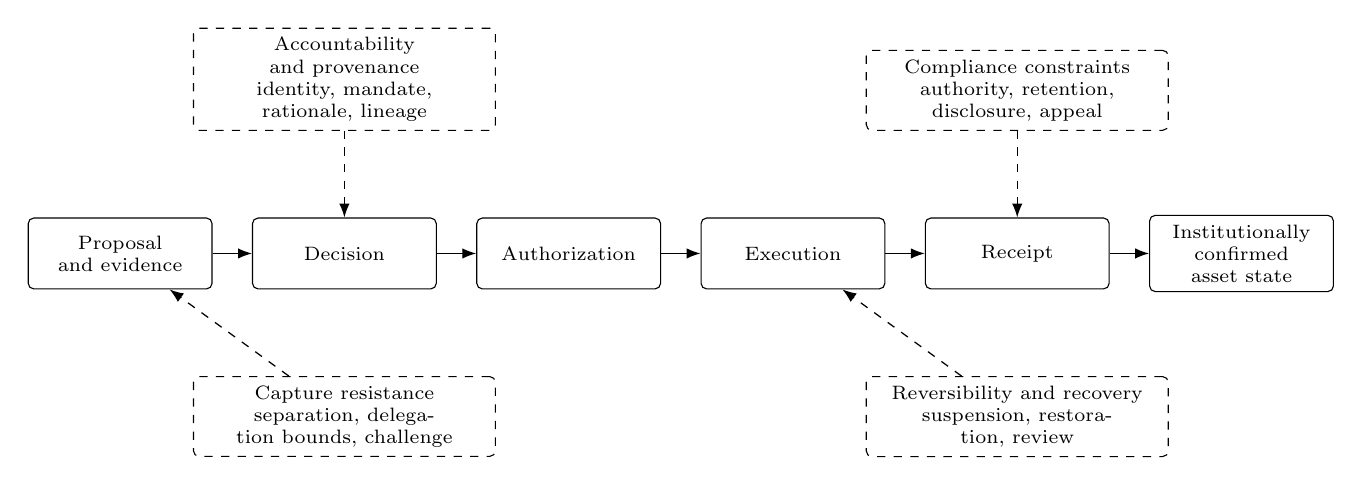
\begin{tikzpicture}[
    font=\scriptsize,
    box/.style={draw, rounded corners=2pt, align=center, text width=21mm, minimum height=9mm},
    guard/.style={draw, dashed, rounded corners=2pt, align=center, text width=36mm, minimum height=9mm},
    arrow/.style={-Latex, line width=0.45pt},
    guardarrow/.style={-Latex, dashed, line width=0.45pt}
]
\node[box] (proposal) {Proposal and evidence};
\node[box, right=5mm of proposal] (decision) {Decision};
\node[box, right=5mm of decision] (auth) {Authorization};
\node[box, right=5mm of auth] (execution) {Execution};
\node[box, right=5mm of execution] (receipt) {Receipt};
\node[box, right=5mm of receipt] (state) {Institutionally confirmed asset state};
\draw[arrow] (proposal)--(decision);
\draw[arrow] (decision)--(auth);
\draw[arrow] (auth)--(execution);
\draw[arrow] (execution)--(receipt);
\draw[arrow] (receipt)--(state);

\node[guard, above=11mm of decision] (account) {Accountability and provenance\\identity, mandate, rationale, lineage};
\node[guard, above=11mm of receipt] (compliance) {Compliance constraints\\authority, retention, disclosure, appeal};
\node[guard, below=11mm of decision] (capture) {Capture resistance\\separation, delegation bounds, challenge};
\node[guard, below=11mm of receipt] (reversal) {Reversibility and recovery\\suspension, restoration, review};
\draw[guardarrow] (account)--(decision);
\draw[guardarrow] (compliance)--(receipt);
\draw[guardarrow] (capture)--(proposal);
\draw[guardarrow] (reversal)--(execution);
\end{tikzpicture}%
}
\caption{Institutional safeguards constrain the complete governance-to-lifecycle chain rather than operating as consequences of blockchain use.}
\label{fig:accountability}
\end{figure*}

Table~\ref{tab:safeguard_traceability} identifies how the coordination and execution requirements from Section~\ref{sec:dao_mechanisms} expose the safeguard needs developed below. The mapping does not imply that one safeguard is sufficient for each risk; material risks require complementary prevention, detection, and recovery controls.

\begin{table*}[t]
\caption{Traceability from Coordination and Execution requirements to institutional safeguard dimensions}
\label{tab:safeguard_traceability}
\centering
\renewcommand{\arraystretch}{1.12}
\setlength{\tabcolsep}{4pt}
\begin{tabular}{p{2.2cm}p{4.8cm}p{4.2cm}p{5.8cm}}
\hline
\textbf{Input} & \textbf{Exposed institutional risk} & \textbf{Safeguard dimension} & \textbf{Required extension}\\
\hline
CR1, CR4, ER1 & Proposal or authorization lacks attributable rationale or adequate evidence & Accountability and provenance & Bind mandate, rationale, evidence manifest, decision, and authorization record.\\
CR2, CR3, CR5 & Eligible participants collude, dominate, censor, or prevent resolution & Capture resistance and contestability & Separation, concentration monitoring, challenge, escalation, and visible non-success outcomes.\\
CR6 & Roles, permissions, or governance policies are changed through capture or administrative bypass & Constitutional governance & Subject organizational changes to dedicated authority, review, and audit requirements.\\
ER2, ER5 & Accepted decisions remain unexecuted or failed operations are concealed & Operational accountability and recovery & Preserve pending and failure states, attributable receipts, timeouts, and escalation.\\
ER3, ER4 & Stale, altered, or improperly disclosed evidence or content is acted upon & Integrity and compliance & Verify current evidence, canonical hashes, source state, disclosure restrictions, and policy holds.\\
ER6 & Graph versions cannot be reconstructed, contested, or safely restored & Provenance and reversibility & Maintain bidirectional lineage, immutable version retention, and forward-only restoration procedures.\\
\hline
\end{tabular}
\end{table*}

\subsection{Accountability, Provenance, and Auditability}
\label{sec:accountability}

Technical transparency becomes institutional accountability only when governance actions can be related to identifiable responsibilities and mandates \cite{Schwabe2020KGTrustGovernance,Kassen2025BlockchainGovernance}. A blockchain address, signature, or committee membership proves control of a technical credential under stated assumptions; it does not by itself establish why the holder was entitled to act for an institution. The Organization-layer assignments from Section~\ref{sec:governance_requirements} must therefore be complemented by an accountable-identity reference that connects each participating actor to a role, responsible institution, mandate, and period of validity. Identity details may remain in a protected institutional registry while the governance record stores a persistent reference.

Accountability also requires an interpretable decision record. For each proposal, the system must preserve the requested asset transition, evidence manifest, applicable policy, participating roles or committees, outcome, rationale, dissent or challenge records where required, and any delegation used. These records supplement rather than duplicate W3C PROV: provenance describes entities, activities, agents, and derivations, while the governance record explains the institutional authorization associated with a transition \cite{Moreau2013PROV,Lebo2013PROVO}.

For an institutionally confirmed semantic-asset version $v$, Eq.~\ref{eq:governance_lineage} defines the minimum governance lineage:
\begin{equation}
\label{eq:governance_lineage}
\begin{aligned}
Lineage(v)=\langle&mandate,proposal,evidence,\\
&decision,authorization,binding,\\
&receipt,priorVersion\rangle.
\end{aligned}
\end{equation}
Completeness requires every element applicable to the transition to be resolvable and mutually consistent. Conversely, each accepted decision must resolve to either a receipt and confirmed consequence or an explicit pending, failed, expired, or superseded status. This bidirectional condition prevents successful graph changes from becoming detached from their authority and prevents accepted decisions from being mistaken for completed execution.

The tuple can be read as the audit trail that a reviewer follows. Starting from the published WoodHive version, the reviewer must be able to recover the prior version, execution receipt, binding, authorization, decision, evidence, proposal, and institutional mandate; following the records in the opposite direction must lead back to the same published version or to an explicit non-success status.

Records should be described as tamper-evident or append-only under the assumptions of the selected infrastructure, not as unconditionally immutable. Institutional auditability additionally requires human-readable exports, durable identifiers, clock and signer information, retention metadata, and access controls suitable for internal and external review. What is publicly visible may differ from what an authorized auditor can inspect; selective disclosure is addressed further in Section~\ref{sec:compliance}.

These extensions qualify CR1, CR4, ER1, ER5, and ER6. They also establish the evidence needed in Section~\ref{sec:evaluation}: a test or contract event can demonstrate that a field was recorded, but institutional accountability additionally requires evidence that the referenced identity, mandate, rationale, and off-chain records exist and remain interpretable.

\subsection{Forward-Only Reversibility and Exceptional Governance}
\label{sec:reversibility}

Institutional finality cannot mean that an erroneous or unlawful semantic state remains active indefinitely. At the same time, reversibility must not delete the decision and provenance history that made an earlier version authoritative. The lifecycle model therefore uses forward-only corrective transitions. For a retained version $v_k$ in state $s_k\in\{\mathit{superseded},\mathit{deprecated},\mathit{archived}\}$ and the current version $v_c$, Eq.~\ref{eq:restoration_plan} defines the compound restoration plan:
\begin{equation}
\label{eq:restoration_plan}
\begin{aligned}
&g_{restore}(v_k,v_c)=\{\\[-1mm]
&\quad (v_k,s_k,\mathit{publish},\mathit{published}),\\
&\quad (v_c,\mathit{published},\mathit{supersede},\mathit{superseded})\}.
\end{aligned}
\end{equation}
Restoration republishes the earlier version through a new proposal, decision, authorization, binding, and receipt:
\begin{equation}
\label{eq:restoration_records}
\begin{aligned}
Restore(v_k,v_c)=\langle&p_{new},d_{new},z_{new},\\
&b_{new},r_{new}\rangle,\\
g(p_{new})&=g_{restore}(v_k,v_c).
\end{aligned}
\end{equation}
Equation~\ref{eq:restoration_records} shows that restoration creates a complete
new governance chain rather than reusing the earlier authorization. The new
records explain why $v_k$ again becomes current while $v_c$ remains in the
retained history. This differs from rewinding a ledger or mapping a current
state directly to an earlier time index \cite{Moreau2013PROV,Dibowski2024TraceabilityKG}.

For example, if a later model incorrectly changes the WoodHive event and the earlier version $v_k$ is still valid, restoration does not erase the incorrect version. It creates a new proposal, decision, authorization, binding, and receipt that explain why $v_k$ becomes authoritative again.

The artifact distinguishes ordinary correction, suspension, restoration, and emergency intervention. Ordinary correction creates and governs a new candidate version. Suspension or a publication freeze temporarily prevents further activation or distribution while investigation occurs. Restoration makes a retained earlier version current through the normal binding and receipt chain. Emergency intervention permits a designated role or committee to invoke a restricted protocol when delay would create unacceptable harm. Even an emergency operation must identify the affected asset and transition, record its rationale and executor, and produce an execution receipt.

Emergency authority creates a direct capture risk and therefore requires explicit bounds: permitted operation types, asset scope, activation condition, maximum duration, delegation prohibition or restriction, mandatory notification, independent review, and an expiry or renewal rule \cite{rikken2023governance,augustin2023understanding}. Post-hoc review does not retroactively make an unlawful action legitimate; it determines whether the intervention complied with the modeled policy and what corrective action follows. Legal adequacy remains an external assessment.

\begin{figure}[t]
\centering
\resizebox{\columnwidth}{!}{%
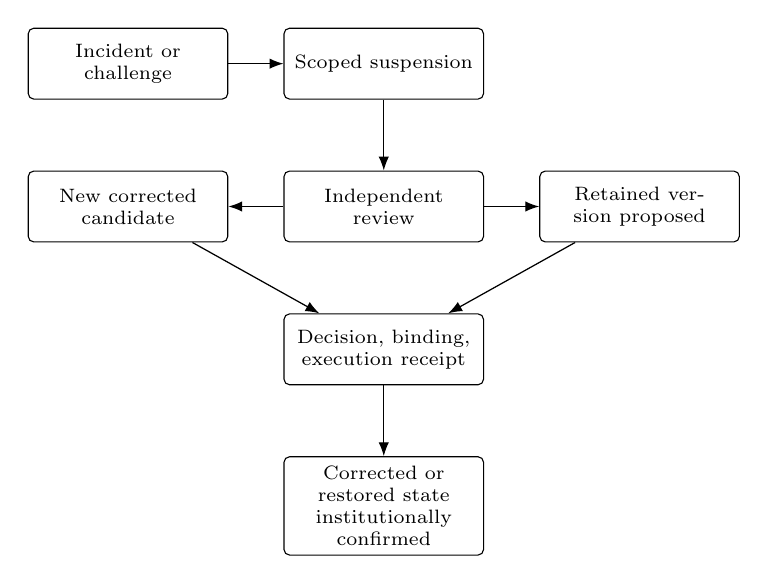
\begin{tikzpicture}[
    font=\scriptsize,
    state/.style={draw, rounded corners=2pt, align=center, text width=23mm, minimum height=9mm},
    arrow/.style={-Latex, line width=0.45pt}
]
\node[state] (incident) {Incident or challenge};
\node[state, right=7mm of incident] (suspend) {Scoped suspension};
\node[state, below=9mm of suspend] (review) {Independent review};
\node[state, left=7mm of review] (correct) {New corrected candidate};
\node[state, right=7mm of review] (restore) {Retained version proposed};
\node[state, below=9mm of review] (govern) {Decision, binding, execution receipt};
\node[state, below=9mm of govern] (confirm) {Corrected or restored state institutionally confirmed};
\draw[arrow] (incident)--(suspend);
\draw[arrow] (suspend)--(review);
\draw[arrow] (review)--(correct);
\draw[arrow] (review)--(restore);
\draw[arrow] (correct)--(govern);
\draw[arrow] (restore)--(govern);
\draw[arrow] (govern)--(confirm);
\end{tikzpicture}%
}
\caption{Forward-only exceptional governance preserves history: correction or restoration still produces a new decision, binding, and execution receipt.}
\label{fig:reversibility}
\end{figure}

Figure~\ref{fig:reversibility} shows that emergency suspension can contain harm without silently declaring another version authoritative. Confirmation still depends on the execution controls in Section~\ref{sec:lifecycle_binding}. If the adapter is unavailable or a result hash fails, the exceptional process remains visibly incomplete and proceeds through escalation rather than administrative concealment.

\subsection{Compliance and Legally Bounded Authority}
\label{sec:compliance}

DAOMod can represent and operationalize referenced institutional policies, but it cannot determine whether those policies are legally valid. Legal and regulatory obligations vary by jurisdiction, institution, semantic-asset category, and purpose of processing. This subsection therefore introduces a configurable compliance-policy reference rather than presenting one universal public-sector rule set.

For a governed transition $t$, Eq.~\ref{eq:compliance_profile} represents the compliance profile:
\begin{equation}
\label{eq:compliance_profile}
\begin{aligned}
\lambda_t=\langle&jurisdiction,mandate,retention,\\
&disclosure,appeal,hold\rangle.
\end{aligned}
\end{equation}
The profile identifies the relevant jurisdiction and institutional mandate, retention and archival rule, disclosure classification, available appeal or contestation procedure, and any preservation hold. The governance mechanism records which profile was applied and can enforce machine-checkable elements such as role eligibility, retention flags, or execution holds. Interpretation of the underlying law and validation of the profile remain responsibilities of competent institutional and legal authorities.

In ordinary language, $\lambda_t$ is the policy card attached to transition $t$. A WoodHive publication proposal might identify Estonian jurisdiction, the publishing institution's mandate, the retention period for source and graph records, who may inspect protected evidence, how the decision can be appealed, and whether an investigation currently blocks publication.

This boundary has several architectural consequences. Technical addresses must resolve to legally recognizable responsibility where required. Transfer or delegation of a permission cannot exceed the delegator's mandate. Sensitive evidence and personal information should not be placed indiscriminately on a public ledger; hashes, protected repositories, selective disclosure, or access-controlled audit interfaces may be necessary. Retention requirements may outlive a specific blockchain or software platform, so export and migration must preserve identifiers and verification data. Conversely, a preservation obligation may prohibit deletion even when an asset is no longer publicly active.

Appeal and contestation must also be represented as external or linked institutional processes rather than reduced to another token vote. A legal or administrative decision may suspend execution, require reprocessing, or initiate a new corrective proposal. Such intervention enters the same accountable binding and receipt chain while deriving its authority from the referenced mandate, not from blockchain consensus. Accordingly, DAO authorization operationalizes institutional authority; it does not create legal authority \cite{Atzori2017BlockchainGovernance,Kassen2025BlockchainGovernance,Schwabe2020KGTrustGovernance}.

The evaluation can therefore verify whether a compliance reference, hold, disclosure classification, or authorized override is represented and enforced. It cannot establish general legal compliance or institutional suitability without jurisdiction-specific expert assessment and deployment evidence.

\subsection{Capture Resistance and Governance-Failure Safeguards}
\label{sec:resilience}

The explicit mechanisms in Sections~\ref{sec:governance_requirements} and~\ref{sec:dao_mechanisms} make governance behavior inspectable, but they do not eliminate strategic or operational failure. Relevant threats include concentration of authority, collusion, conflicting role assignments, delegation chains, low participation, quorum manipulation, proposal censorship, decision deadlock, abuse of emergency powers, compromised execution adapters, and selective non-execution of accepted decisions \cite{Hassan2021DAO,Han2025DAOReview,Weidener2026Metagovernance}.

Safeguards must be attached to the part of the chain where the threat occurs. Separation-of-duty and incompatibility constraints limit one actor's ability to propose, validate, authorize, and execute the same critical transition. Committee composition and, where appropriate, institution-level representation prevent nominally different accounts from disguising one controlling organization. Delegation is bounded by scope and time and remains visible in the decision record. Challenge windows, dissent records, and proposal-status transparency make censorship and disputed outcomes detectable. Concentration and participation indicators can trigger review, but their thresholds are deployment parameters rather than universal constants.

Liveness requires complementary controls. Proposals must reach an explicit outcome or escalation state instead of remaining silently unresolved. Quorum failure, executor timeout, and missing receipts trigger defined escalation or re-proposal procedures. Adapter identities, software versions, and receipts support investigation of compromised or selectively non-performing executors. Emergency mechanisms are monitored as high-risk governance actions and remain subject to the bounds and review requirements in Section~\ref{sec:reversibility}.

Safeguard coverage should not be represented merely by assigning one mitigation to each failure mode. For every material threat $f$, Eq.~\ref{eq:threat_coverage} identifies prevention, detection, and recovery controls together with residual risk:
\begin{equation}
\label{eq:threat_coverage}
\begin{aligned}
Coverage(f)=\langle&Prevent_f,Detect_f,\\
&Recover_f,Residual_f\rangle.
\end{aligned}
\end{equation}
Adequacy is a claim to be supported by threat assumptions and evaluation evidence. The mere fact that at least one of $Prevent_f$, $Detect_f$, or $Recover_f$ is non-empty does not establish adequacy. This formulation also prevents a transparency mechanism from being presented as prevention when it only improves ex-post detection.

Thus, listing a control does not establish that a threat is adequately managed. For the threat that one actor controls the WoodHive transition, separation of duties may prevent concentration, authority monitoring may detect it, and suspension plus reassignment may support recovery; any remaining ability to collude is recorded as residual risk.

The predicate in Section~\ref{sec:lifecycle_binding} establishes technical confirmation only. Let $\Gamma_{conf}(b)$ be the complete, resolved set of safeguards required for confirmation under the transition, compliance, distribution, and exceptional-status policies; let $PolicyResolved(b)$ mean that those policies and their applicable checks are identifiable; and let $Passed(g_s,b,r)$ mean that safeguard $g_s$ has a recorded satisfactory result under the modeled policy. Equation~\ref{eq:safeguard_gate} defines the safeguard gate:
\begin{equation}
\label{eq:safeguard_gate}
\begin{aligned}
SafeguardGate(b,r)\iff{}& PolicyResolved(b)\\
&\land\forall g_s\in\Gamma_{conf}(b):\\
&\qquad Passed(g_s,b,r),
\end{aligned}
\end{equation}
and Eq.~\ref{eq:institutional_confirmation} defines the stronger status:
\begin{equation}
\label{eq:institutional_confirmation}
\begin{aligned}
&InstitutionallyConfirmed(b,r)\\
&\quad\iff TechnicalConfirmed(b,r)\\
&\qquad\land SafeguardGate(b,r).
\end{aligned}
\end{equation}
Safeguards that protect execution itself---a valid mandate, policy holds, evidence-disclosure permission, and required decentralized participation---must be checked at admission and included in the admission record; result-dependent safeguards are checked against the receipt. For a critical transition, $Passed$ includes recorded satisfaction of $Distributed(t)$ and $DecentralizedDecision(p,\kappa_t)$. Only an institutionally confirmed plan may establish the artifact's authoritative lifecycle state: publication is staged until the gate passes, rather than exposed authoritatively and assessed afterward. Continuing monitoring and any mandated independent post-hoc review remain explicit obligations and may trigger suspension or a new corrective transition; they are not silently treated as already completed. $InstitutionallyConfirmed$ means confirmed under the modeled institutional policy, not that the policy or action has thereby been proven legally valid.

The two predicates distinguish faithful technical completion from satisfaction of modeled institutional checks. In the WoodHive case, the publication service may correctly stage the approved graph content, satisfying $TechnicalConfirmed$, while the transition still fails $SafeguardGate$ because a result-dependent check is unsatisfied. Only when both predicates hold may the staged graph become authoritative. A mandate expiry or preservation hold is checked earlier at admission and therefore prevents execution rather than invalidating it afterward.

Listing~\ref{lst:safeguard_gate} specifies where the principal safeguards intercept the coordination-and-execution process. It is intentionally platform-independent: the checks may be distributed across smart contracts, institutional identity services, protected evidence repositories, execution adapters, and human review procedures.

\begin{lstlisting}[
caption={Platform-independent institutional safeguard gate},
label={lst:safeguard_gate},
numbers=left,
numberstyle=\tiny,
stepnumber=1,
numbersep=5pt
]
applySafeguards(proposal, decision, binding, receipt):
    require accountable_mandate(proposal.initiator)
    require applicable_compliance_profile(proposal.transition)
    require evidence_access_and_retention_permitted()
    require separation_and_delegation_constraints_hold()
    require structural_and_realized_distribution_hold()

    if proposal.is_exceptional:
        require emergency_scope_and_expiry_valid()
        schedule_independent_review()

    require lineage_complete(proposal, decision, binding)

    if receipt.missing or receipt.failed:
        record_and_escalate_execution_failure()
        return NOT_CONFIRMED

    require lineage_complete(binding, receipt, resulting_version)
    monitor_concentration_and_non_execution()
    return MODELED_SAFEGUARD_GATE_SATISFIED
\end{lstlisting}

The successful return supplies the recorded result used by $SafeguardGate$; it does not equate that gate with legal compliance or general institutional suitability. Competent authorities and deployment-specific evaluation remain necessary.

Table~\ref{tab:institutional_safeguards} consolidates the safeguard requirements (SGs) developed for RQ3. SG1 adapts roles and permissions while adding mandate and institutional-identity binding. SG4, SG5, SG10, and SG11 adapt lifecycle, permission, delegation, eligibility, and participation constructs while adding institutional constraints. SG2, SG3, SG6, SG7, SG8, SG9, and SG12 add elements absent from the generic model: cross-layer lineage, rationale and dissent records, exceptional review, compliance references, protected-evidence metadata, external-decision links, and explicit escalation states. These requirements are the final design input to Section~\ref{sec:evaluation}; they are not claims that the evaluated contract implements every safeguard.

\begin{table*}[t]
\caption{Consolidated institutional safeguard requirements}
\label{tab:institutional_safeguards}
\centering
\renewcommand{\arraystretch}{1.12}
\setlength{\tabcolsep}{4pt}
\begin{tabular}{p{1.0cm}p{6.1cm}p{2.2cm}p{6.9cm}}
\hline
\textbf{Identifier} & \textbf{Safeguard requirement} & \textbf{Input} & \textbf{Required evidence or enforcement point}\\
\hline
SG1 & Resolve technical participants to accountable roles, institutions, mandates, and validity periods. & CR2, ER1 & Protected identity/mandate registry and persistent governance reference.\\
SG2 & Preserve complete bidirectional lineage among proposal, evidence, decision, authorization, binding, receipt, and asset version. & CR1, CR4, ER5--6 & Resolvable identifiers and consistency checks in both directions.\\
SG3 & Preserve interpretable rationale, challenges, delegation, and human-readable audit exports. & CR3--5 & Decision metadata, dissent records, timestamps, and exportable audit representation.\\
SG4 & Implement correction and restoration as forward-only governed transitions without deleting prior history. & ER2, ER6 & New proposal-to-receipt chain referencing the retained or corrected version.\\
SG5 & Bound emergency authority by operation, asset scope, trigger, duration, delegation, and expiry. & CR2--3, ER1 & Explicit exceptional policy and rejected out-of-scope or expired actions.\\
SG6 & Require notification and independent post-hoc review of exceptional interventions. & CR5, ER5 & Review record, outcome, and any resulting corrective proposal.\\
SG7 & Associate each transition with a jurisdiction- and mandate-specific compliance-policy reference. & CR1, CR3 & Recorded policy identifier and competent institutional approval.\\
SG8 & Enforce retention, preservation-hold, disclosure, and selective-access metadata without exposing protected content on-chain. & CR4, ER3--4 & Policy flags, protected evidence repository, and controlled audit access.\\
SG9 & Link appeal, contestation, and legally mandated intervention to suspension or corrective governance procedures. & CR5, ER2 & External decision reference and accountable follow-on transition.\\
SG10 & Enforce separation of duties, incompatible assignments, and bounded delegation for critical transitions. & CR2--3, CR6 & Admission checks and visible assignment/delegation history.\\
SG11 & Monitor authority concentration, participation, challenges, and emergency-power use under deployment-specific thresholds. & CR2--5 & Indicators, alerts, review triggers, and documented residual risk.\\
SG12 & Detect and escalate deadlock, censorship, executor timeout, missing receipt, and selective non-execution. & CR5, ER2, ER5 & Explicit failure states, timeouts, escalation records, and attributable executor status.\\
\hline
\end{tabular}
\end{table*}

\subsection{Design-Stage Answer to RQ3 and Provisional Synthesis}
At the design stage, RQ3 is answered through four groups of safeguards.
First, technical identities must resolve to time-bounded institutional
mandates, and the resulting records must preserve bidirectional lineage,
rationale, dissent, delegation, and human-readable audit evidence. Second,
correction and restoration must be forward-only governed transitions, while
emergency powers must remain bounded and reviewable. Third, each transition
must carry an applicable jurisdiction- and mandate-specific compliance
reference, protect sensitive evidence, and connect appeals or external
decisions to corrective procedures. Finally, the design must enforce
separation of duties and bounded delegation while monitoring concentration,
liveness, and non-execution. SG1--SG12 operationalize these safeguards. They
make institutional obligations and residual risks inspectable, but do not
establish legal validity or stakeholder acceptance.

Taken together, the design-stage answers to RQ1--RQ3 provide a provisional answer to the MRQ: DAOMod can be specialized for institutional knowledge graph lifecycles by organizing authority around versioned semantic-asset transitions, binding collective decisions to exact executable operations and attributable result manifests, and qualifying technical confirmation with explicit institutional safeguards. This is a design proposition whose internal traceability is established in Sections~\ref{sec:governance_requirements}--\ref{sec:safeguards}; its implementation coverage and practical adequacy remain matters for evaluation.
\section{Evaluation}
\label{sec:evaluation}

This section evaluates the proposed decentralized governance and
authorization artifact with respect to the research questions and
governance requirements derived in
Sections~\ref{sec:governance_requirements}--\ref{sec:safeguards}.
Following a design-science perspective~\cite{hevner2004design},
we assess the artifact in its intended problem context rather than
benchmark it against alternative implementation platforms.

Two related but non-equivalent artifacts must be distinguished. The
\emph{design artifact} is the platform-independent specialization expressed by
OLR1--OLR12, CR1--CR6, ER1--ER6, and SG1--SG12. The \emph{evaluated
implementation} is the available smart-contract prototype against which those
requirements are mapped. Section~\ref{sec:evaluation} therefore performs both
a complete traceability assessment of the design requirements and a narrower
behavioral evaluation of the mechanisms present in the prototype. A
requirement specified by the design is not treated as implemented unless the
reported source and execution evidence supports that conclusion.

The object of the baseline evaluation is the on-chain governance layer alone, not the
hybrid architecture described in
Sections~\ref{sec:smart_contracts}--\ref{sec:safeguards}. The evaluation
examines whether lifecycle transitions recorded on-chain are authorized,
attributable, and auditable. It does not exercise the off-chain
components on which that architecture depends: the RDF stores holding the
semantic assets, the validation pipelines producing the results the
contracts record, the publication services that write to the
decentralized knowledge graph, or the provenance records those services
emit. Nor does it establish that an off-chain action faithfully reflects
the on-chain decision authorizing it: no execution receipt is returned to
the baseline contracts, and the correspondence between the hash of an approved
graph and the asset identifier of the published one is stored but never
verified. What the baseline establishes is therefore the feasibility of
contract-level authorization, not end-to-end governance of a knowledge
graph lifecycle.

The running case is a high-trust, regulated setting in which
unauthorized or untraceable lifecycle transitions carry legal and
institutional consequences. The evaluation therefore interprets each
situation through the hypothetical WoodHive employment graph introduced in
Section~\ref{sec:runningcase}: the graph is submitted, validated, approved,
published, reprocessed after a model change, or left unresolved after a
failed decision. This common example connects the contract operations to
the semantic consequences that motivate the requirements.

A separate supplemental episode, reported in
Section~\ref{sec:publication_episode}, extends the executed boundary to a
local RDF store and a publication adapter. It uses a new bounded contract and
the existing committee procedure, not a silent modification of the evaluated
baseline. The 36-row crosswalk and historical coverage figures retain their
original meaning.

The evaluation proceeds through the baseline assessment and the supplemental
local integration episode.
Section~\ref{sec:eval_method} sets out the evaluation design, the
evidence boundary, and the assessment criteria.
Section~\ref{sec:capability_assessment} reports requirement coverage
for the mechanisms exercised in the evaluated build and identifies
those that are specified in the design sections but not executed.
Section~\ref{sec:artifact_availability} specifies the reproducibility
package and immutable artifact revision.
Section~\ref{sec:discussion} relates the findings to the research
questions and discusses limitations and threats to validity.

\subsection{Evaluation Design and Scope}
\label{sec:eval_method}

The evaluation follows an ex-post design-science strategy: the
artifact is examined after construction against the governance
requirements derived in
Sections~\ref{sec:governance_requirements}--\ref{sec:safeguards}. The
object of evaluation is the smart-contract implementation of the
governance layer---the role and permission registry, the
semantic-asset lifecycle registry, the collective-decision contract,
and the optimistic-governance contract---together with its automated
test suites. The evaluated revision is the immutable commit
\texttt{3c55c6903fe6fb38177889e22adf9639f8b9cda5}.\footnote{Reviewer entry point:
\url{https://github.com/alexbafana/MKM-POL21-2025/tree/3c55c6903fe6fb38177889e22adf9639f8b9cda5/reproducibility/paper-b}.}
In an optimistic procedure, a proposal may proceed after a declared challenge
period unless an eligible participant objects. This contrasts with the
separate committee procedure, which requires an affirmative vote.

The declared semantic-processing stages and the executed evaluation stages are
different. NLP, named-entity recognition, LLM classification, EMTAK linking,
RDF generation, semantic validation, RDF-store publication, and institutional
review are declared components of the running-case environment and proposed
hybrid architecture; none is executed in the baseline evaluation. The baseline executed stages
are contract compilation, fixture deployment, contract tests, instrumented
Solidity coverage, and manifest/crosswalk validation. The omitted stages are
not silently treated as successful: the evaluated pilot contains no off-chain
services with which to execute them, and population-level semantic or
institutional claims would require a labeled dataset, domain review, and live
multi-organization deployment that the study does not provide.

The evaluated contract names its registry states \emph{Created}, \emph{Validated}, \emph{Approved}, and \emph{Published}. These names are retained when reporting implementation behavior. They differ from the design model in Section~\ref{sec:lifecycle}, where a created version is a candidate and authorization is deliberately modeled as a decision status rather than as an asset state. The evaluation makes this mismatch explicit because an ``Approved'' registry value can otherwise blur the distinction between institutional authorization and a semantic-asset lifecycle state.

Four evaluation questions (EQ1--EQ4) make the inference from evidence to findings
explicit. Table~\ref{tab:evaluation_questions} states both the evidence used
and the limit of each answer. EQ1 asks for systematic design-to-implementation
traceability; EQ2 asks whether the represented controls behave correctly on
the tested paths; EQ3 asks whether the executed evidence is broad enough to
expose untested contract structure and can be rerun from a clean checkout; and
EQ4 asks which claims remain unsupported despite successful execution.

\begin{table*}[t]
\centering
\caption{Evaluation questions, evidence, and decision criteria}
\label{tab:evaluation_questions}
\renewcommand{\arraystretch}{1.1}
\footnotesize
\begin{tabular}{@{}c p{5.0cm} p{5.2cm} p{5.5cm}@{}}
\toprule
\textbf{ID} & \textbf{Evaluation question} & \textbf{Evidence} & \textbf{Decision criterion and inferential limit} \\
\midrule
EQ1 & To what extent does the evaluated build represent and exercise each of OLR1--OLR12, CR1--CR6, ER1--ER6, and SG1--SG12? & Contract state, functions, guards, and events; test paths; 36-row crosswalk. & Assign E, P, or N to every complete requirement using the rule below. The result is implementation coverage, not legal or institutional conformance. \\
EQ2 & Do represented authorization, lifecycle-ordering, decision, and failure controls distinguish intended behavior from plausible violations? & Positive paths and negative, boundary, and bypass tests, including tests labelled \texttt{GAP:}. & A claim is supported only for the exercised configuration and reachable paths. A passing \texttt{GAP:} test is negative evidence when it demonstrates a missing safeguard. \\
EQ3 & Is the executable evidence reproducible and structurally broad within the declared contract boundary? & Clean execution of all tests, Solidity statement/branch/function/line coverage, manifest validation, lockfile, and continuous-integration workflow. & The clean command must reproduce the expected counts. Coverage measures exercised code breadth; it does not establish requirement satisfaction. \\
EQ4 & Which design and institutional claims remain outside the evidence boundary? & Missing enforcement points, incomplete bindings, excluded off-chain services, and the absence of independent organizational or legal evaluation. & Unsupported claims are reported as P or N, or explicitly excluded; passing tests cannot be generalized to end-to-end or institutional suitability. \\
\bottomrule
\end{tabular}
\end{table*}

Five governance situations drawn from the running case structure the
assessment. Situation 1 (S1), governance approval, concerns the transition from a
validated to an approved graph state, which authorizes publication
without performing it. Situation 2 (S2), lifecycle update authorization, concerns the
ordered sequence from submission through validation and approval to
publication, and so covers the approved-to-published transition that
completes it. Situation 3 (S3), model-driven reprocessing, concerns the creation of a
further graph version under a changed model version; whether the
reprocessed content corrects an earlier extraction error is a property
of the off-chain pipeline and is not observable on-chain. Situation 4 (S4), forward-only restoration,
represents the requirement that a semantic asset be restorable to a
previously published state. Situation 5 (S5), governance deadlock, concerns the
outcome of a decision procedure that fails to reach quorum within its
declared voting period. These five situations were selected because each turns on an
authorization decision that the contracts are meant to enforce, and
because together they sample successful and unsuccessful paths through the lifecycle model of
Section~\ref{sec:lifecycle}. They do not span the governance concerns
raised in Sections~\ref{sec:governance_requirements}--\ref{sec:safeguards}
as a whole. Deprecation and archival are omitted because no
corresponding transition exists in the evaluated build; emergency
intervention is omitted because SG5--SG6 specify its constraints and review
obligations but the evaluated build implements no exceptional transition or
policy. Capture, collusion and trust erosion
are addressed in Section~\ref{sec:safeguards} as properties of the
institutional arrangement rather than of a single transition, and
establishing them would require the participation of independent
organizations that this evaluation does not have. End-to-end publication
is excluded by the scope stated above. The situations therefore
illustrate the governance layer in operation; systematic coverage is
carried by the requirement-level mapping in
Section~\ref{sec:capability_assessment}, which reports every requirement
derived in the design phase, including those with no implementation.

The unit of analysis for EQ1 is one complete platform-independent
requirement, rather than one test or function. For each requirement $r$, the
authors (1) read all clauses of the requirement, (2) identified candidate
state, functions, guards, events, and tests, (3) inspected positive, negative,
boundary, and bypass paths, (4) assigned the most conservative supported
status, (5) recorded the evidence paths and the unmet clause, and (6) checked
identifier uniqueness and aggregate counts mechanically. Let $C_b(r)$ be the
material clauses of $r$ that are observable within the declared contract
boundary, $H(r)\subseteq C_b(r)$ the clauses for which a reachable
representation or enforcement point was found, and $D(r)$ indicate that the
intended behavior is distinguished by execution from a plausible failure
where such a distinction applies. The coding rule is
\begin{equation}
\label{eq:coverage_status}
s(r)=
\begin{cases}
\mathrm{E}, & H(r)=C_b(r)\ \land\ D(r),\\
\mathrm{N}, & H(r)=\emptyset,\\
\mathrm{P}, & \text{otherwise}.
\end{cases}
\end{equation}
Thus, E denotes directly exercised support for all contract-observable clauses,
P denotes at least one represented clause but a missing clause, binding,
scope, or distinguishing execution, and N denotes no corresponding reachable
implementation. The rule deliberately biases ambiguous cases toward P or N.
It does not turn an E into evidence of legal adequacy. The coding is an
auditable authorial interpretation; no independent second coder or inter-rater
agreement is claimed.

Assessment criteria are operationalized as checkable conditions.
\emph{Authorization enforceability} requires that a guarded transition
succeed for an authorized caller and revert---terminate without applying a
state change---for an unauthorized one.
\emph{Accountability} requires that each executed transition record
the acting party. \emph{Auditability} requires that each governed
transition emit a durable record identifying the decision, the actor,
and the affected asset. \emph{Lifecycle traceability} requires that
the sequence of transitions applied to an asset be reconstructible
from those records. \emph{Reversibility} requires that a published
state be restorable under authorization. \emph{Termination under
quorum failure} requires that a decision procedure which does not
reach quorum within its declared voting period arrive at a defined
terminal state from which it cannot be executed. This is narrower than
the resilience property specified in Section~\ref{sec:resilience},
which additionally requires that a stalled procedure activate an
escalation path; that mechanism is not implemented in the evaluated
build, so it is not exercised and is recorded as absent. Compliance is addressed by design
in Section~\ref{sec:compliance} and is likewise outside what contract
execution can establish: whether an institution meets its retention,
disclosure, and appeal obligations is a legal determination, and
establishing it would require a structured requirements walkthrough or
review by legal experts rather than test execution. RQ3 is accordingly
evaluated in its technically observable dimensions: accountability,
traceability, forward-only history, and failure handling. The coverage
assessment can still determine whether compliance references,
protected-evidence metadata, exceptional policies, and review hooks are
represented in the implementation; it cannot determine whether those
mechanisms are legally adequate. Restoration is reported as unimplemented,
and legal compliance remains outside the inferential scope of contract tests.

Evidence is drawn from four sources and supports claims of different
strength. Contract sources establish \emph{existence and reachability}: which
state, authorization checks, and guards are present. Executed tests establish
\emph{observed behavior} under their constructed conditions. Instrumented
coverage establishes \emph{structural breadth} within the declared source
boundary, not conformance. Finally, the machine-readable crosswalk exposes the
\emph{authorial interpretation} connecting that technical evidence to each
platform-independent requirement. A higher source-coverage percentage cannot
upgrade P or N to E, and a passing test named after a requirement cannot do so
unless all contract-observable clauses meet the rule in
Eq.~\ref{eq:coverage_status}.

These sources provide no evidence of \emph{institutional suitability}:
neither legal compliance, nor organizational legitimacy of the modeled roles
and decision rights, nor operational suitability under institutional workload
follows from source inspection or test execution. The test suites and
crosswalk were produced by the authors alongside the artifact, so they reflect
the properties the authors set out to demonstrate and cannot rule out untested
failure modes or interpretation bias. These limits apply especially to RQ3,
for which the evaluation can inspect event-level attribution and traceability
but cannot establish legal compliance or institutional legitimacy.

\subsection{Requirements Coverage and Verification Results}
\label{sec:capability_assessment}

This subsection assesses the governance artifact against the
requirements identified during the design phase. The assessment
proceeds through the five governance situations introduced in
Section~\ref{sec:eval_method}. Following the distinction drawn there,
what is reported below is the existence of each mechanism and the
outcome of executing it; conformance to the corresponding institutional
requirement rests on the mapping between the two, which is stated
explicitly so that it can be inspected rather than assumed.

The five situations resolve as follows. S1 and S2 are exercised: the
guarded transitions and the constraints on their order are covered by
executed tests. S3 is exercised as model-driven reprocessing: a further version is
created, carries its own model version, and starts in the Created state
rather than inheriting the predecessor's approval. S5 is exercised: a proposal
that fails to reach quorum within its voting period reaches a terminal
defeated state and cannot be executed. S4 is specified in
Section~\ref{sec:reversibility} but not implemented in the evaluated
build, and is therefore reported as such rather than exercised.

Two complementary mappings are required. Table~\ref{tab:coverage}
first preserves the implementation test suite's own requirement-to-test
mapping. It records, for each implementation requirement, the mechanism,
the contract function implementing that mechanism, the test
exercising it, and the resulting status. The identifiers R1.x, R2.x, and
R3.x are the implementation test suite's requirement identifiers; they are
distinct from the platform-independent OLR, CR, ER, and SG identifiers
developed earlier and therefore cannot by themselves establish coverage of
the design artifact. Status ``E'' means that an executed test exercised the
mechanism, whereas ``N'' means that the design specifies the requirement but
the evaluated build does not implement it. The implementation also uses a
time-limited identity attestation, meaning a recorded claim about a
participant's identity or eligibility. Its nine challenge-response checks
are termed multi-factor challenge-set self-sovereign identity authentication
(MFSSIA) in the implementation.

\begin{table*}[t]
\centering
\caption{Legacy implementation-requirement mapping at evaluated commit \texttt{3c55c690\ldots}: E denotes an exercised mechanism and N denotes no corresponding implementation.}
\label{tab:coverage}
\renewcommand{\arraystretch}{1.15}
\footnotesize
\begin{tabular}{@{}l p{4.1cm} p{5.5cm} c c c@{}}
\toprule
\textbf{Requirement} & \textbf{Mechanism} & \textbf{Contract / function} &
\textbf{Tests} & \textbf{Status} & \textbf{Qualification} \\
\midrule
\multicolumn{6}{@{}l}{\textit{RQ1 --- Governance roles, permissions, and decision rights}} \\
\addlinespace[2pt]
R1.3 & Actions gated by per-role permission set & \texttt{MKMPOL21.has\_permission} & 9 & E & \\
R1.5 & Permission bit 28 checked on proposal creation & \texttt{Consortium.propose} & 4 & E & \\
R1.6 & Permission bit 29 checked on veto & \texttt{Consortium.vetoProposal} & 7 & E & \\
R1.7 & Revocation applies to all holders of the role & \texttt{MKMPOL21.revokePermission}, \texttt{revokeRole} & 2 & E & \\
\addlinespace[3pt]
\midrule
\multicolumn{6}{@{}l}{\textit{RQ2 --- Governance mechanisms and authorization semantics}} \\
\addlinespace[2pt]
R2.5 & Version derived on-chain per dataset and year & \texttt{GADataValidation.submitRDFGraph} & 5 & E & \\
R2.6 & Model version recorded with each version & \texttt{submitRDFGraph} & 5 & E & \\
R2.7 & Syntactic and semantic results recorded separately & \texttt{markRDFGraphValidatedWithDetails} & 8 & E & a \\
R2.8 & Quorum-based voting, proposal and vote rights gated & \texttt{ValidationCommittee.propose}, \texttt{castVote} & 7 & E & \\
R2.9 & Challenge period elapsed before execution & \texttt{Consortium.execute} & 4 & E & \\
R2.10 & Quorum as fraction of voting power at snapshot & \texttt{GovernorVotesQuorumFraction} & 5 & E & \\
R2.11a & Optimistic proposal drives Created\,$\rightarrow$\,Validated & \texttt{Consortium.execute} $\rightarrow$ \texttt{markRDFGraphValidated} & 3 & E & \\
R2.11b & Committee vote drives Validated\,$\rightarrow$\,Approved & \texttt{ValidationCommittee} $\rightarrow$ \texttt{approveRDFGraph} & 6 & E & b \\
R2.12 & --- & --- & --- & N & c \\
R2.13 & --- & --- & --- & N & \\
R2.14 & --- & --- & --- & N & \\
\addlinespace[3pt]
\midrule
\multicolumn{6}{@{}l}{\textit{RQ3 --- Safeguards: accountability and traceability}} \\
\addlinespace[2pt]
R3.1 & Event carries the acting contract address & \texttt{RDFGraphValidated}, \texttt{RDFGraphApproved} & 2 & E & \\
R3.2 & Submitter, timestamp, hash and version stored & \texttt{getRDFGraphBasicInfo}, \texttt{getRDFDocument} & 4 & E & \\
R3.3 & Attestation stored on onboarding, valid one year & \texttt{onboard\_*\_with\_attestation} & 6 & E & d \\
R3.5 & Eight of nine MFSSIA identity challenges required & \texttt{submitRDFDocument} & 10 & E & \\
R3.6 & --- & --- & --- & N & \\
R3.7 & --- & --- & --- & N & \\
R3.11 & Guards applied on every reachable execution path & \texttt{Consortium.execute}, \texttt{relay} & 4 & E & e \\
\bottomrule
\end{tabular}

\vspace{3pt}
\begin{minipage}{\textwidth}
\footnotesize
An exercised status records test execution, not proof that the corresponding
institutional requirement is satisfied. The qualification column marks rows
where execution revealed a material limitation. Test counts
are tests naming the requirement; the full mapping is in the repository.\\
\textsuperscript{a}Approval and publication gate on the syntactic result only.\quad
\textsuperscript{b}Possible through the committee but not enforced: the registry authorizes approval by permission check.\quad
\textsuperscript{c}Content hash and published asset identifier are both stored; no correspondence is verified.\quad
\textsuperscript{d}The attestation is recorded and expires, but is not verified at submission.\quad
\textsuperscript{e}The consortium quorum is configured at zero.
\end{minipage}
\end{table*}

Tables~\ref{tab:olr_coverage}, \ref{tab:crer_coverage}, and
\ref{tab:sg_coverage} provide the second mapping: they assess every
Organization, Coordination, Execution, and Safeguard requirement in the design artifact against the
source and test evidence summarized in Table~\ref{tab:coverage}. ``E'' denotes
directly exercised support for the stated requirement within the implemented
scope, ``P'' denotes partial support because one or more required clauses or
bindings are absent, and ``N'' denotes no corresponding implementation.
These are coverage categories, not quality scores or claims of institutional
conformance. In particular, an exercised mechanism may still have the
qualification reported in Table~\ref{tab:coverage}.

\begin{table*}[t]
\centering
\caption{Design-to-implementation coverage of the Organization-layer requirements: E denotes direct exercised support, P partial support, and N no reachable implementation.}
\label{tab:olr_coverage}
\renewcommand{\arraystretch}{1.08}
\scriptsize
\begin{tabular}{@{}c c p{13.8cm}@{}}
\toprule
\textbf{ID} & \textbf{Status} & \textbf{Evidence and boundary} \\
\midrule
OLR1 & E & Dataset/year versions, content hashes, and individually addressable records are created and queried in executed tests. \\
OLR2 & P & Registry states and guarded forward edges are represented, but \emph{Approved} conflates authorization with asset state; restoration, deprecation, archival, and supersession are absent. \\
OLR3 & N & Permission bits are role-wide rather than jointly scoped to asset class and transition type. \\
OLR4 & P & Named roles and action permissions are represented, but the evaluated allocation does not preserve independent lifecycle responsibilities. \\
OLR5 & E & Consortium and validation-committee contracts represent identifiable collective bodies and exercise their membership-based procedures. \\
OLR6 & P & Submission, validation, approval, publication, proposal, and veto are separately guarded, but the complete specialized permission vocabulary is not represented. \\
OLR7 & N & No joint role/committee--asset--transition permission relation is enforced. \\
OLR8 & N & One role can submit, validate, and approve; delegation and incompatible-assignment bounds are not enforced. \\
OLR9 & P & Hash, model version, and separate validation results are stored, but required evidence is not transition-scoped and semantic failure does not block approval or publication. \\
OLR10 & N & Role and permission administration is callable directly rather than modeled as a governed proposal and transition. \\
OLR11 & N & Two coordination procedures exist, but a transition carries no explicit reference to its applicable policy. \\
OLR12 & N & Independent-principal distribution is neither represented nor enforced; test accounts are controlled by one party. \\
\bottomrule
\end{tabular}
\end{table*}

\begin{table*}[t]
\centering
\caption{Design-to-implementation coverage of the Coordination and Execution requirements using the E/P/N assessment rule.}
\label{tab:crer_coverage}
\renewcommand{\arraystretch}{1.08}
\scriptsize
\begin{tabular}{@{}c c p{13.8cm}@{}}
\toprule
\textbf{ID} & \textbf{Status} & \textbf{Evidence and boundary} \\
\midrule
CR1 & P & Proposals can target lifecycle calls and graph versions, but no complete transition plan with expected states and evidence manifest is recorded. \\
CR2 & P & Proposal, vote, and veto admission use current role permissions, but asset-, transition-, distribution-, mandate-, and attestation-scoped eligibility is incomplete. \\
CR3 & P & Voting, quorum, timing, and challenge periods are executable, but policy selection is hard-coded rather than referenced per transition and the consortium quorum is zero. \\
CR4 & P & Validation and approval are distinct operations, but only syntactic success gates later transitions and the evidence requirement is incomplete. \\
CR5 & P & Defeat and veto/challenge behavior are recorded, but no distinct suspended process state or escalation path is implemented. \\
CR6 & N & Governance-configuration changes do not require governable proposal types. \\
ER1 & N & An accepted outcome creates no separate scoped authorization record, and committee approval is sufficient but not necessary for the registry transition. \\
ER2 & N & Authorization, execution pending, execution failure, and technical confirmation are not modeled as distinct states. \\
ER3 & P & Source-state guards, temporal checks, and some idempotence are exercised, but evidence integrity, authorization expiry, complete-plan binding, and replay protection are incomplete. \\
ER4 & N & A content hash is stored without an identified RDF canonicalization and hashing procedure or a verified publication correspondence. \\
ER5 & N & No off-chain adapter returns an attributable receipt or authoritative result manifest. \\
ER6 & P & Events and individually addressable versions provide partial traceability and approval/publication are idempotent, but decision, binding, receipt, and result are not bidirectionally linked or atomically confirmed. \\
\bottomrule
\end{tabular}
\end{table*}

\begin{table*}[t]
\centering
\caption{Design-to-implementation coverage of the institutional safeguard requirements using the E/P/N assessment rule.}
\label{tab:sg_coverage}
\renewcommand{\arraystretch}{1.08}
\scriptsize
\begin{tabular}{@{}c c p{13.8cm}@{}}
\toprule
\textbf{ID} & \textbf{Status} & \textbf{Evidence and boundary} \\
\midrule
SG1 & P & Addresses, roles, and time-limited attestations are stored, but attestation validity is not checked at submission and legal-person, institution, and mandate resolution remains external. \\
SG2 & P & Asset records and governance events are durable, but the registry does not reference the authorizing proposal and there is no authorization--binding--receipt chain. \\
SG3 & P & Votes and objections produce events, but rationale, delegation history, interpretable dissent, and human-readable audit export are absent. \\
SG4 & P & Reprocessing creates a further version without deleting history, but restoration and governed supersession are not implemented. \\
SG5 & N & No exceptional policy bounds emergency scope, trigger, duration, delegation, or expiry. \\
SG6 & N & No notification and independent post-hoc review record exists for exceptional interventions. \\
SG7 & N & Lifecycle transitions carry no jurisdiction- and mandate-specific compliance-policy reference; legal adequacy would in any event require external review. \\
SG8 & N & Retention, preservation-hold, disclosure, selective-access metadata, and protected-evidence controls are not represented. \\
SG9 & N & Appeals and external decisions are not linked to suspension or corrective governance procedures. \\
SG10 & N & Separation of duties, incompatible assignments, and bounded delegation are not enforced. \\
SG11 & N & No deployment-specific monitoring of concentration, participation, challenges, or emergency-power use is implemented. \\
SG12 & P & Quorum failure reaches a terminal defeated state, but deadlock escalation, censorship detection, executor timeout, missing-receipt handling, and selective-non-execution controls are absent. \\
\bottomrule
\end{tabular}
\end{table*}

\begin{figure*}[t]
\centering
\resizebox{\textwidth}{!}{%
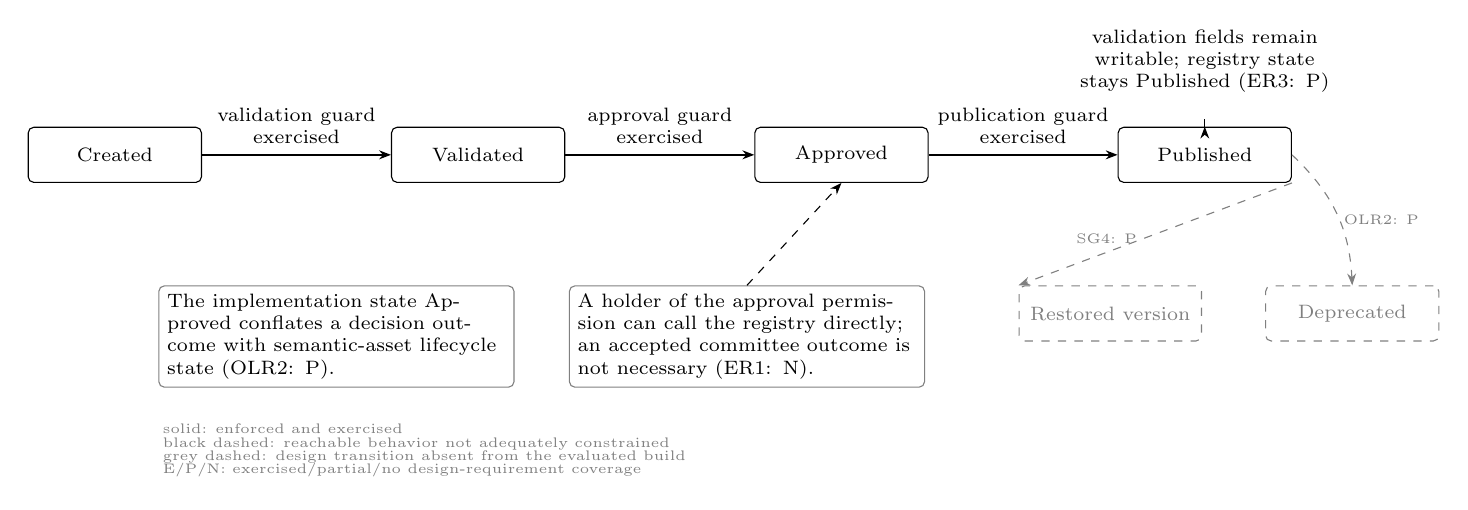
\begin{tikzpicture}[
  st/.style={draw, rounded corners=2pt, minimum height=7mm,
             minimum width=22mm, inner xsep=4pt, align=center, font=\scriptsize},
  absent/.style={st, draw=gray, dashed, text=gray},
  note/.style={draw=gray, rounded corners=2pt, align=left, text width=43mm,
              inner sep=3pt, font=\scriptsize},
  ed/.style={-{Stealth[length=1.5mm]}, thick},
  unenf/.style={-{Stealth[length=1.5mm]}, dashed},
  gone/.style={-{Stealth[length=1.5mm]}, dashed, draw=gray, text=gray},
  lbl/.style={font=\scriptsize, align=center, fill=white, inner sep=0.8pt},
  glbl/.style={font=\tiny, inner sep=1.5pt, text=gray},
]
\node[st] (c) {Created};
\node[st, right=24mm of c] (v) {Validated};
\node[st, right=24mm of v] (a) {Approved};
\node[st, right=24mm of a] (p) {Published};

\draw[ed] (c) -- node[lbl, midway, above=1mm]{validation guard\\exercised} (v);
\draw[ed] (v) -- node[lbl, midway, above=1mm]{approval guard\\exercised} (a);
\draw[ed] (a) -- node[lbl, midway, above=1mm]{publication guard\\exercised} (p);

\draw[unenf] (p.north) to[out=65,in=115,looseness=5]
  node[lbl, above, yshift=4mm, text width=38mm]
  {validation fields remain writable; registry state stays Published (ER3: P)} (p.north);

\node[note, below=13mm of a, xshift=-12mm] (u)
  {A holder of the approval permission can call the registry directly; an accepted committee outcome is not necessary (ER1: N).};
\draw[unenf] (u.north) -- (a.south);

\node[note, below=13mm of v, xshift=-18mm] (s)
  {The implementation state Approved conflates a decision outcome with semantic-asset lifecycle state (OLR2: P).};

\node[absent, below=13mm of p, xshift=-12mm] (r) {Restored version};
\node[absent, right=8mm of r] (d) {Deprecated};
\draw[gone] (p.south east) -- node[glbl, left, pos=0.55]{SG4: P} (r.north west);
\draw[gone] (p.east) to[bend left=22]
  node[glbl, right, pos=0.55]{OLR2: P} (d.north);

\node[glbl, below=4mm of s.south west, anchor=north west, align=left]
  {solid: enforced and exercised\\[-0.4mm]
   black dashed: reachable behavior not adequately constrained\\[-0.4mm]
   grey dashed: design transition absent from the evaluated build\\[-0.4mm]
   E/P/N: exercised/partial/no design-requirement coverage};
\end{tikzpicture}%
}
\caption{Implemented lifecycle-state guards and material gaps relative to the
current design requirements. The self-loop denotes a writable validation
record while the registry state remains \emph{Published}; it is not a backward
lifecycle transition.}
\label{fig:enforcement}
\end{figure*}

Figure~\ref{fig:enforcement} summarizes which lifecycle transitions are
enforced in the evaluated build and relates the principal defects to the
current design requirements. It also separates three facts that the earlier
figure could blur: \emph{Approved} is an implementation-specific registry
state rather than the design model's decision status; rewriting validation
fields does not move a published asset back to \emph{Validated}; and direct
approval by a permission holder leaves the collective outcome unnecessary.

Table~\ref{tab:coverage} records seventeen legacy implementation requirements as exercised and
five as specified without a corresponding implementation. The design-level
crosswalk gives a different and more relevant result: of the 36 requirements
derived in Sections~\ref{sec:governance_requirements}--\ref{sec:safeguards},
two have direct exercised support, sixteen have partial support, and eighteen
have no corresponding implementation. The difference is expected because the
design requirements specify cross-layer bindings and institutional safeguards
that the earlier implementation suite was not constructed to test. The suite
comprises 180 tests across eight files, with no focused or skipped tests; all
pass in the clean reproduction at the cited revision. Over the explicitly
declared contract boundary, instrumented coverage is 80.12\% (137/171)
statements, 64.89\% (122/188) branches, 73.61\% (53/72) functions, and
79.49\% (186/234) lines. These measurements expose residual unexecuted code
and support EQ3, but neither test quantity nor coverage percentage is treated
as a quality or conformance score.

Authorization enforceability is exercised primarily through negative
paths that cover unauthorized callers, invalid lifecycle orderings, temporal
and objection constraints, invalid arguments, and attempted bypasses. The
corresponding positive paths prevent a rejected call alone from being mistaken
for evidence that the intended caller can complete the operation. A permission
bit is a numbered Boolean flag that enables a particular action. The tests,
for example, establish that granting bit 28 to a role confers proposal rights
on every holder of that role, while revoking bit 29 withdraws objection rights
from that role and leaves them intact for a role that retains the bit.

Accountability and lifecycle traceability rest on the events emitted by
the lifecycle registry. Each governed transition records the address of
the acting party, and where a transition is executed by a governance
contract the recorded address is that contract rather than the account
that submitted the transaction. The stored record of a semantic asset
preserves its submitter, submission time, content hash and version, and
successive versions of one dataset remain individually addressable, so
the sequence of transitions applied to a dataset can be reconstructed
from on-chain state.

What this establishes is attribution of technical execution: a
transition can be traced to the governance mechanism that carried it
out. Two further links are required for the institutional
accountability described in Section~\ref{sec:accountability}, and they
are of different kinds. The binding between an account and a legal
person belongs to an identity layer that this architecture treats as
external: the artifact records addresses and stores an attestation at
onboarding, but verifying that attestation is the responsibility of the
credential infrastructure rather than of the governance contracts. The
binding between a transition and the deliberation behind it is, by
contrast, within scope and incomplete: the individual votes are recorded
by the governance contracts as their own events, but the registry record
carries no reference to the proposal that authorized the transition, so
the two event streams cannot be related without off-chain correlation.

Two limits on the ordering guarantee should be stated precisely. The
registry enforces two forward edges---a graph cannot be approved before it
has passed validation, and cannot be published before it has been
approved---together with idempotence on approval and on publication.
Backward transitions are not constrained: the validation result of an
approved or published graph remains writable, and no mechanism withdraws or
supersedes a published state. The order in which the two governance bodies
act is likewise not enforced by the registry.

The evaluation also identifies conditions under which the implemented
safeguards do not hold, each demonstrated by an executed test rather than
inferred from the contract text. Approval and publication gate on the
syntactic validation result alone, so a graph that failed semantic
validation can reach publication. A single role holds the permissions to
submit, validate and approve, so separation of duties is not enforced
on-chain. The published asset identifier is stored without any verified
correspondence to the content hash, and the same identifier can be attached
to more than one graph. Publishing a new version leaves its predecessor
published. The attestation recorded at onboarding expires but is not
consulted when a document is submitted. The consortium quorum is configured
at zero, so a single vote carries a proposal to a successful state. These
findings bound the claims made above and indicate where the evaluated build
requires revision or completion rather than further contract-level evaluation.

\subsection{Supplemental Local Decision-to-Publication Episode}
\label{sec:publication_episode}

The baseline identifies a central RQ2 gap: a collective decision can cause a
registry change but is not necessary for it, and no receipt verifies the
corresponding off-chain publication. To test a concrete repair, a separate
artificial integration episode implements one single-call publication profile
in \texttt{BoundPublication.sol}, using the existing
\texttt{ValidationCommittee} and voting token. This episode does not replace
the baseline implementation, upgrade its 36 requirement classifications, or
attribute new code to the earlier evaluated revision. The source, synthetic
RDF fixture, adapter, tests, results, and review forms are under
\texttt{reproducibility/paper-b/publication/} in the supplemental revision.\footnote{Supplemental reviewer entry point:
\url{https://github.com/alexbafana/MKM-POL21-2025/tree/codex/paper-b-reproducibility/reproducibility/paper-b/publication}. The development URL must be replaced by the fixed evaluated commit before submission.}

The unit of analysis is one exact publication authorization for an immutable
dataset/version record. Its content digest is Keccak-256 over UTF-8 N-Quads
canonicalized using RDFC-1.0 through the lockfile-pinned
\texttt{rdf-canonize} version 5.0.0. The synthetic employment fixture is not an
extraction dataset or a prediction about WoodHive. A narrow executable rule
requires parseable N-Quads, one permitted employment classification literal,
and a source IRI. This supplies a transparent test prerequisite rather than
an estimate of NLP, EMTAK, or general semantic-validation accuracy.

The executed chain has five steps. First, a producer submits a stable
chain/contract/dataset/version identifier, content digest, and model digest;
the version cannot be overwritten. Second, a distinct validator submits both
syntax and semantic outcomes plus a validation-evidence digest. Both outcomes
must pass, and validation cannot be rewritten after the version has progressed.
Third, the committee votes on the exact authorization call. Three local voters
have equal weight and a 34\% quorum; two votes succeed while one is insufficient.
The authorization fixes the asset, expiry, and exact proposal identifier.
The receiving contract checks that the derived single-call proposal is in the
Governor's Executed state during its callback. A direct permission holder
cannot authorize, and an accepted relay-wrapped call cannot substitute for that
exact proposal.

Fourth, the appointed adapter checks the authorization, expiry, and submitted
content before writing a content-addressed object to a local filesystem RDF
store. It then reads back and canonicalizes the object and compares its digest
with the approved digest. Fifth, the adapter submits the proposal identifier,
observed digest, publication identifier, and receipt digest. The registry
confirms only the authorized version and matching content, records the receipt,
and emits the version, decision, publication identifier, receipt digest, and
adapter address. The saved JSON manifest also identifies the chain, registry,
model/evidence digests, and confirmation transaction. An offline verifier
recomputes the object and receipt digests; the execution test independently
asserts the corresponding registry state and event arguments. Offline
verification is an integrity check, not an independent replay of blockchain
history.

\begin{table*}[t]
\centering\footnotesize
\caption{Supplemental publication episode: executed evidence and residual boundaries}
\label{tab:publication_episode}
\begin{tabular}{@{}p{4.0cm}p{7.0cm}p{6.0cm}@{}}
\toprule
\textbf{Property} & \textbf{Executed check} & \textbf{Inferential boundary} \\
\midrule
Decision binding (CR1, ER1) & Exact committee proposal is recorded; direct approval, insufficient quorum, and relay-wrapped substitution fail. & One fixed single-call publication profile; no compound plan. \\
Validation prerequisite (CR4, ER3) & Syntax and semantic flags both required; self-validation and later evidence rewriting fail. & Narrow fixture rule; validator remains trusted. \\
Content correspondence (ER4--ER5) & Canonical RDF is written/read locally; changed input and corrupted read-back are rejected; equivalent blank-node fixtures have equal digests. & Local store only; not a canonicalization conformance suite or live DKG. \\
Attributable confirmation (ER5--ER6, SG2) & Decision/version/digest/adapter/receipt links asserted; wrong decision, identifier, adapter, or empty receipt rejected. & Adapter is trusted to report read-back truth; failure receipts remain incomplete. \\
Expiry and replay (ER3, ER6) & Expired authorization and repeated confirmation/execution rejected. & No expiry recovery or missing-receipt escalation. \\
\bottomrule
\end{tabular}
\end{table*}

The supplemental suite executed 22 tests successfully. These comprise the
complete positive path and negative or equivalence checks for direct approval,
relay substitution, quorum failure, publication without authorization, syntax
or semantic failure, producer self-validation, duplicate versions, evidence
rewriting, changed content, corrupted read-back, wrong decision or identifier,
unappointed adapter, absent receipt, replay, expiry, canonicalization
invariance, and invalid or unsupported fixture data. The full test names,
execution log, local object, receipt manifest, and integrity-check output are
supplied. These tests are additional to the baseline's 180 tests in eight files;
the baseline coverage percentages do not measure the new contract.

This episode strengthens the feasibility evidence for the single-publication
clauses of CR1, CR4, and ER1--ER6 and the receipt-lineage aspect of SG2. It does
not establish complete satisfaction of those requirements. The on-chain
confirmation transaction is atomic and replay-protected, but filesystem
publication and chain confirmation are not one atomic transaction: a write
followed by failed confirmation can leave an unconfirmed object. The validator
and adapter are fixed trusted principals; a dishonest attestation is not
cryptographically excluded. Distinct addresses demonstrate technical role
separation, not independent institutions. The inherited permission manager
retains its administrative and participation limitations. Compound plans,
restoration, deprecation, legal policies, emergency review, censorship,
missing-receipt escalation, and long-term storage availability remain untested.

Independent design review is prepared but not reported as completed. A
prefilled 36-row review sheet pairs each full requirement with the original
status, evidence, and unmet clauses. A five-question walkthrough asks an
independent assessor to challenge exact decision/version binding, separation
of validation and authorization, receipt linkage, trust assumptions, and unmet
clauses. A second operator can reproduce both episodes using the supplied
commands and return environment records and discrepancies. These materials
reduce review preparation without turning automated checks into independent
expert findings; no inter-rater agreement or institutional endorsement is
claimed.

\subsection{Reproducibility and Artifact Availability}
\label{sec:artifact_availability}

The public artifact is organized for reviewer-first navigation rather than as
an undifferentiated development snapshot. The repository root links directly
to \texttt{reproducibility/paper-b/}, whose README states the claim boundary,
expected results, and fastest reproduction path. The package contains (i) an
artifact manifest with the evaluated contracts and pinned toolchain, (ii) a
36-row CSV crosswalk with evidence paths and limitations, (iii) the E/P/N
decision rules, (iv) an S1--S5 scenario index, (v) the executable reproduction
and manifest-validation scripts, (vi) reference results, (vii) a container
recipe, and (viii) a GitHub Actions workflow that uploads generated evidence.
Historical static-audit files are marked as such so that their earlier counts
are not confused with the present execution result.

Starting from a clean checkout of the cited commit, the complete
contract-level evaluation is invoked from the repository root by:
\begin{lstlisting}[language=bash,caption={One-command reproduction of the Section~6 evidence},label={lst:reproduce}]
bash reproducibility/paper-b/scripts/reproduce.sh
\end{lstlisting}
The script installs the lockfile-pinned dependencies, cleans generated
artifacts produced by Hardhat, the smart-contract build and test environment,
executes all tests, reruns from a clean build under
Solidity coverage, validates the manifest and crosswalk, and writes the
environment record, test log, coverage log, machine-readable coverage, and
manifest-check output to \texttt{results/generated/}. Node.js 22.14.0,
Corepack 0.31.0, Yarn 3.2.3, Hardhat 2.22.19, Solidity 0.8.20, and
\texttt{solidity-coverage} 0.8.16 define the reference CI/container
environment through the workflow, manifest, container recipe, package
metadata, and lockfile. A direct host run records its actual Node.js, Corepack,
Yarn, commit, and platform values in \texttt{environment.txt}; it must not be
described as a reference-environment run when those values differ. The
continuous-integration (CI) service executes the same command;
the workflow definition and run
history are public, and the run for the cited commit completed
successfully.\footnote{\url{https://github.com/alexbafana/MKM-POL21-2025/actions/runs/36997370222}}

Here, \emph{reproducible} means that the public command, at the cited commit
and in the declared or transparently recorded toolchain, regenerates the reported contract-test,
coverage, and crosswalk-check outputs. It does not mean that independent
researchers have already replicated the study, that other environments must
produce byte-identical logs, or that the system has demonstrated population
accuracy, semantic correctness, institutional workload scalability, or
production reliability. None of those properties is estimated by this
contract-level evaluation.

Some baseline test names and console messages call the local Created--Validated--Approved--Published
sequence an ``end-to-end workflow'' and display an OriginTrail DKG identifier.
Within this evaluation, that phrase denotes only the end of the contract
fixture: the identifier is a synthetic string stored by the registry, and no
OriginTrail service, RDF store, or publication adapter is contacted. The paper
therefore does not treat that test label as evidence of end-to-end knowledge
graph publication.

Table~\ref{tab:evidence_ledger} makes the numerical and scenario claims
auditable by pairing each reported outcome with its primary repository file
and the package-level check applied to it. Its purpose is not to repeat the
results, but to show reviewers where each count originates and which checks do
and do not validate it.

\begin{table*}[t]
\centering
\caption{Trace from reported evaluation outcomes to public repository evidence}
\label{tab:evidence_ledger}
\renewcommand{\arraystretch}{1.08}
\footnotesize
\setlength{\tabcolsep}{3pt}
\begin{tabular}{@{}p{4.0cm}p{7.0cm}p{6.2cm}@{}}
\toprule
\textbf{Reported outcome} & \textbf{Primary generated or source evidence} & \textbf{Independent check within the package} \\
\midrule
Eight test files; 180 passing tests & \texttt{results/generated/test-output.txt}; test sources under \texttt{packages/hardhat/test/} & \texttt{verify-manifest.mjs} counts test declarations, rejects focused/skipped tests, and compares the totals with \texttt{artifact-manifest.json}. \\
36 design requirements; 2 E, 16 P, 18 N & \texttt{requirements/coverage-crosswalk.csv}, including evidence path and limitation for every row & \texttt{verify-manifest.mjs} checks row count, identifier uniqueness, status totals, and existence of declared contract paths. \\
80.12\% statements, 64.89\% branches, 73.61\% functions, 79.49\% lines & \texttt{results/generated/coverage-output.txt}, \texttt{coverage.json}, and \texttt{lcov.info} & The reproduction script regenerates these files after a clean build; the manifest records the expected headline values. \\
Outcomes and boundaries of S1--S5 & \texttt{scenarios/S1-S5.md} and the referenced test sections & The crosswalk and test log expose whether each situation is exercised, partial, absent, or demonstrated as a gap. \\
Revision and environment & Git commit \texttt{3c55c690\ldots} and \texttt{results/generated/environment.txt} & The reproduction script records the checked-out commit and tool versions for each run. \\
\bottomrule
\end{tabular}
\end{table*}

The artifact contains no external empirical dataset. Its evaluation inputs
are deterministic local accounts, contract fixtures---repeatable test setups
that deploy the contracts and initialize their accounts and state---and the
requirement and scenario mappings included in the repository. These fixtures
are synthetic technical inputs, not observations of institutional behavior.
Generated logs are evidence of
a run, while the commit-pinned source, lockfile, scripts, and expected-result
manifest are the materials needed to repeat it. The full commit hash prevents
a moving branch from changing the cited evidence. The included
\texttt{CITATION.cff} and Zenodo metadata prepare archival deposit; no digital
object identifier (DOI) is
claimed until such a deposit exists.

All materials used to support the reported Section~\ref{sec:evaluation}
findings are public at the cited commit. There is no controlled or withheld
evidence on which a reported count or outcome depends. Files under
\texttt{results/generated/} are reproducible run outputs; the public reference
summary is a reviewer convenience rather than an additional evidence source;
historical audit files are contextual and do not determine the reported
counts. Only the planned archival release and DOI are provisional, and neither
is used as evidence.

Because the employment-extraction pipeline is outside the executed boundary,
the evaluation produces no per-item predictions, human reference labels,
label reconciliation or adjudication records, or threshold-sensitivity runs.
Consequently, there are no Run-0, Run-1, or Run-Var results to distinguish,
and no frozen prediction whose decision is changed by a threshold variation;
such materials are absent by design rather than withheld. EMTAK is used only
to explain the running-case classification context: no EMTAK mapping accuracy
is evaluated, and the artifact uses no \texttt{NOT\_EVALUATED} sentinel value.
Nor does the evaluation use a repository comparator for empirical outputs.
The script \texttt{verify-manifest.mjs} is instead an integrity checker: it
compares observed test-file, test, requirement, identifier, and status counts
with the public manifest and verifies that the contract paths declared in the
manifest exist. It
does not compare predictions with labels or estimate model performance.

\subsection{Discussion and Threats to Validity}
\label{sec:discussion}

The evaluation qualifies, rather than replaces, the design-stage answer to
each sub-research question. For RQ1, only OLR1 and OLR5 receive direct
exercised support; OLR2, OLR4, OLR6, and OLR9 are partially represented, and
the remaining six Organization-layer requirements have no corresponding
implementation. The role and permission registry implements
governance roles as sets of permission indices held at role scope, and
the evaluation establishes that rights are enforced per action, that
delegating a permission extends it to every holder of the role, and
that revocation withdraws it from the role as a whole. Selected
permissions governing the creation and update of semantic assets are
thus implemented and exercised. This is narrower than an answer to RQ1.
Whether the allocation of rights across the producer, validator,
authorizer and auditor roles is institutionally appropriate is not
established by test execution, and the evaluation in fact shows that it
is not: a single role holds the permissions to submit, validate and
approve, so separation of duties is not enforced on-chain. Deprecation,
named in RQ1, has no implementation at all, as no reachable function
withdraws or supersedes a published asset. The implementation therefore
supports selected enforcement mechanics but does not implement the
design-stage answer to RQ1 as a whole, especially its joint
asset/transition scope, governable administration, policy reference, and
distribution constraint.

For RQ2, none of CR1--CR6 and ER1--ER6 is fully covered: seven requirements
receive partial support and five have no corresponding implementation. The
artifact nevertheless implements two distinct decision procedures---an
optimistic procedure with an objection window in the consortium
contract, and a quorum-based vote in the validation committee---and
both are shown to execute lifecycle transitions on behalf of the
deciding body, with the transition attributed on-chain to that body
rather than to the submitting account. The binding of decisions to
transitions is nevertheless weaker than the design in
Section~\ref{sec:lifecycle_binding} describes. The lifecycle registry
authorizes approval by checking a permission bit; because the committee
holds that bit, a committee decision can drive the transition, but
nothing requires that it does. A collective decision is sufficient for
the transition and is not necessary to it. This is the principal
qualification on the answer to RQ2 and, by extension, on the main
research question: the artifact demonstrates that lifecycle transitions
\emph{can} be placed under decentralized authorization, not that the
present implementation forecloses unilateral action. The missing authorization
record, distinct execution states, canonicalization rule, and result receipt
also mean that the implemented path stops before the technical-confirmation
boundary specified by ER1--ER6.

For RQ3, SG1--SG4 and SG12 receive partial support, while SG5--SG11 have no
corresponding implementation. Technical event-level traceability is supported:
every governed
transition emits a durable record identifying the executing mechanism
and the affected asset, and the sequence of transitions applied to a
dataset is reconstructible from on-chain state. This is one of the
properties through which Section~\ref{sec:accountability} defines
accountability. Four stronger properties are not established. Attribution to
an institutional role requires an identity binding that the architecture
treats as external. Decision rationale and a bidirectional decision--asset
link require the registry to reference the authorizing proposal, which it
does not. Availability to external review depends on operating conditions
absent from a local execution environment. Persistence follows from the ledger rather than
from anything this evaluation demonstrates. Reversibility is not
supported: no mechanism restores a previous published state, and the
requirement is reported as specified but not implemented. Compliance is
addressed by design in Section~\ref{sec:compliance} but lies outside
what contract execution can establish; demonstrating it would require a
structured requirements walkthrough or review by legal experts, and is
left to future work. The implementation therefore supports fragments of
accountability, forward-only history, and failure termination, but it does not
implement the design-stage answer to RQ3. Legal adequacy and institutional
legitimacy would still require methods this evaluation does not apply even
after the missing representational and enforcement mechanisms were added.

\subsubsection{Relation of the Findings to Prior Work}

The evaluation first qualifies the lifecycle and provenance literature. Work
on knowledge graph ecosystems treats integration, continuous update,
publication, and provenance as connected lifecycle concerns, while provenance
models and traceability approaches make versions and derivations inspectable
\cite{Moreau2013PROV,Geisler2025KGLifecycle,Dibowski2024TraceabilityKG}. The
evaluated prototype supports part of that account: graph versions, content
hashes, model versions, transition events, and acting addresses remain
queryable. Its gaps show, however, that technical lineage is not yet
governance lineage. A registry event does not identify the proposal that
authorized it, and a stored publication identifier does not prove that the
approved graph was published. This result complements KG.gov's treatment of
knowledge graphs as a data-governance backbone and trustworthy-KG work on
human oversight and accountability
\cite{MeronoPenuela2025KGgov,Zhang2025TrustworthyKG}: representing data,
behavior, provenance, and oversight remains insufficient unless the
authorizing decision and resulting operation are linked bidirectionally.

Second, the results qualify general DAO-governance research. Proposal,
objection, voting, quorum, and temporal controls in the prototype correspond
to the mechanism families synthesized by Han et al. and to the configurable
governance architectures observed across operational DAOs
\cite{Han2025DAOReview,Riabokon2026ProgrammableGovernance}. Yet the zero
consortium quorum, direct approval path, and role capable of submission,
validation, and approval demonstrate why the presence of a voting contract
does not establish decentralized authority. This finding is consistent with
the 2026 live-governance study of 52 token protocols, which treats
concentration as a current control condition rather than inferring it from
launch allocation or holder counts \cite{Zukowski2026GovernanceConcentration}.
For institutional semantic assets, the analogous object of measurement is the
effective distribution of proposal, validation, authorization, execution, and
confirmation rights. OLR12 and SG10--SG11 extend that concern beyond token
holdings to independently accountable principals and incompatible duties, but
the evaluated build does not yet enforce or monitor those properties.

Third, the findings refine the model-driven DAO contribution. DAO-ML, ET-DM,
and DAOMod provide reusable organizational, coordination, execution,
token-economy, and voting-protocol constructs
\cite{Avanzo2024DAOML,Avanzo2025ETDM,Avanzo2025DAOMod,Avanzo2026DAOModCoordination}.
The present specialization adds a domain-specific chain from an immutable
semantic-asset version and evidence manifest through decision, scoped
authorization, exact operation, receipt, and resulting version. This chain
addresses the problem identified in the 2026 metagovernance review: when
governance spans deliberative forums, off-chain polling, nested organizations,
and cross-chain execution, decision points and responsibility can become
obscured \cite{Weidener2026Metagovernance}. The evaluation provides negative
support for the importance of that extension: without a scoped authorization,
canonical content binding, and attributable result receipt, a successful vote
and a later registry transition coexist without proving that the former
authorized the latter. The contribution is therefore not a claim that another
voting protocol solves knowledge graph governance, but a traceable
specialization that exposes where generic DAO mechanisms must be connected to
semantic-asset evidence and institutional mandates.

Across these comparisons, the evaluation both confirms and delimits the
paper's novelty claim. It confirms that lifecycle evidence, programmable
collective decisions, and institutional controls are complementary rather
than interchangeable. It delimits the claim because the prototype implements
only fragments of their required binding. The resulting open issues are not
merely additional contract features: they concern end-to-end evidence across
heterogeneous services, defensible and observable distributions of authority,
and the relation between programmable decisions and institutionally valid
mandates.

\subsubsection{Threats to Validity}

\emph{Construct validity} concerns whether the executed checks
represent the properties claimed. Test execution establishes that a
guard rejects an unauthorized caller and admits an authorized one; it
does not establish that the permission model expresses the
institutional allocation of authority correctly. Several assessment
criteria are operationalized narrowly by necessity: auditability is
measured as the emission of a record with identified fields, not as the
sufficiency of those fields for an institutional audit. The
demonstration that the objection window cannot be circumvented rests on
an argument over the reachable execution paths of the inherited
governance base contract, verified by inspection and exercised by test,
rather than on formal verification; introducing a timelock module would
change the executor and require that argument to be repeated. Explicit
E/P/N rules and clause-level limitations mitigate construct slippage, but the
single-author-team crosswalk remains susceptible to interpretation bias; an
independent coding study is therefore a suitable next validation step.

\emph{Internal validity} is limited by the form of the evidence.
The clean script, pinned lockfile, manifest checks, positive and negative
paths, and instrumented source coverage reduce the risk that results depend on
stale build products or an unreported subset of tests. They do not rule out
untested paths: branch coverage is 64.89\%, and the tests were developed with
the artifact. Configuration values are those of the test deployment and are
not defensible as institutional settings: the committee voting period is
thirty blocks, and the consortium quorum is zero, so a single vote carries a
proposal. These are parameters of the evaluated build rather than properties
of the design, and the reported observations hold only under them.

\emph{External validity} is bounded by the absence of deployment. The
artifact was executed in a single local environment with accounts
controlled by one party; no independent institution participated in a
governance decision, and no semantic asset was published to a
production decentralized knowledge graph. The running case is drawn
from a public-sector setting and was used to derive requirements, not
to instantiate the artifact operationally. Whether the mechanisms
remain workable when the deciding parties have divergent interests, or
when the volume of lifecycle transitions is institutional rather than
illustrative, is not addressed here.

\emph{Conclusion validity} concerns whether the reported observations
support the interpretations placed on them. The counts in
Section~\ref{sec:capability_assessment} are drawn from a single tree at
one immutable commit and are reproducible through
Listing~\ref{lst:reproduce}; the manifest checker independently verifies the
36 unique identifiers and the 2/16/18 status totals. Nevertheless, neither a
count of tests nor a coverage percentage is a measure of assurance: a
requirement covered by ten assertions is not thereby better satisfied than
one covered by three, and executed lines may implement an inadequate rule.
The statuses in Table~\ref{tab:coverage} should be read as a record of
what was exercised, while those in
Tables~\ref{tab:olr_coverage}--\ref{tab:sg_coverage} are an authorial
crosswalk from that evidence to the later platform-independent requirements;
neither is a graded assessment of quality. The
conditions reported at the end of
Section~\ref{sec:capability_assessment}, in which implemented
safeguards do not hold, are demonstrated by executed tests and are on
the same evidential footing as the positive results.

\paragraph{Answers to the evaluation questions.}
\emph{EQ1:} The complete design-to-implementation crosswalk classifies the 36
requirements as 2 E, 16 P, and 18 N; the prototype therefore directly
exercises only a small subset of the platform-independent design.
\emph{EQ2:} Within the implemented subset, positive and negative paths show
that selected permission, lifecycle-ordering, temporal, objection, and quorum
controls distinguish admitted operations from the tested violations. The same
execution evidence exposes bypasses and missing safeguards, including direct
approval, semantic-validation bypass, absent separation of duties, and
unverified publication identifiers.
\emph{EQ3:} A clean run executes 180 tests in eight files and yields 80.12\%
statement, 64.89\% branch, 73.61\% function, and 79.49\% line coverage over the
declared boundary; the tagged package and successful CI run reproduce these
results. This establishes reproducibility and measured structural breadth,
not conformance of unexecuted or institutionally defined properties.
\emph{EQ4:} The baseline does not support decision-to-publication binding.
The supplemental episode supports that chain for one local publication profile,
under trusted validator/adapter assumptions; neither episode establishes legal adequacy, institutional legitimacy, operation by independent
organizations, or production-scale suitability. Those claims remain outside
the evaluation boundary rather than being inferred from passing contract
tests.

Taken together, the evaluation establishes contract-level feasibility.
Selected authorization and transition mechanisms can be implemented as
smart contracts and exercised in the local configuration cited above,
transitions are attributable on-chain to the mechanism that executed
them, and temporal and quorum constraints hold against the execution
paths inspected and tested in that implementation---an argument over
reachable paths rather than formal verification, and one made under a
consortium quorum of zero. The supplemental episode adds a bounded local decision-to-publication chain,
but the evaluation does not establish general governance binding across all
on-chain and off-chain components, attribution to institutional roles, or operation by
independent organizations with divergent interests.

The distance between contract-level feasibility and institutional
deployment is occupied by the gaps reported in
Section~\ref{sec:capability_assessment}. The principal ones are binding
approval to the outcome of the collective decision rather than to a
permission bit, implementing the restoration and deprecation transitions
that the design specifies, and establishing configuration values that an
institution could defend. The evaluation identifies others: approval and
publication gate on the syntactic validation result alone, separation of
duties is not enforced across the submitting, validating and approving
roles, the published asset identifier is not bound to the approved
content hash, the attestation recorded at onboarding is not consulted
when a document is submitted, and a superseded version remains
published. These are matters of implementation rather than of further
measurement. Establishing institutional suitability is a separate empirical
and legal-evaluation problem requiring methods beyond source inspection and
test execution. Together with the related-work comparison, these limitations
define three open issues carried into Section~\ref{sec:conclusions}:
cross-system decision-to-result evidence, observable distribution of authority
among independent institutions, and the validity of the mandates and review
procedures that programmable governance operationalizes.




\section{Conclusions and Future Work}
\label{sec:conclusions}

This study addressed the gap between knowledge graph lifecycle engineering and model-driven DAO engineering through a design-science process. It used the institutional employment case and the literature knowledge base to derive 36 traceable requirements, specialized the Organization, Coordination, and Execution layers of DAOMod, added institutional safeguards, and mapped the resulting platform-independent design to an executable smart-contract prototype and reproducible tests. The WoodHive example connected each stage to a concrete consequence: whether a graph claiming that a company created 120 jobs may become, remain, or cease to be authoritative. The study thus produced and evaluated a governance design while keeping the evaluation claim bounded to the contract mechanisms and configuration actually exercised.

\paragraph{Answers to the Research Questions.}

\emph{Answer to RQ1.} DAO-ML requires domain adaptations that make the governed object and authority scope explicit. The specialization introduces identifiable and immutable semantic-asset versions, lifecycle states and compound transition plans, functional roles and committees, transition-scoped permissions, evidence requirements, and distribution constraints. In the running case, these constructs distinguish the curator who prepares a revised employment graph, the validator who checks it, the committee that authorizes publication, and the executor that performs it. This prevents a general permission over a data system from being mistaken for authority over every asset and every lifecycle operation.

\emph{Answer to RQ2.} ET-DM requires a traceable chain from proposal to observable semantic consequence. A proposal fixes the asset, transition plan, evidence manifest, initiator, and decision policy. An accepted outcome produces a scoped and expiring authorization rather than an unrestricted write permission. A binding then identifies the exact graph version, canonicalization and hashing methods, executor, and operation. Finally, an attributable receipt distinguishes successful confirmation from pending, failed, stale, or mismatched execution. For a replacement or restoration, the complete coupled plan must succeed atomically. These choices allow an auditor to distinguish a vote to publish the WoodHive graph from evidence that the approved graph was actually published.

\emph{Answer to RQ3.} Technically correct execution must be qualified by institutional safeguards. The proposed extensions bind technical identities to accountable mandates, preserve bidirectional lineage and decision rationale, implement correction and restoration as forward-only transitions, associate operations with jurisdiction-specific compliance profiles, constrain emergency authority and delegation, and address capture and liveness through prevention, detection, recovery, and residual-risk records. These safeguards do not make a blockchain decision lawful merely because it is recorded. They make the applicable authority, evidence, exceptional powers, and unresolved risks explicit enough to support institutional review.

\emph{Answer to the MRQ.} DAOMod can regulate an institutional knowledge graph lifecycle when its Organization, Coordination, and Execution layers are specialized around versioned semantic-asset transitions and connected by verifiable proposal, authorization, binding, receipt, and safeguard records. Decentralization must be treated as distributed accountable authority rather than as a count of blockchain addresses. This answer is conditional: the contract evaluation supports the feasibility of selected permission gates, voting and challenge mechanisms, version recording, temporal constraints, and event-level traceability, but not complete regulation of the lifecycle. The baseline build does not enforce decision-to-publication binding, separation of duties, semantic-validation gating, restoration, deprecation, content-to-publication hash correspondence, or institutionally defensible quorum settings. The supplemental profile exercises exact committee binding, distinct technical principals, a narrow validation gate, canonical content read-back and receipt confirmation for one local publication. This does not close the general institutional or lifecycle gaps.

\paragraph{Contribution and Significance.}
The paper does not claim novelty for knowledge graph lifecycles, provenance,
role-based access control, voting, smart contracts, or the base DAOMod
constructs individually. Its contribution is the design knowledge that
specializes and links them: semantic assets and versioned transitions in the
Organization layer; the proposal--decision--authorization--binding--receipt
chain across Coordination and Execution; an institutional safeguard overlay;
and an auditable requirements-to-implementation crosswalk. The theoretical
significance is the explicit separation of technical eligibility,
institutional authorization, and execution confirmation. The practical
significance is a design and evidence package that exposes both implemented
controls and missing links. Accordingly, the evaluation supports the
feasibility of selected mechanisms, not the novelty of their constituents or
the institutional suitability of the complete architecture.

\paragraph{Limitations, Open Issues, and Future Work.}
The limitations and open issues follow directly from the evaluation and its
comparison with prior work. The crosswalk was produced by the artifact's
authors, the tests use locally controlled accounts, branch coverage is
incomplete, and only a bounded local publication was exercised; live distributed
publication and legal and institutional adequacy remain unevaluated. Three open issues are therefore decisive: how to
preserve decision-to-result evidence across heterogeneous on-chain and
off-chain services; how to measure and enforce the live distribution of
authority across independently accountable institutions rather than infer
decentralization from roles, addresses, or token allocations; and how to bind
programmable decisions to jurisdiction-specific mandates, review, appeal, and
emergency procedures. Future work should first implement and test the complete
hybrid path with an RDF store, validation service, canonicalization procedure,
publication adapter, and attributable receipts. It should then subject the
requirements crosswalk and safeguard design to independent technical and legal
review, followed by multi-institutional evaluation with divergent participants
and realistic workloads. Comparative studies should vary committee
composition, quorum, concentration thresholds, delegation, and exceptional
procedures while monitoring liveness, capture, and selective non-execution.
Only this sequence can establish institutional suitability and transfer beyond
the Estonian employment case; additional passing contract tests alone cannot.

\section*{Declarations}

\noindent\textbf{Funding.}
This work was conducted in the context of the MKM-POL21 project,
``A Media-Driven Knowledge Graph Describing Estonia's Economic Development
and Its Governance Solutions,'' funded by the Estonian Ministry of Economic
Affairs and Communications.

\smallskip
\noindent\textbf{Competing interests.}
The authors declare that they have no competing interests.

\smallskip
\noindent\textbf{Data and code availability.}
The study uses no external empirical dataset. The contracts, test fixtures,
requirements crosswalk, scripts, and reference results supporting the
contract-level evaluation are publicly available at the immutable repository
revision cited in Section~\ref{sec:artifact_availability}:
\url{https://github.com/alexbafana/MKM-POL21-2025/tree/3c55c6903fe6fb38177889e22adf9639f8b9cda5/reproducibility/paper-b}.

\smallskip
\noindent\textbf{Use of generative artificial intelligence.}
During manuscript preparation, the authors used OpenAI ChatGPT and Codex to
assist with language editing and technical-consistency checks. The authors
reviewed and edited the resulting material and take full responsibility for
the content of the article.


% Can use something like this to put references on a page
% by themselves when using endfloat and the captionsoff option.
\ifCLASSOPTIONcaptionsoff
  \newpage
\fi



% trigger a \newpage just before the given reference
% number - used to balance the columns on the last page
% adjust value as needed - may need to be readjusted if
% the document is modified later
%\IEEEtriggeratref{8}
% The "triggered" command can be changed if desired:
%\IEEEtriggercmd{\enlargethispage{-5in}}

% references section

% can use a bibliography generated by BibTeX as a .bbl file
% BibTeX documentation can be easily obtained at:
% http://mirror.ctan.org/biblio/bibtex/contrib/doc/
% The IEEEtran BibTeX style support page is at:
% http://www.michaelshell.org/tex/ieeetran/bibtex/
%\bibliographystyle{IEEEtran}
% argument is your BibTeX string definitions and bibliography database(s)
%\bibliography{IEEEabrv,../bib/paper}
%
% <OR> manually copy in the resultant .bbl file
% set second argument of \begin to the number of references
% (used to reserve space for the reference number labels box)
\begin{thebibliography}{99}

\bibitem{Harris2013SPARQL}
S. Harris and A. Seaborne, eds.,
``SPARQL 1.1 Query Language,''
W3C Recommendation, Mar. 21, 2013. [Online]. Available:
\url{https://www.w3.org/TR/sparql11-query/}

\bibitem{serderidis2024d2kg}
K. Serderidis, I. Konstantinidis, G. Meditskos, V. Peristeras, and N. Bassiliades,
``d2kg: An integrated ontology for knowledge graph-based representation of government decisions and acts,''
\emph{Semantic Web}, vol. 15, pp. 1677--1699, 2024,
doi: 10.3233/SW-243535.

\bibitem{geisler2021transparency}
S. Geisler, M.-E. Vidal, C. Cappiello, B. F. L\'{o}scio, A. Gal, M. Jarke,
M. Lenzerini, P. Missier, B. Otto, E. Paja, B. Pernici, and J. Rehof,
``Knowledge-driven data ecosystems toward data transparency,''
\emph{J. Data Inf. Quality}, vol. 14, no. 1, Art. no. 3, pp. 1--12, 2022,
doi: 10.1145/3467022.

\bibitem{wood2021rtxkg2}
E. C. Wood \emph{et al.},
``RTX-KG2: A system for building a semantically standardized knowledge graph for translational biomedicine,''
\emph{BMC Bioinformatics}, vol. 23, Art. no. 400, 2022,
doi: 10.1186/s12859-022-04932-3.

\bibitem{seneviratne2025keepingkg}
O. Seneviratne,
``Keeping knowledge graphs alive: Constructing, growing, and sustaining knowledge graphs for the long haul,''
in \emph{Companion Proc. ACM Web Conf. 2025}, pp. 2549--2550, 2025.

\bibitem{papadopoulou2023argos}
E. Papadopoulou, A. Bardi, G. Kakaletris, D. Tziotzios, P. Manghi, and N. Manola,
``Data management plans as linked open data: Exploiting ARGOS FAIR and machine actionable outputs in the OpenAIRE research graph,''
\emph{J. Biomed. Semantics}, vol. 14, Art. no. 17, 2023,
doi: 10.1186/s13326-023-00297-5.

\bibitem{amaral2022prove}
G. Amaral, O. Rodrigues, and E. Simperl,
``ProVe: A pipeline for automated provenance verification of knowledge graphs against textual sources,''
\emph{Semantic Web}, vol. 15, no. 6, pp. 2159--2192, 2024,
doi: 10.3233/SW-233467.

\bibitem{Moreau2015Rationale}
L. Moreau, P. Groth, J. Cheney, T. Lebo, and S. Miles,
``The Rationale of PROV,''
\emph{Journal of Web Semantics},
vol. 35, pp. 235--257, 2015,
doi: 10.1016/j.websem.2015.04.001.

\bibitem{Sandhu1996RBAC}
R. S. Sandhu, E. J. Coyne, H. L. Feinstein, and C. E. Youman,
``Role-Based Access Control Models,''
\emph{IEEE Computer},
vol. 29, no. 2, pp. 38--47, 1996,
doi: 10.1109/2.485845.

%%%%%%%%%%%%%%%%%%%%%%%%%%%%%%%%

\bibitem{augustin2023understanding}
N. Augustin, A. Eckhardt, and A. W. de Jong,
``Understanding decentralized autonomous organizations from the inside,''
\emph{Electron. Markets}, vol. 33, Art. no. 38, 2023,
doi: 10.1007/s12525-023-00659-y.

\bibitem{rikken2023governance}
O. K. Rikken, M. F. W. H. A. Janssen, and Z. Roosenboom-Kwee,
``Governance impacts of blockchain-based decentralized autonomous organizations: An empirical analysis,''
\emph{Policy Design Pract.}, vol. 6, no. 4, pp. 465--487, 2023,
doi: 10.1080/25741292.2023.2270220.

\bibitem{Geisler2025KGLifecycle}
S. Geisler, C. Cappiello, I. Celino, D. Chaves-Fraga, A. Dimou, A. Iglesias-Molina, M. Lenzerini, A. Rula, D. Van Assche, S. Welten, and M.-E. Vidal,
``From Genesis to Maturity: Managing Knowledge Graph Ecosystems Through Life Cycles,''
\emph{Proceedings of the VLDB Endowment}, vol. 18, no. 5, pp. 1390--1397, 2025.
doi: 10.14778/3718057.3718067.

\bibitem{MeronoPenuela2025KGgov}
A. Mero{\~n}o-Pe{\~n}uela, E. Simperl, A. Kurteva, and I. Reklos,
``KG.gov: Knowledge Graphs as the Backbone of Data Governance in AI,''
\emph{Journal of Web Semantics}, vol. 85, Art. no. 100847, 2025.
doi: 10.1016/j.websem.2024.100847.

\bibitem{Zhang2025TrustworthyKG}
B. Zhang, E. Koutsiana, Y. Zhao, A. Mero{\~n}o-Pe{\~n}uela, and E. Simperl,
``Trustworthy Knowledge Graphs: Practices and Approaches,''
in \emph{Handbook on Neurosymbolic AI and Knowledge Graphs}, P. Hitzler, A. Dalal,
M. S. Mahdavinejad, and S. Saki Norouzi, Eds., Frontiers in Artificial Intelligence
and Applications, vol. 400. Amsterdam, The Netherlands: IOS Press, 2025,
pp. 363--384,
doi: 10.3233/FAIA250215.

\bibitem{Han2025DAOReview}
J. Han, J. Lee, and T. Li,
``A Review of DAO Governance: Recent Literature and Emerging Trends,''
\emph{Journal of Corporate Finance}, vol. 91, Art. no. 102734, 2025.
doi: 10.1016/j.jcorpfin.2025.102734.

\bibitem{Weidener2026Metagovernance}
L. Weidener, L. Bishop-Currey, and K. Compton,
``The Metagovernance Trilemma Across Decentralized Autonomous Organizations: A Scoping Review,''
\emph{Frontiers in Blockchain}, vol. 9, Art. no. 1759073, 2026.
doi: 10.3389/fbloc.2026.1759073.

\bibitem{Riabokon2026ProgrammableGovernance}
A. Riabokon,
``Programmable Governance and Institutional Design in Decentralized Autonomous Organizations: A Comparative Study of RARI DAO, Arbitrum DAO, and Optimism DAO,''
\emph{Frontiers in Blockchain}, vol. 9, Art. no. 1890169, 2026.
doi: 10.3389/fbloc.2026.1890169.

\bibitem{Zukowski2026GovernanceConcentration}
Z. Zukowski,
``Auditing Governance Concentration Beyond Token Allocation: A Live-Governance Study of 52 Token Protocols,''
\emph{Frontiers in Blockchain}, vol. 9, Art. no. 1853465, 2026.
doi: 10.3389/fbloc.2026.1853465.

\bibitem{Avanzo2024DAOML}
S. Avanzo, A. Norta, J. Linares, C. Schifanella, and M. Hattingh,
``DAO-ML: A Modelling Language for the Specification of Decentralized Autonomous Organization Governance,''
in \emph{Proc. 6th Distributed Ledger Technology Workshop}, CEUR Workshop Proceedings, vol. 3791, 2024. [Online]. Available:
\url{https://ceur-ws.org/Vol-3791/paper3.pdf}

\bibitem{Avanzo2025ETDM}
S. Avanzo, A. Norta, J. Linares, C. Schifanella, and M. Hattingh,
``Extending Trusted DApp Modeling for Decentralized Autonomous Organization Development,''
in \emph{Blockchain and Applications, 6th International Congress}, Lecture Notes in Networks and Systems, vol. 1256, pp. 140--149, 2025.
doi: 10.1007/978-3-031-81928-5\_14.

\bibitem{Avanzo2025DAOMod}
S. Avanzo, D. Pautasso, I. Domenicale, A. Norta, J. Linares, C. Schifanella, M. Hattingh, and D. S. Mitwalli,
``DAOMod: A Modeling Method for Decentralized Autonomous Organization Development,''
\emph{Electronic Communications of the EASST}, vol. 84, pp. 1--22, 2025.
doi: 10.14279/eceasst.v84.2675.

\bibitem{Avanzo2025DAOMLtoSolidity}
S. Avanzo, M. Ottina, D. Pautasso, I. Domenicale, A. Norta, and C. Schifanella,
``DAO-ML to Solidity: A Scalable Code Generation Approach for Decentralized Autonomous Organization Development,''
in \emph{Proc. 2025 International Conference on Information Technology for Social Good}, pp. 353--361, 2025.
doi: 10.1145/3748699.3749812.

\bibitem{Avanzo2026DAOModCoordination}
S. Avanzo, D. Pautasso, I. Domenicale, A. Norta, C. Schifanella, and M. Hattingh,
``DAOMod: A Modeling Method for Token Economy and Voting Protocol Specification,''
in \emph{Society 5.0}, Communications in Computer and Information Science, vol. 2787, pp. 25--37, 2026.
doi: 10.1007/978-3-032-15463-7\_3.

\bibitem{Fensel2020KG}
D. Fensel \emph{et al.},
\emph{Knowledge Graphs: Methodology, Tools and Selected Use Cases}.
Cham, Switzerland: Springer, 2020,
doi: 10.1007/978-3-030-37439-6.

\bibitem{Cyganiak2014RDFConcepts}
R. Cyganiak, D. Wood, and M. Lanthaler, eds.,
``RDF 1.1 Concepts and Abstract Syntax,''
W3C Recommendation, Feb. 25, 2014. [Online]. Available:
\url{https://www.w3.org/TR/rdf11-concepts/}

\bibitem{Knublauch2017SHACL}
H. Knublauch and D. Kontokostas, eds.,
``Shapes Constraint Language (SHACL),''
W3C Recommendation, July 20, 2017. [Online]. Available:
\url{https://www.w3.org/TR/shacl/}

\bibitem{Atzori2017BlockchainGovernance}
M. Atzori,
``Blockchain Technology and Decentralized Governance: Is the State Still Necessary?''
\textit{Journal of Governance and Regulation},
vol. 6, no. 1, pp. 45--62, 2017,
doi: 10.22495/jgr\_v6\_i1\_p5.

%%%%%%%%%%%%%%%%%%%%%%%%%%%%%

\bibitem{Hogan2021KnowledgeGraphs}
A.~Hogan, E.~Blomqvist, M.~Cochez, C.~d'Amato, G.~de Melo,
C.~Gutierrez, J.~E.~Labra Gayo, S.~Kirrane, S.~Neumaier,
A.~Polleres, R.~Navigli, A.~Ngomo, S.~M.~Rashid,
A.~Rula, L.~Schmelzeisen, J.~F.~Sequeda, S.~Staab,
and A.~Zimmermann,
``Knowledge Graphs,''
\emph{ACM Computing Surveys},
vol.~54, no.~4, Art. no. 71, pp.~1--37, 2021,
doi: 10.1145/3447772.

\bibitem{Carroll2005NamedGraphs}
J.~J.~Carroll, C.~Bizer, P.~Hayes and P.~Stickler,
``Named Graphs, Provenance and Trust,''
in \emph{Proc. 14th Int. Conf. World Wide Web}, pp. 613--622, 2005,
doi: 10.1145/1060745.1060835.

\bibitem{Piscopo2017WikidataProvenance}
A.~Piscopo and L.-A.~Kaffee,
``Provenance Information in a Collaborative Knowledge Graph:
An Evaluation of Wikidata External References,''
in \emph{Proc. 16th Int. Semantic Web Conf. (ISWC)},
pp.~542--558, 2017,
doi: 10.1007/978-3-319-68288-4\_32.

\bibitem{Kassen2025BlockchainGovernance}
M.~Kassen,
``Blockchain and digital governance:
Decentralization of decision making policy,''
\emph{Review of Policy Research},
vol.~42, no.~1, pp.~95--121,
Jan.~2025.
doi: 10.1111/ropr.12585.
%\url{https://onlinelibrary.wiley.com/doi/10.1111/ropr.12585}

\bibitem{FaqirRhazoui2020DAOOverview}
Y.~El Faqir, J.~Arroyo, and S.~Hassan,
``An Overview of Decentralized Autonomous Organizations
on the Blockchain,''
In \emph{Proceedings of the 16th International Symposium
on Open Collaboration}, ACM, 2020.
doi: 10.1145/3412569.3412579.

\bibitem{Tanvir2021EstBERT}
H. Tanvir, C. Kittask, S. Eiche, and K. Sirts,
``EstBERT: A Pretrained Language-Specific BERT for Estonian,''
in \emph{Proceedings of the 23rd Nordic Conference on Computational Linguistics (NoDaLiDa)},
Reykjavik, Iceland, 2021, pp. 11--19. [Online]. Available:
\url{https://aclanthology.org/2021.nodalida-main.2/}

\bibitem{Grootendorst2020KeyBERT}
M.~Grootendorst,
``KeyBERT: Minimal Keyword Extraction with BERT,''
Zenodo, ver. 0.3.0, 2020,
doi: 10.5281/zenodo.4461265.

\bibitem{Dibowski2024TraceabilityKG}
H.~Dibowski,
``Full Traceability and Provenance for Knowledge Graphs,''
in \emph{Proceedings of the 14th International Conference on
Formal Ontology in Information Systems (FOIS 2024)},
Frontiers in Artificial Intelligence and Applications,
vol.~394, pp.~223--237,
IOS Press, 2024.
doi: 10.3233/FAIA241309.

\bibitem{Lebo2013PROVO}
T.~Lebo, S.~Sahoo and D.~McGuinness,
``PROV-O: The PROV Ontology,''
W3C Recommendation, Apr. 30, 2013. [Online]. Available:
\url{https://www.w3.org/TR/prov-o/}

\bibitem{Schwabe2020KGTrustGovernance}
D.~Schwabe, C.~Laufer, and P.~Casanovas,
``Knowledge Graphs: Trust, Privacy, and Transparency
from a Legal Governance Approach,''
\emph{Law in Context: A Socio-legal Journal},
vol.~37, no.~1, pp. 24--41, 2020,
doi: 10.26826/law-in-context.v37i1.126.

\bibitem{Moreau2013PROV}
L.~Moreau and P.~Missier, eds.,
``PROV-DM: The PROV Data Model,''
W3C Recommendation, Apr. 30, 2013. [Online]. Available:
\url{https://www.w3.org/TR/prov-dm/}

\bibitem{Hassan2021DAO}
S.~Hassan and P.~De Filippi,
``Decentralized Autonomous Organization,''
\emph{Internet Policy Review},
vol.~10, no.~2, Art. no. 1556, 2021,
doi: 10.14763/2021.2.1556.

\bibitem{hevner2004design}
A. R. Hevner, S. T. March, J. Park, and S. Ram,
``Design science in information systems research,''
\textit{MIS Quarterly}, vol.~28, no.~1, pp.~75--105, 2004, doi: 10.2307/25148625.

\end{thebibliography}

% that's all folks
\end{document}
